% Options for packages loaded elsewhere
\PassOptionsToPackage{unicode}{hyperref}
\PassOptionsToPackage{hyphens}{url}
\PassOptionsToPackage{dvipsnames,svgnames*,x11names*}{xcolor}
%
\documentclass[
]{report}
\usepackage{lmodern}
\usepackage{amsmath}
\usepackage{ifxetex,ifluatex}
\ifnum 0\ifxetex 1\fi\ifluatex 1\fi=0 % if pdftex
  \usepackage[T1]{fontenc}
  \usepackage[utf8]{inputenc}
  \usepackage{textcomp} % provide euro and other symbols
  \usepackage{amssymb}
\else % if luatex or xetex
  \usepackage{unicode-math}
  \defaultfontfeatures{Scale=MatchLowercase}
  \defaultfontfeatures[\rmfamily]{Ligatures=TeX,Scale=1}
\fi
% Use upquote if available, for straight quotes in verbatim environments
\IfFileExists{upquote.sty}{\usepackage{upquote}}{}
\IfFileExists{microtype.sty}{% use microtype if available
  \usepackage[]{microtype}
  \UseMicrotypeSet[protrusion]{basicmath} % disable protrusion for tt fonts
}{}
\makeatletter
\@ifundefined{KOMAClassName}{% if non-KOMA class
  \IfFileExists{parskip.sty}{%
    \usepackage{parskip}
  }{% else
    \setlength{\parindent}{0pt}
    \setlength{\parskip}{6pt plus 2pt minus 1pt}}
}{% if KOMA class
  \KOMAoptions{parskip=half}}
\makeatother
\usepackage{xcolor}
\IfFileExists{xurl.sty}{\usepackage{xurl}}{} % add URL line breaks if available
\IfFileExists{bookmark.sty}{\usepackage{bookmark}}{\usepackage{hyperref}}
\hypersetup{
  pdftitle={Ovarian Cancer Histotypes: Report of Statistical Findings},
  pdfauthor={Derek Chiu},
  colorlinks=true,
  linkcolor=Maroon,
  filecolor=Maroon,
  citecolor=Blue,
  urlcolor=Blue,
  pdfcreator={LaTeX via pandoc}}
\urlstyle{same} % disable monospaced font for URLs
\usepackage[margin=1in]{geometry}
\usepackage{longtable,booktabs}
\usepackage{calc} % for calculating minipage widths
% Correct order of tables after \paragraph or \subparagraph
\usepackage{etoolbox}
\makeatletter
\patchcmd\longtable{\par}{\if@noskipsec\mbox{}\fi\par}{}{}
\makeatother
% Allow footnotes in longtable head/foot
\IfFileExists{footnotehyper.sty}{\usepackage{footnotehyper}}{\usepackage{footnote}}
\makesavenoteenv{longtable}
\usepackage{graphicx}
\makeatletter
\def\maxwidth{\ifdim\Gin@nat@width>\linewidth\linewidth\else\Gin@nat@width\fi}
\def\maxheight{\ifdim\Gin@nat@height>\textheight\textheight\else\Gin@nat@height\fi}
\makeatother
% Scale images if necessary, so that they will not overflow the page
% margins by default, and it is still possible to overwrite the defaults
% using explicit options in \includegraphics[width, height, ...]{}
\setkeys{Gin}{width=\maxwidth,height=\maxheight,keepaspectratio}
% Set default figure placement to htbp
\makeatletter
\def\fps@figure{htbp}
\makeatother
\setlength{\emergencystretch}{3em} % prevent overfull lines
\providecommand{\tightlist}{%
  \setlength{\itemsep}{0pt}\setlength{\parskip}{0pt}}
\setcounter{secnumdepth}{5}
\usepackage{titlesec, blindtext, color, float}

\titleformat{\chapter}[display]
  {\Huge\bfseries}
  {}
  {0pt}
  {\thechapter.\ }

\titleformat{name=\chapter,numberless}[display]
  {\Huge\bfseries}
  {}
  {0pt}
  {}

\titlespacing*{\chapter}{0pt}{0pt}{40pt}

\renewcommand{\bibname}{References}
\usepackage{booktabs}
\usepackage{longtable}
\usepackage{array}
\usepackage{multirow}
\usepackage{wrapfig}
\usepackage{float}
\usepackage{colortbl}
\usepackage{pdflscape}
\usepackage{tabu}
\usepackage{threeparttable}
\usepackage{threeparttablex}
\usepackage[normalem]{ulem}
\usepackage{makecell}
\usepackage{xcolor}
\ifluatex
  \usepackage{selnolig}  % disable illegal ligatures
\fi
\usepackage[]{natbib}
\bibliographystyle{apalike}

\title{Ovarian Cancer Histotypes: Report of Statistical Findings}
\author{Derek Chiu}
\date{2021-02-22}

\begin{document}
\maketitle

{
\hypersetup{linkcolor=}
\setcounter{tocdepth}{1}
\tableofcontents
}
\listoftables
\listoffigures
\hypertarget{preface}{%
\chapter*{Preface}\label{preface}}
\addcontentsline{toc}{chapter}{Preface}

This report of statistical findings describes the classification of ovarian cancer histotypes using data from NanoString CodeSets.

Marina Pavanello conducted the initial exploratory data analysis, Cathy Tang implemented class imbalance techniques, Derek Chiu conducted the normalization and statistical analysis, and Lauren Tindale and Aline Talhouk are the project leads.

\hypertarget{introduction}{%
\chapter{Introduction}\label{introduction}}

Ovarian cancer has five major histotypes: high-grade serous carcinoma (HGSC), low-grade serous carcinoma (LGSC), endometrioid carcinoma (ENOC), mucinous carcinoma (MUC), and clear cell carcinoma (CCOC). A common problem with classifying these histotypes is that there is a class imbalance issue. HGSC dominates the distribution, commonly accounting for 70\% of cases in many patient cohorts, while the other four histotypes are spread over the rest of the cases.

In the NanoString CodeSets, we also run into a problem with trying to find suitable control pools to normalize the gene expression. For prospective NanoString runs, the pools can be specifically chosen, but for retrospective runs, we have to utilize a combination of common samples and common genes as references for normalization.

The supervised learning is performed under a consensus framework: we consider various classification algorithms and use evaluation metrics to help make decisions of which methods to carry forward for downstream analysis.

\hypertarget{methods}{%
\chapter{Methods}\label{methods}}

\hypertarget{data-processing}{%
\section{Data Processing}\label{data-processing}}

RNA was extracted from FFPE ovarian carcinoma samples and expression was quantified using NanoString nCounter. Samples were run in three CodeSets. Some samples or pools of samples were repeated across CodeSets for expression normalization. Normalizing CS2 to CS3 can easily follow the \href{https://dchiu911.shinyapps.io/PrOType/}{PrOType} method for HGSC subtypes because both CodeSets have pool samples. A different technique is implemented when normalizing across CS1, CS2, and CS3 where we use common samples and genes as reference sets.

\hypertarget{raw-data}{%
\subsection{Raw Data}\label{raw-data}}

NanoString CodeSets contained a mix of all probes of interest, six positive controls spiked-in at fixed proportional concentrations (0.125- 128 fM), and eight negative controls (probes without a corresponding target). Gene targets also included 5 housekeeping genes: POLR1B, SDHA, PGK1, ACTB, RPL19. Gene selection was made from top ranked differential gene expression analysis between ovarian cancer histotypes and molecular subtypes of HGSC, as well as containing some genes of interest from unrelated projects. Gene targets in each subsequent CodeSet were re-curated, where non-informative genes were dropped and new potential differentiating genes were added.

There are 3 NanoString CodeSets:

\begin{itemize}
\item
  CS1: OvCa2103\_C953

  \begin{itemize}
  \tightlist
  \item
    Samples = 412
  \item
    Genes = 275
  \end{itemize}
\item
  CS2: PrOTYPE2\_v2\_C1645

  \begin{itemize}
  \tightlist
  \item
    Samples = 1223
  \item
    Genes = 384
  \end{itemize}
\item
  CS3: OTTA2014\_C2822

  \begin{itemize}
  \tightlist
  \item
    Samples = 5424
  \item
    Genes = 532
  \end{itemize}
\end{itemize}

These datasets contain raw counts extracted straight from NanoString RCC files.

\hypertarget{housekeeping-genes}{%
\subsection{Housekeeping Genes}\label{housekeeping-genes}}

The first normalization step is to normalize all endogenous genes to housekeeping genes (POLR1B, SDHA, PGK1, ACTB, RPL19; reference genes expressed in all cells). We normalize by subtracting the average log\textsubscript{2} housekeeping gene expression from the log\textsubscript{2} endogenous gene expression:

log\textsubscript{2} endogenous expression - log\textsubscript{2} average housekeeping expression = relative expression

The updated CodeSet dimensions are now:

\begin{itemize}
\item
  CS1: OvCa2103\_C953

  \begin{itemize}
  \tightlist
  \item
    Samples = 412
  \item
    Genes = 256
  \end{itemize}
\item
  CS2: PrOTYPE2\_v2\_C1645

  \begin{itemize}
  \tightlist
  \item
    Samples = 1223
  \item
    Genes = 365
  \end{itemize}
\item
  CS3: OTTA2014\_C2822

  \begin{itemize}
  \tightlist
  \item
    Samples = 5424
  \item
    Genes = 513
  \end{itemize}
\end{itemize}

The number of genes are reduced by 19: 5 housekeeping, 8 negative, 6 positive (the latter 2 types are not used).

\hypertarget{common-samples-and-genes}{%
\subsection{Common Samples and Genes}\label{common-samples-and-genes}}

Since the reference pool samples only exist in CS2 and CS3, we need to find an alternative method to normalize all three CodeSets. One method is to select common samples and common genes that exist in all three. We found 72 common genes. Using the \texttt{summaryID} identifier, we also found 78 common summary IDs, translating to 320 samples. The number of samples that were matched to each CodeSet differed:

\begin{itemize}
\item
  CS1: OvCa2103\_C953

  \begin{itemize}
  \tightlist
  \item
    Samples = 93
  \item
    Genes = 72
  \end{itemize}
\item
  CS2: PrOTYPE2\_v2\_C1645

  \begin{itemize}
  \tightlist
  \item
    Samples = 87
  \item
    Genes = 72
  \end{itemize}
\item
  CS3: OTTA2014\_C2822

  \begin{itemize}
  \tightlist
  \item
    Samples = 140
  \item
    Genes = 72
  \end{itemize}
\end{itemize}

\hypertarget{overlap-of-common-samples-by-summary-id}{%
\subsubsection{Overlap of common samples by summary ID}\label{overlap-of-common-samples-by-summary-id}}

\begin{center}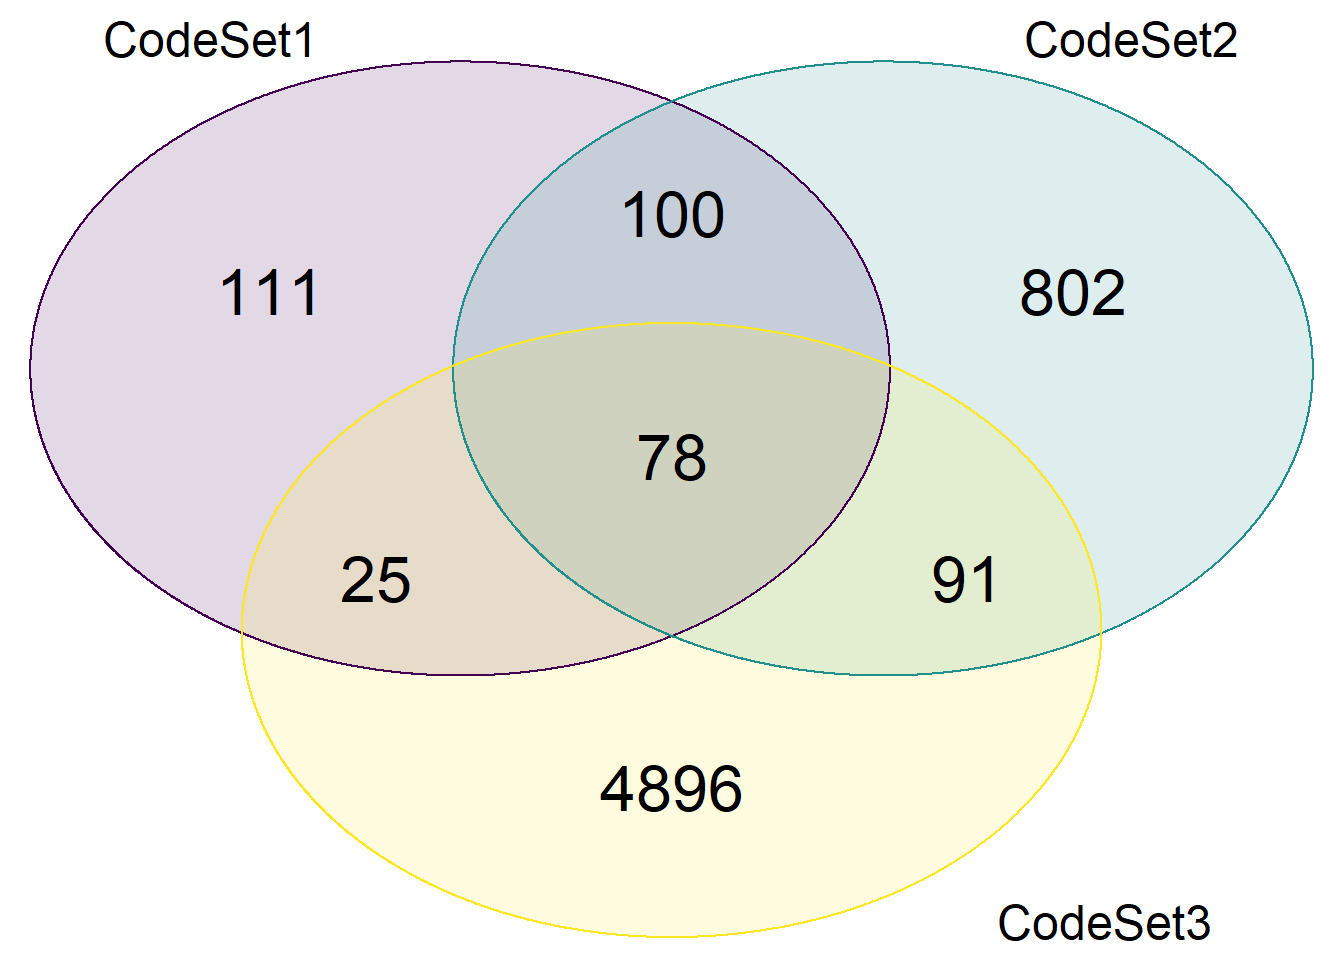
\includegraphics{OV_Histotypes_RSF_files/figure-latex/venn-id-1} \end{center}

\hypertarget{overlap-of-common-genes}{%
\subsubsection{Overlap of common genes}\label{overlap-of-common-genes}}

\begin{center}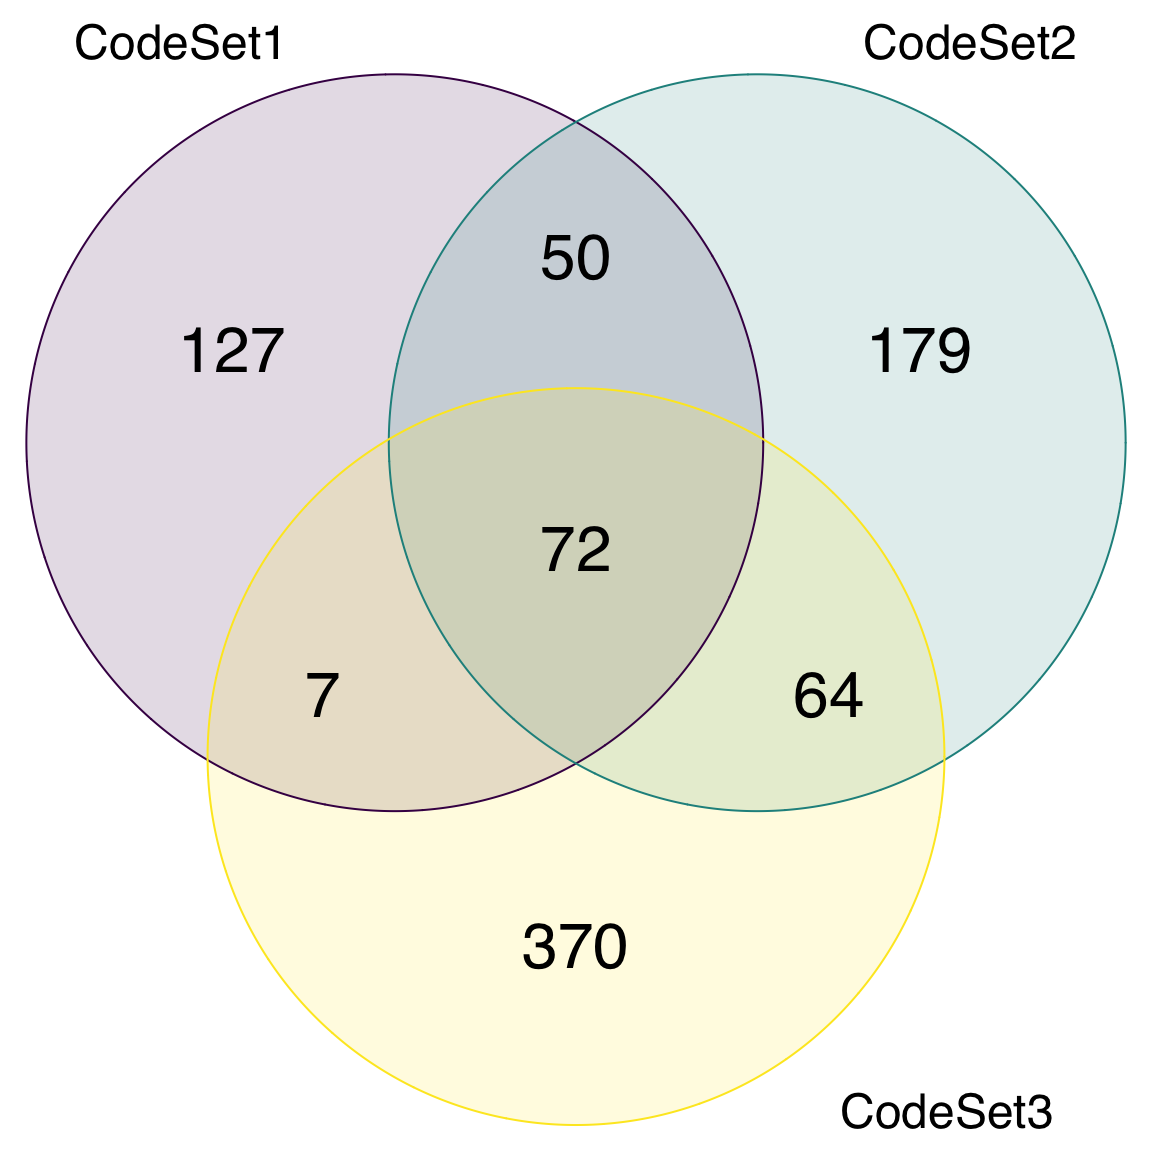
\includegraphics{OV_Histotypes_RSF_files/figure-latex/venn-genes-1} \end{center}

*Excluding housekeeping genes and controls

\hypertarget{cs1-training-set-generation}{%
\subsection{CS1 Training Set Generation}\label{cs1-training-set-generation}}

We use the reference method to normalize CS1 to CS3.

\begin{itemize}
\item
  CS1 reference set: duplicate samples from CS1

  \begin{itemize}
  \tightlist
  \item
    Samples = 25
  \item
    Genes = 72
  \end{itemize}
\item
  CS3 reference set: corresponding samples in CS3 also found in CS1 reference set

  \begin{itemize}
  \tightlist
  \item
    Samples = 20
  \item
    Genes = 72
  \end{itemize}
\item
  CS1 validation set: remaining CS1 samples with reference set removed

  \begin{itemize}
  \tightlist
  \item
    Samples = 387
  \item
    Genes = 72
  \end{itemize}
\end{itemize}

The final CS1 training set has 304 samples on 72 genes after normalization and keeping only the major histotypes of interest.

\hypertarget{cs2-training-set-generation}{%
\subsection{CS2 Training Set Generation}\label{cs2-training-set-generation}}

We use the pool method to normalize CS2 to CS3 so we can be consistent with the PrOType normalization when there are available pools.

\begin{itemize}
\item
  CS2 pools:

  \begin{itemize}
  \tightlist
  \item
    Samples = 12 (Pool 1 = 4, Pool 2 = 4, Pool 3 = 4)
  \item
    Genes = 365
  \end{itemize}
\item
  CS3 pools:

  \begin{itemize}
  \tightlist
  \item
    Samples = 22 (Pool 1 = 12, Pool 2 = 5, Pool 3 = 5)
  \item
    Genes = 513
  \end{itemize}
\item
  CS2 validation set: CS2 samples with pools removed

  \begin{itemize}
  \tightlist
  \item
    Samples = 1214
  \item
    Genes = 365
  \end{itemize}
\end{itemize}

The final CS2 training set has 945 samples on 136 (common) genes after normalization and keeping only the major histotypes of interest.

\hypertarget{cohort-distribution}{%
\subsection{Cohort Distribution}\label{cohort-distribution}}

CodeSets comprised samples from sites collected internationally as shown below. Note that the CS3 pools sample total (n=58) shown here include those that are not used as reference pools, following previous normalization methods. In particular, the distribution of CS3 pools actually used for normalization (n=22) is POOL1 = 12, POOL2 = 5, POOL3 = 5.

\begin{table}

\caption{\label{tab:cohort-dist}Cohort Distribution amongst CodeSets}
\centering
\begin{tabular}[t]{l|r|r|r}
\hline
cohort & cs1 & cs2 & cs3\\
\hline
MAYO & 6 & 63 & NA\\
\hline
MTL & 3 & 59 & NA\\
\hline
OOU & 108 & 43 & 19\\
\hline
OOUE & 32 & 30 & 11\\
\hline
VOA & 145 & 122 & 538\\
\hline
ICON7 & NA & 416 & NA\\
\hline
JAPAN & NA & 8 & NA\\
\hline
OVAR3 & NA & 150 & NA\\
\hline
POOL-CTRL & NA & 12 & NA\\
\hline
DOVE4 & NA & NA & 1160\\
\hline
POOL-1 & NA & NA & 31\\
\hline
POOL-2 & NA & NA & 14\\
\hline
POOL-3 & NA & NA & 13\\
\hline
TNCO & NA & NA & 691\\
\hline
\end{tabular}
\end{table}

\begin{table}

\caption{\label{tab:cohort-dist-distinct}Distinct Cohort Distribution amongst CodeSets}
\centering
\begin{tabular}[t]{l|r|r|r}
\hline
cohort & cs1 & cs2 & cs3\\
\hline
MAYO & 6 & 62 & NA\\
\hline
MTL & 3 & 59 & NA\\
\hline
OOU & 99 & 43 & 19\\
\hline
OOUE & 31 & 30 & 11\\
\hline
VOA & 136 & 107 & 452\\
\hline
ICON7 & NA & 383 & NA\\
\hline
JAPAN & NA & 8 & NA\\
\hline
OVAR3 & NA & 150 & NA\\
\hline
POOL-CTRL & NA & 3 & NA\\
\hline
DOVE4 & NA & NA & 1094\\
\hline
POOL-1 & NA & NA & 12\\
\hline
POOL-2 & NA & NA & 5\\
\hline
POOL-3 & NA & NA & 5\\
\hline
TNCO & NA & NA & 674\\
\hline
\end{tabular}
\end{table}

\hypertarget{normalization-between-codesets}{%
\section{Normalization Between CodeSets}\label{normalization-between-codesets}}

After normalization to housekeeping genes and filtering for the five major histotypes of interest, as determined by pathology review and/or IHC, two methods were used to normalize data between CodeSets.

\hypertarget{common-samples-method}{%
\subsection{Common Samples Method}\label{common-samples-method}}

The common samples method was used to normalize CodeSet1, 2, and 3, where common samples and genes were used as reference sets. Among the samples repeated in all CodeSets we normalized using either: a random set of 3 samples from each major histotype (random3; n=15), a random set of 2 samples from each major histotype (random2; n=10), or a random set of 1 sample from each major histotype (random1; n=5). In each case CodeSet3 expression (X\textsubscript{3}) was held fixed, while CodeSet1/2 expression (X\textsubscript{1} and X\textsubscript{2}) were normalized to CodeSet3 by subtracting the average gene expression from the CodeSet1/2 reference set (R\textsubscript{1} or R\textsubscript{2}) and adding the average gene expression of the CodeSet3 reference set (R\textsubscript{3}). Alternatively, X\textsubscript{1} (norm) = X\textsubscript{1} - R\textsubscript{1} + R\textsubscript{3} would calibrate CodeSet1 to CodeSet3.

\hypertarget{pools-method}{%
\subsection{Pools Method}\label{pools-method}}

The pools method was used to normalize CodeSet2 and CodeSet3. The three reference pools, regularly assayed mixes of samples representing all histotypes, were run in CodeSet2 and CodeSet3 only. CodeSet2 contained 12 reference pool samples (Pool 1 = 4, Pool 2 = 4, Pool 3 = 4) and CodeSet3 contained 22 reference pool samples (Pool 1 = 12, Pool 2 = 5, Pool 3 = 5). Similar to the common samples method, CodeSet2 was normalized to CodeSet3 via: X\textsubscript{2} (norm) = X\textsubscript{2} - R\textsubscript{2} + R\textsubscript{3} where R is the average expression of the reference pool samples in the respective CodeSet. This method of pool normalization was also used by PrOType to classify HGSC subtypes

\hypertarget{concordance-comparison}{%
\subsection{Concordance Comparison}\label{concordance-comparison}}

Concordance between CodeSets using the different normalization strategies was compared in common samples, excluding those used for the normalization, using Pearson's correlation coefficient (R\textsuperscript{2}), coefficient of accuracy (Ca), and Lin's concordance correlation (Rc = R\textsuperscript{2} x Ca).

\hypertarget{histotype-classification}{%
\section{Histotype Classification}\label{histotype-classification}}

We use 5 classification algorithms and 4 subsampling methods across 500 repetitions in the supervised learning framework for the Training Set, CS1 and CS2. The pipeline was run using SLURM batch jobs submitted to a partition on a CentOS 7 server. Implementations of the techniques below were called from the \href{https://alinetalhouk.github.io/splendid/}{splendid} package.

\begin{itemize}
\item
  Classifiers:

  \begin{itemize}
  \tightlist
  \item
    Random Forest
  \item
    SVM
  \item
    Adaboost
  \item
    Multinomial Regression Model with Ridge Penalty
  \item
    Multinomial Regression Model with LASSO Penalty
  \end{itemize}
\item
  Subsampling:

  \begin{itemize}
  \tightlist
  \item
    None
  \item
    Down-sampling
  \item
    Up-sampling
  \item
    SMOTE
  \end{itemize}
\end{itemize}

\hypertarget{validation}{%
\chapter{Validation}\label{validation}}

\hypertarget{full-data-distributions}{%
\section{Full Data Distributions}\label{full-data-distributions}}

The histotype distributions on the full data are shown below.

\begin{table}

\caption{\label{tab:dist-all-gr}All CodeSet Histotype Groups}
\centering
\begin{tabular}[t]{l|r|r|r}
\hline
hist\_gr & CS1 & CS2 & CS3\\
\hline
HGSC & 169 & 757 & 2453\\
\hline
non-HGSC & 196 & 373 & 677\\
\hline
\end{tabular}
\end{table}

\begin{table}

\caption{\label{tab:dist-all}All CodeSet Histotypes}
\centering
\begin{tabular}[t]{l|r|r|r}
\hline
revHist & CS1 & CS2 & CS3\\
\hline
CARCINOMA-NOS & 0 & 61 & 23\\
\hline
Carcinoma, NOS & 0 & 0 & 2\\
\hline
CCOC & 57 & 68 & 182\\
\hline
CCOC-MCT & 0 & 1 & 0\\
\hline
Cell-Line & 17 & 48 & 13\\
\hline
CTRL & 0 & 12 & 0\\
\hline
ENOC & 61 & 30 & 272\\
\hline
ENOC-CCOC & 0 & 7 & 0\\
\hline
ERROR & 0 & 3 & 0\\
\hline
HGSC & 169 & 757 & 2453\\
\hline
HGSC-MCT & 0 & 1 & 0\\
\hline
LGSC & 22 & 29 & 50\\
\hline
MBOT & 0 & 20 & 3\\
\hline
MET-NOP & 0 & 21 & 0\\
\hline
MIXED (ENOC/CCOC) & 0 & 0 & 1\\
\hline
MIXED (ENOC/LGSC) & 0 & 0 & 1\\
\hline
MIXED (HGSC/CCOC) & 0 & 0 & 1\\
\hline
mixed cell & 0 & 0 & 7\\
\hline
MMMT & 0 & 0 & 30\\
\hline
MUC & 20 & 61 & 77\\
\hline
Other (use when 6, 7, or 9 is not distinguished) or unknown if epithelial & 0 & 0 & 1\\
\hline
Other/Exclude & 0 & 0 & 8\\
\hline
SBOT & 19 & 10 & 3\\
\hline
Serous & 0 & 0 & 2\\
\hline
serous LMP & 0 & 0 & 1\\
\hline
SQAMOUS & 0 & 1 & 0\\
\hline
\end{tabular}
\end{table}

\begin{table}

\caption{\label{tab:dist-common}Common Summary ID CodeSet Histotypes}
\centering
\begin{tabular}[t]{l|r|r|r}
\hline
revHist & CS1 & CS2 & CS3\\
\hline
CCOC & 3 & 4 & 9\\
\hline
Cell-Line & 4 & 5 & 5\\
\hline
ENOC & 4 & 4 & 9\\
\hline
HGSC & 68 & 64 & 98\\
\hline
LGSC & 7 & 5 & 8\\
\hline
MUC & 7 & 5 & 11\\
\hline
\end{tabular}
\end{table}

\begin{table}

\caption{\label{tab:dist-major-hist}All CodeSet Major Histotypes}
\centering
\begin{tabular}[t]{l|r|r|r|r|r|r}
\hline
revHist & CS1 & CS2 & CS3 & CS1\_percent & CS2\_percent & CS3\_percent\\
\hline
CCOC & 57 & 68 & 182 & 17.3 & 7.2 & 6.0\\
\hline
ENOC & 61 & 30 & 272 & 18.5 & 3.2 & 9.0\\
\hline
HGSC & 169 & 757 & 2453 & 51.4 & 80.1 & 80.9\\
\hline
LGSC & 22 & 29 & 50 & 6.7 & 3.1 & 1.6\\
\hline
MUC & 20 & 61 & 77 & 6.1 & 6.5 & 2.5\\
\hline
\end{tabular}
\end{table}

\begin{table}

\caption{\label{tab:dist-cs1}CS1 Histotypes}
\centering
\begin{tabular}[t]{l|l|r}
\hline
CodeSet & revHist & n\\
\hline
CS1 & CCOC & 57\\
\hline
CS1 & Cell-Line & 17\\
\hline
CS1 & ENOC & 61\\
\hline
CS1 & HGSC & 169\\
\hline
CS1 & LGSC & 22\\
\hline
CS1 & MUC & 20\\
\hline
CS1 & SBOT & 19\\
\hline
\end{tabular}
\end{table}

\begin{table}

\caption{\label{tab:dist-cs2}CS2 Histotypes}
\centering
\begin{tabular}[t]{l|l|r}
\hline
CodeSet & revHist & n\\
\hline
CS2 & CARCINOMA-NOS & 61\\
\hline
CS2 & CCOC & 68\\
\hline
CS2 & CCOC-MCT & 1\\
\hline
CS2 & Cell-Line & 48\\
\hline
CS2 & CTRL & 12\\
\hline
CS2 & ENOC & 30\\
\hline
CS2 & ENOC-CCOC & 7\\
\hline
CS2 & ERROR & 3\\
\hline
CS2 & HGSC & 757\\
\hline
CS2 & HGSC-MCT & 1\\
\hline
CS2 & LGSC & 29\\
\hline
CS2 & MBOT & 20\\
\hline
CS2 & MET-NOP & 21\\
\hline
CS2 & MUC & 61\\
\hline
CS2 & SBOT & 10\\
\hline
CS2 & SQAMOUS & 1\\
\hline
\end{tabular}
\end{table}

\begin{table}

\caption{\label{tab:dist-cs3}CS3 Histotypes}
\centering
\begin{tabular}[t]{l|l|r}
\hline
CodeSet & revHist & n\\
\hline
CS3 & CARCINOMA-NOS & 23\\
\hline
CS3 & Carcinoma, NOS & 2\\
\hline
CS3 & CCOC & 182\\
\hline
CS3 & Cell-Line & 13\\
\hline
CS3 & ENOC & 272\\
\hline
CS3 & HGSC & 2453\\
\hline
CS3 & LGSC & 50\\
\hline
CS3 & MBOT & 3\\
\hline
CS3 & MIXED (ENOC/CCOC) & 1\\
\hline
CS3 & MIXED (ENOC/LGSC) & 1\\
\hline
CS3 & MIXED (HGSC/CCOC) & 1\\
\hline
CS3 & mixed cell & 7\\
\hline
CS3 & MMMT & 30\\
\hline
CS3 & MUC & 77\\
\hline
CS3 & Other (use when 6, 7, or 9 is not distinguished) or unknown if epithelial & 1\\
\hline
CS3 & Other/Exclude & 8\\
\hline
CS3 & SBOT & 3\\
\hline
CS3 & Serous & 2\\
\hline
CS3 & serous LMP & 1\\
\hline
\end{tabular}
\end{table}

\hypertarget{training-set-distributions}{%
\section{Training Set Distributions}\label{training-set-distributions}}

The training set distributions for CS1 and CS2 are shown below.

\begin{table}

\caption{\label{tab:training-dist-cs1}CS1 Training Set Histotypes}
\centering
\begin{tabular}[t]{l|r}
\hline
histotype & n\\
\hline
CCC & 57\\
\hline
ENOCa & 59\\
\hline
HGSC & 156\\
\hline
LGSC & 16\\
\hline
MUC & 16\\
\hline
\end{tabular}
\end{table}

\begin{table}

\caption{\label{tab:training-dist-cs2}CS2 Training Set Histotypes}
\centering
\begin{tabular}[t]{l|r}
\hline
histotype & n\\
\hline
CCOC & 68\\
\hline
ENOC & 30\\
\hline
HGSC & 757\\
\hline
LGSC & 29\\
\hline
MUC & 61\\
\hline
\end{tabular}
\end{table}

\hypertarget{normalization}{%
\section{Normalization}\label{normalization}}

\begin{center}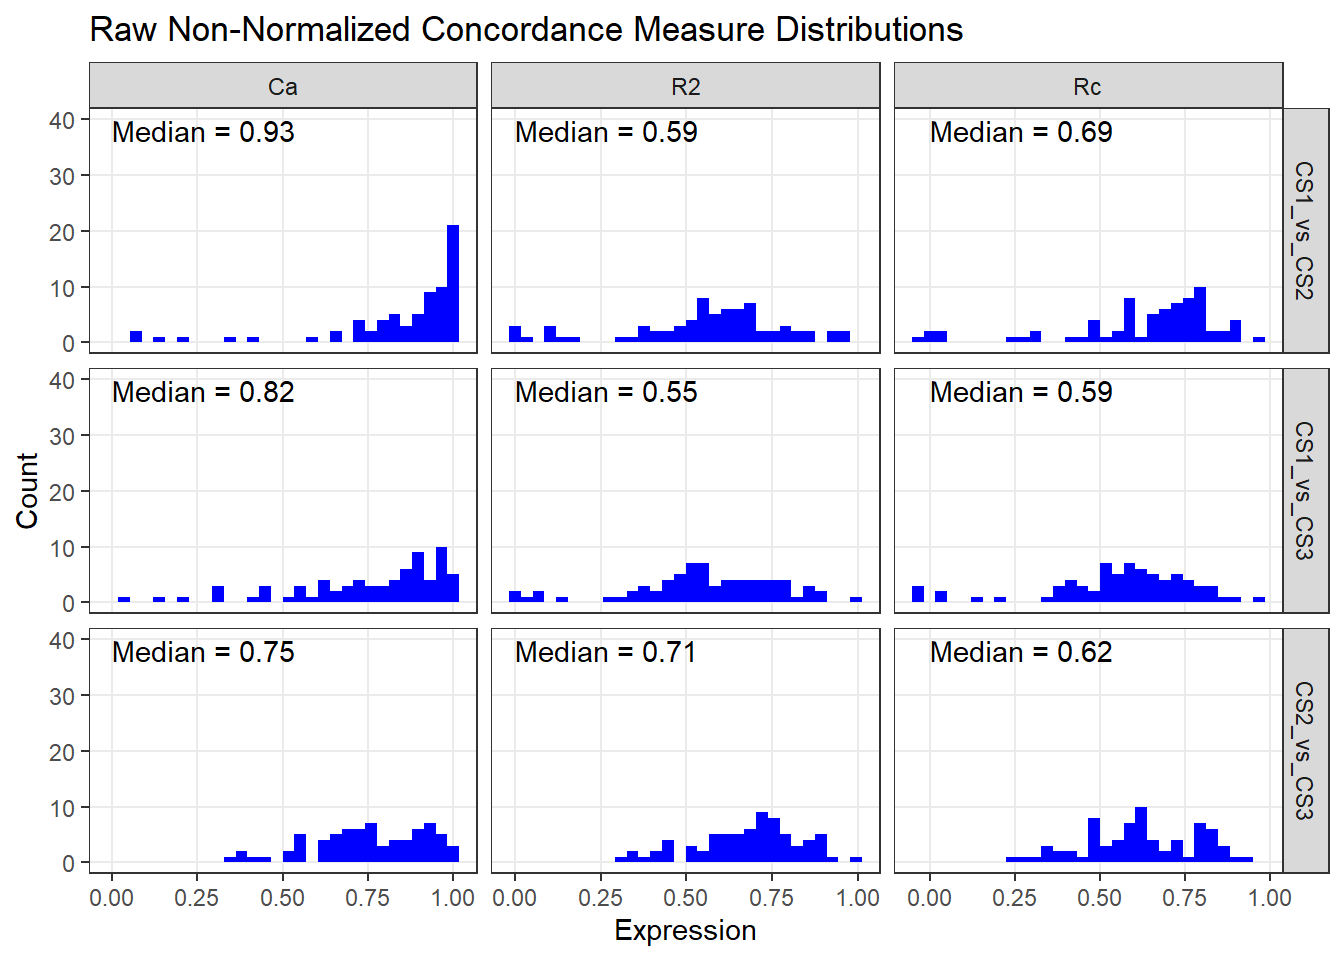
\includegraphics{OV_Histotypes_RSF_files/figure-latex/cc-raw-1} \end{center}

\begin{center}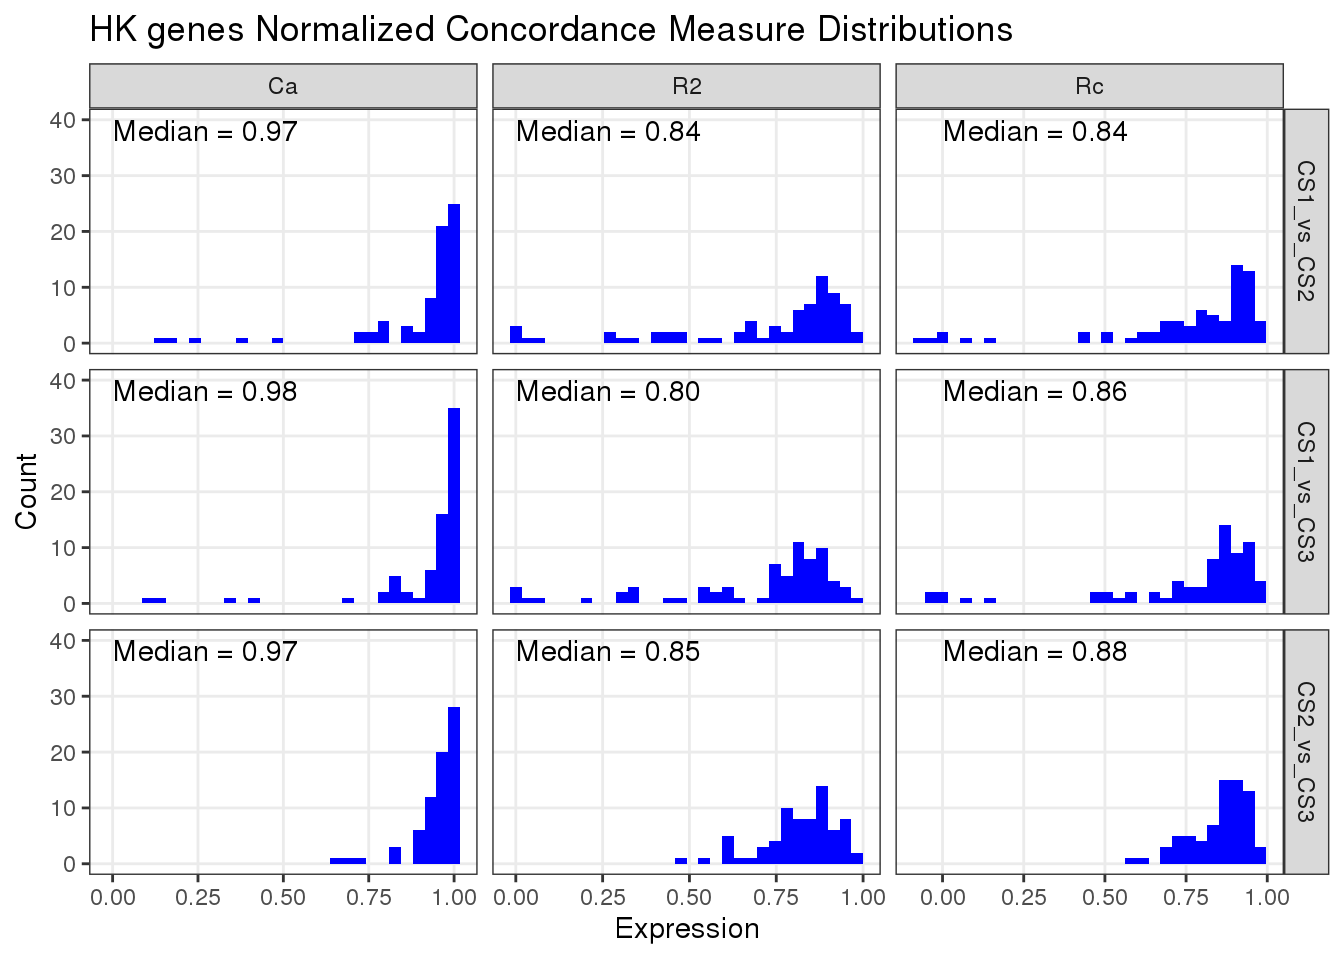
\includegraphics{OV_Histotypes_RSF_files/figure-latex/cc-hknorm-1} \end{center}

\hypertarget{common-samples-method-1}{%
\subsection{Common Samples Method}\label{common-samples-method-1}}

We employ a new normalization technique using randomly selected samples common to all three CodeSets with a uniform distribution of histotypes as the reference dataset. The number of randomly selected samples ranges from 1-3 per histotype. Hence, the reference dataset has either 5, 10, or 15 samples and we validate on the remaining. Note that ottaID duplicates are collapsed by mean averaging the gene expression. There are n=72 common samples.

CodeSets 1 and 2 are calibrated to CodeSet3 as follows:

\begin{itemize}
\tightlist
\item
  \texttt{X\^{}1(norm)\ =\ X\^{}1\ -\ R\^{}1\ +\ R\^{}3}~\\
\item
  \texttt{X\^{}2(norm)\ =\ X\^{}2\ -\ R\^{}2\ +\ R\^{}3}~\\
\item
  \texttt{X\^{}3(norm)\ =\ X\^{}3}
\end{itemize}

\hypertarget{random3}{%
\subsubsection{Random3}\label{random3}}

Randomly choose 3 samples from each of the 5 histotypes as the reference set (n=15). The rest are validated.

\begin{figure}[H]

{\centering 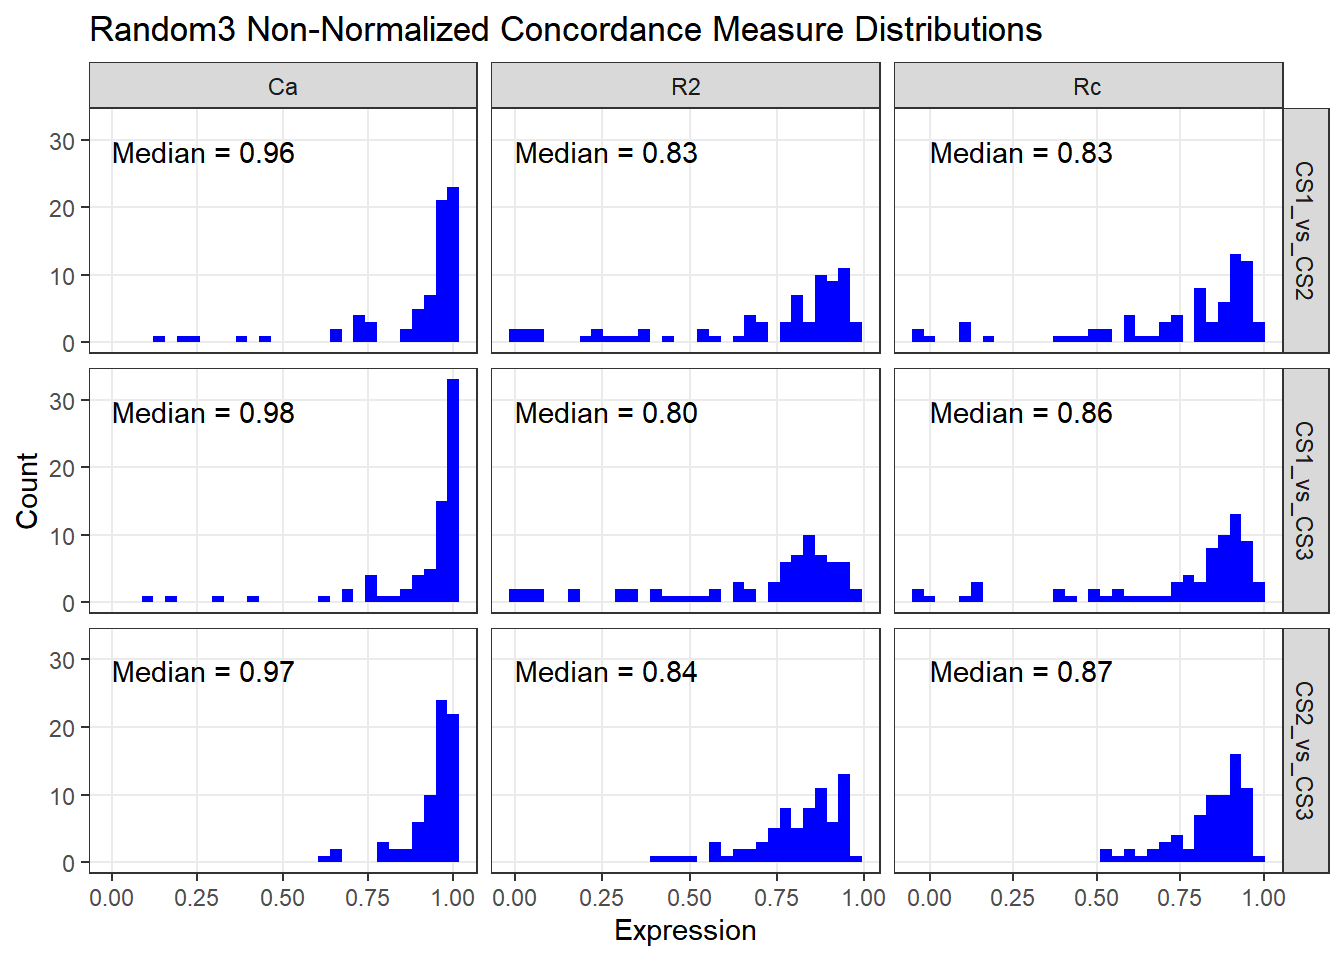
\includegraphics{OV_Histotypes_RSF_files/figure-latex/cc-non3-1} 

}

\caption{Random3 Non-Normalized Concordance Measure Distributions}\label{fig:cc-non3}
\end{figure}

\begin{figure}[H]

{\centering 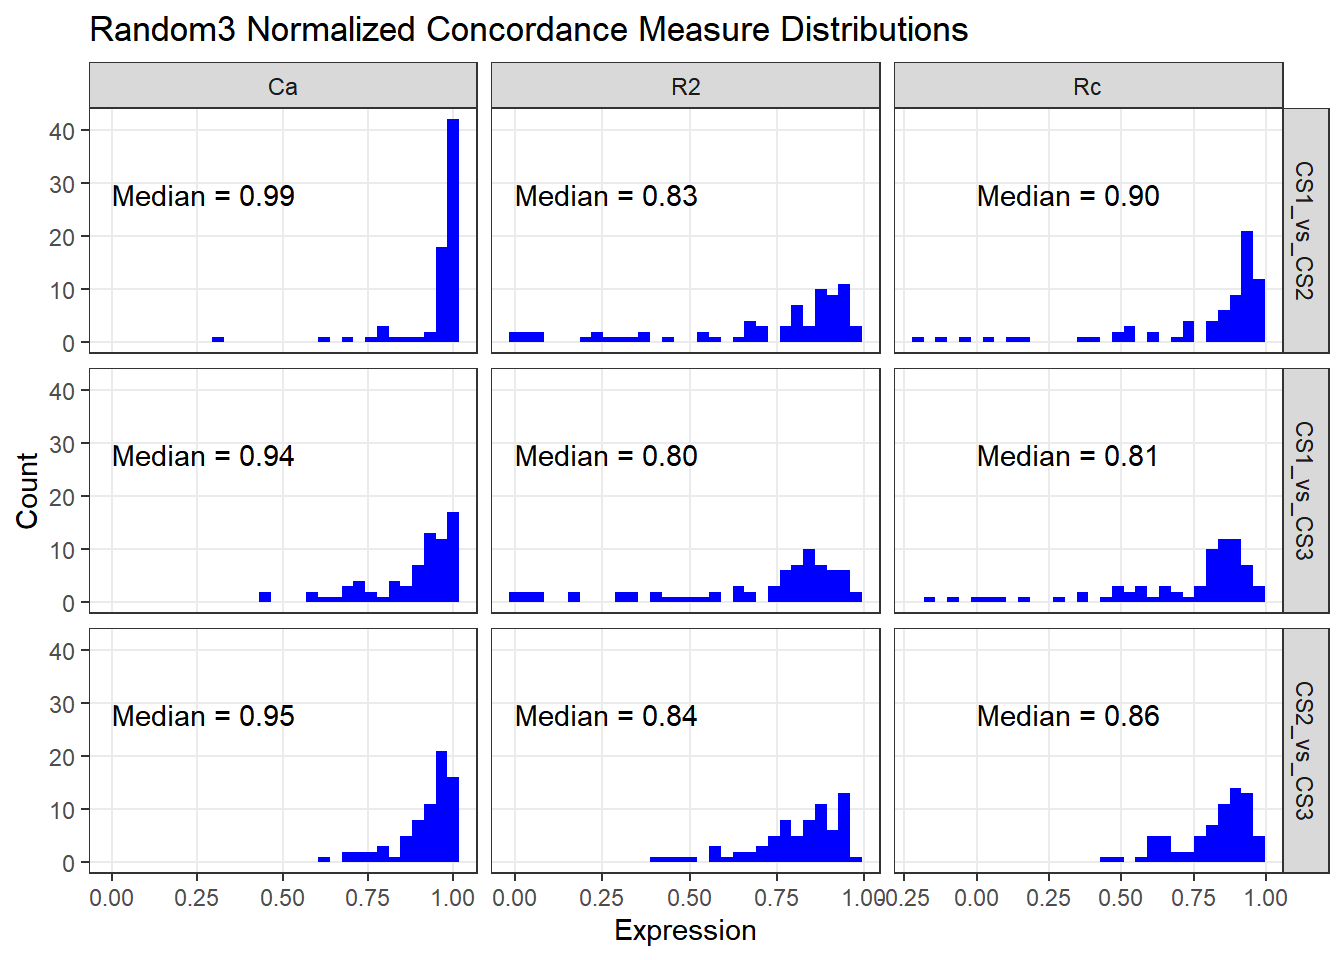
\includegraphics{OV_Histotypes_RSF_files/figure-latex/cc-rand3-1} 

}

\caption{Random3 Normalized Concordance Measure Distributions}\label{fig:cc-rand3}
\end{figure}

\hypertarget{random2}{%
\subsubsection{Random2}\label{random2}}

Randomly choose 2 samples from each of the 5 histotypes as the reference set (n=10). The rest are validated.

\begin{figure}[H]

{\centering 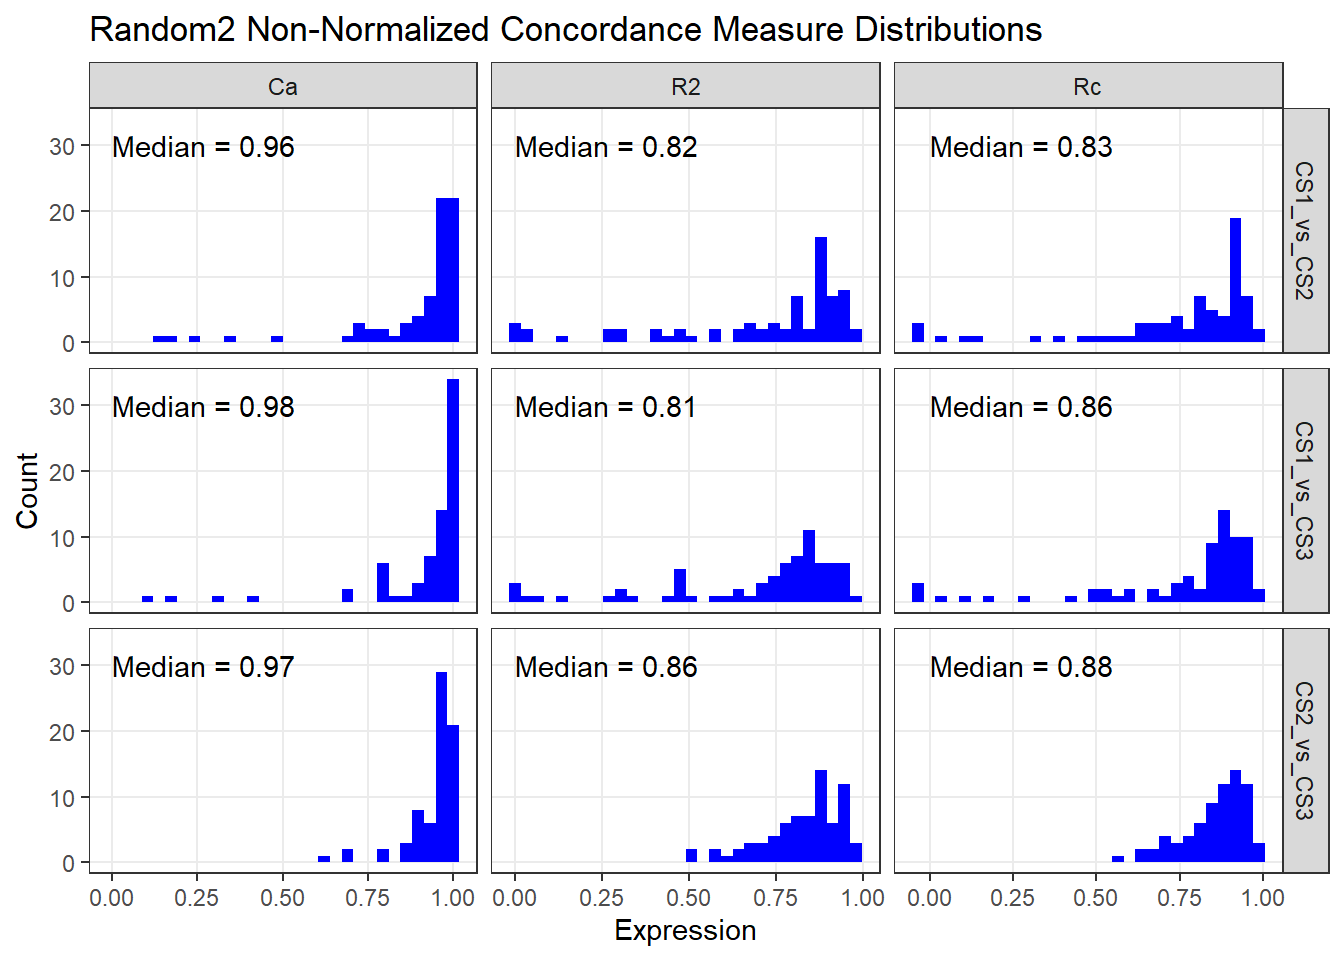
\includegraphics{OV_Histotypes_RSF_files/figure-latex/cc-non2-1} 

}

\caption{Random2 Non-Normalized Concordance Measure Distributions}\label{fig:cc-non2}
\end{figure}

\begin{figure}[H]

{\centering 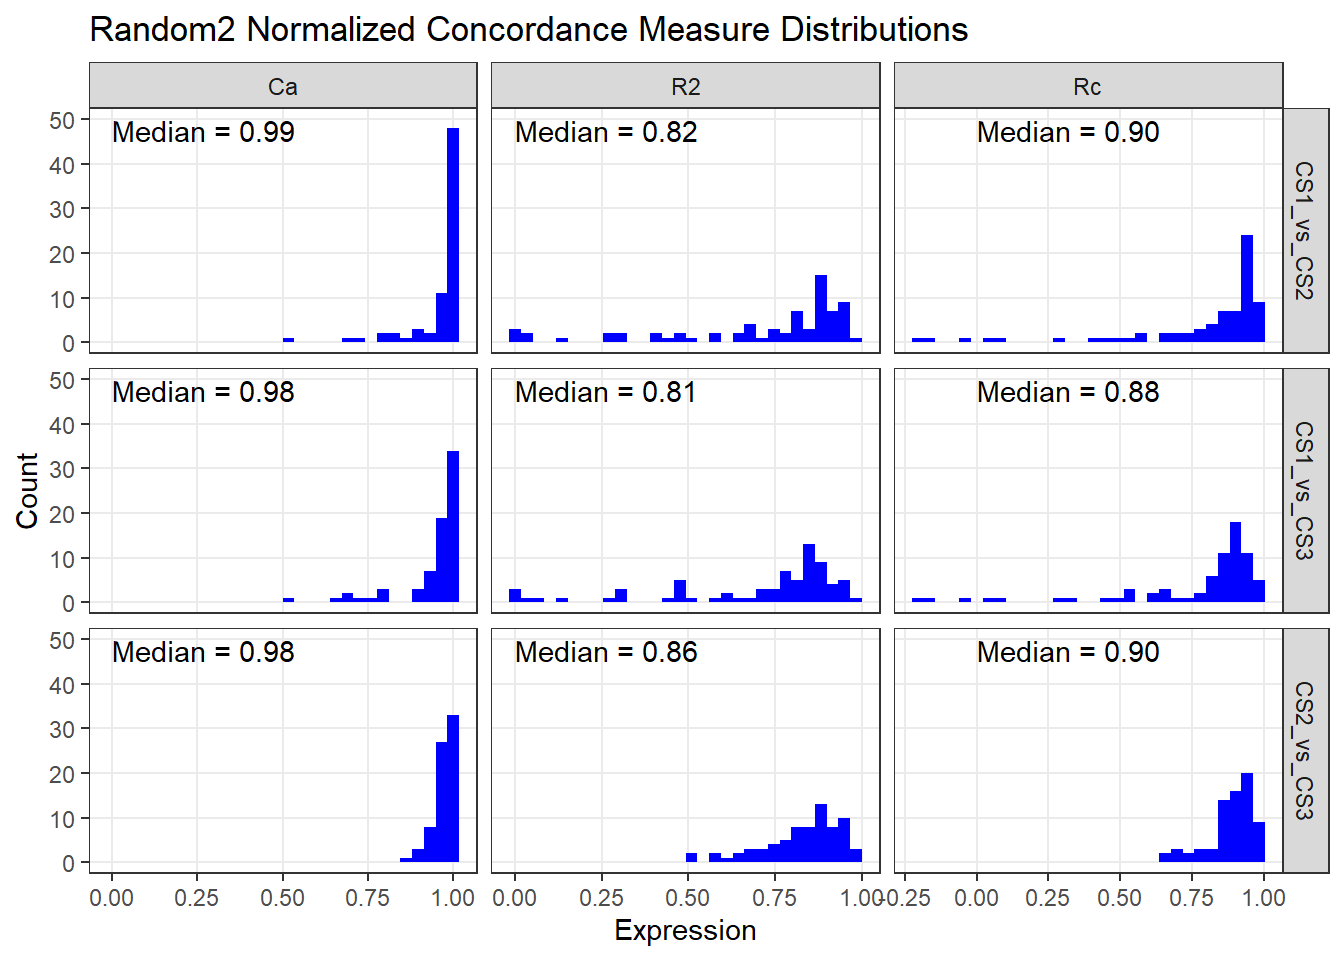
\includegraphics{OV_Histotypes_RSF_files/figure-latex/cc-rand2-1} 

}

\caption{Random2 Normalized Concordance Measure Distributions}\label{fig:cc-rand2}
\end{figure}

\hypertarget{random1}{%
\subsubsection{Random1}\label{random1}}

Randomly choose 1 sample from each of the 5 histotypes as the reference set (n=5). The rest are validated.

\begin{figure}[H]

{\centering 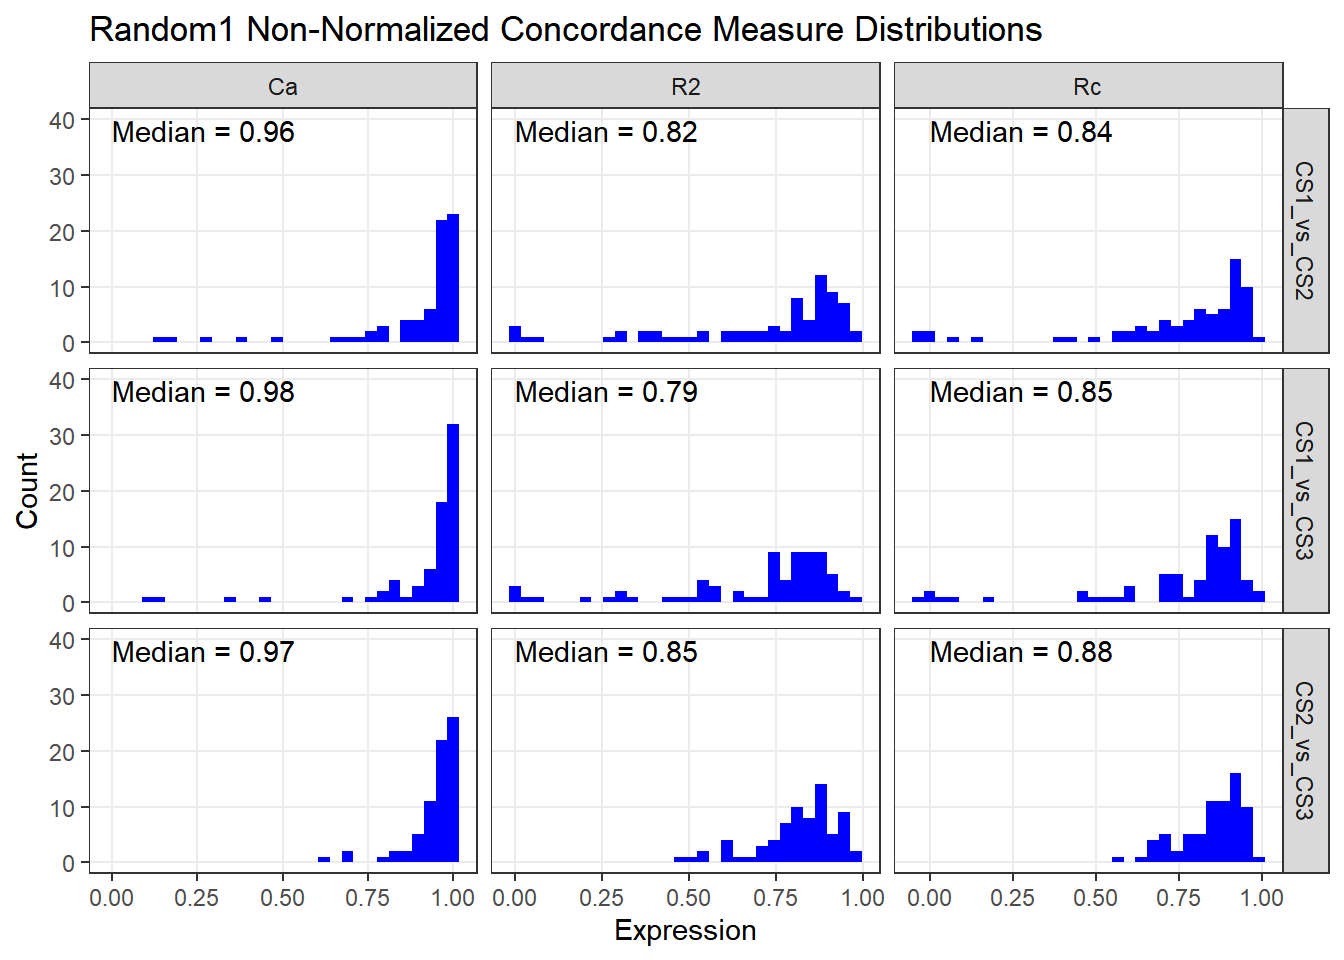
\includegraphics{OV_Histotypes_RSF_files/figure-latex/cc-non1-1} 

}

\caption{Random1 Non-Normalized Concordance Measure Distributions}\label{fig:cc-non1}
\end{figure}

\begin{figure}[H]

{\centering 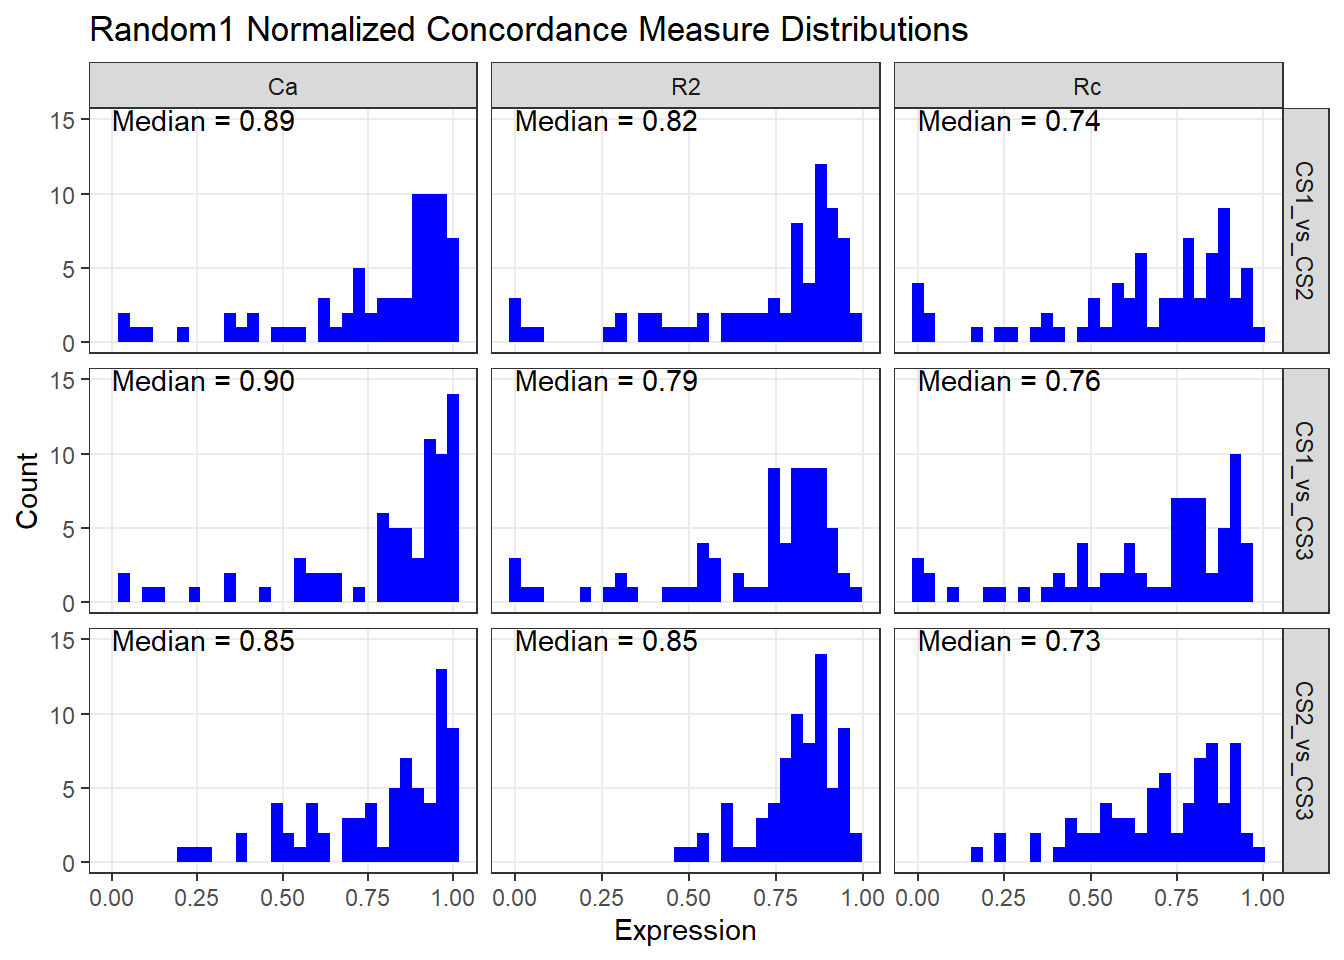
\includegraphics{OV_Histotypes_RSF_files/figure-latex/cc-rand1-1} 

}

\caption{Random1 Normalized Concordance Measure Distributions}\label{fig:cc-rand1}
\end{figure}

In Tables \ref{tab:rand1-cs1-vs-cs3} and \ref{tab:rand1-cs2-vs-cs3}, we calculate the concordance measures for CS1 vs.~CS3 and CS2 cs. CS3, respectively. The measures are calculated for both non-normalized and normalized datasets (CS1, CS2), and split by histotype.

\begin{table}

\caption{\label{tab:rand1-cs1-vs-cs3}Random1 CS1 vs. CS3 Median Concordance Measures by Histotypes}
\centering
\begin{tabular}[t]{l|r|r|r|r|r|r}
\hline
hist & R2-Non & Ca-Non & Rc-Non & R2-Norm & Ca-Norm & Rc-Norm\\
\hline
CCOC & 1.00 & 0.29 & 0.12 & 1.00 & 0.29 & 0.10\\
\hline
ENOC & 1.00 & 0.54 & 0.54 & 1.00 & 0.62 & 0.62\\
\hline
HGSC & 0.79 & 0.98 & 0.85 & 0.79 & 0.97 & 0.87\\
\hline
LGSC & 0.96 & 0.89 & 0.82 & 0.96 & 0.91 & 0.87\\
\hline
MUC & 0.77 & 0.86 & 0.68 & 0.77 & 0.81 & 0.63\\
\hline
\end{tabular}
\end{table}

\begin{table}

\caption{\label{tab:rand1-cs2-vs-cs3}Random1 CS2 vs. CS3 Median Concordance Measures by Histotypes}
\centering
\begin{tabular}[t]{l|r|r|r|r|r|r}
\hline
hist & R2-Non & Ca-Non & Rc-Non & R2-Norm & Ca-Norm & Rc-Norm\\
\hline
CCOC & 1.00 & 0.23 & 0.08 & 1.00 & 0.27 & 0.16\\
\hline
ENOC & 1.00 & 0.63 & 0.61 & 1.00 & 0.61 & 0.57\\
\hline
HGSC & 0.83 & 0.96 & 0.86 & 0.83 & 0.98 & 0.89\\
\hline
LGSC & 0.98 & 0.92 & 0.90 & 0.98 & 0.95 & 0.93\\
\hline
MUC & 0.68 & 0.77 & 0.55 & 0.68 & 0.86 & 0.61\\
\hline
\end{tabular}
\end{table}

Because Random1 is a random selection of reference samples, we want to assess the variability of the concordance measures by repeating Random1 on different selections and observing the distribution of the medians.

\begin{figure}[H]

{\centering 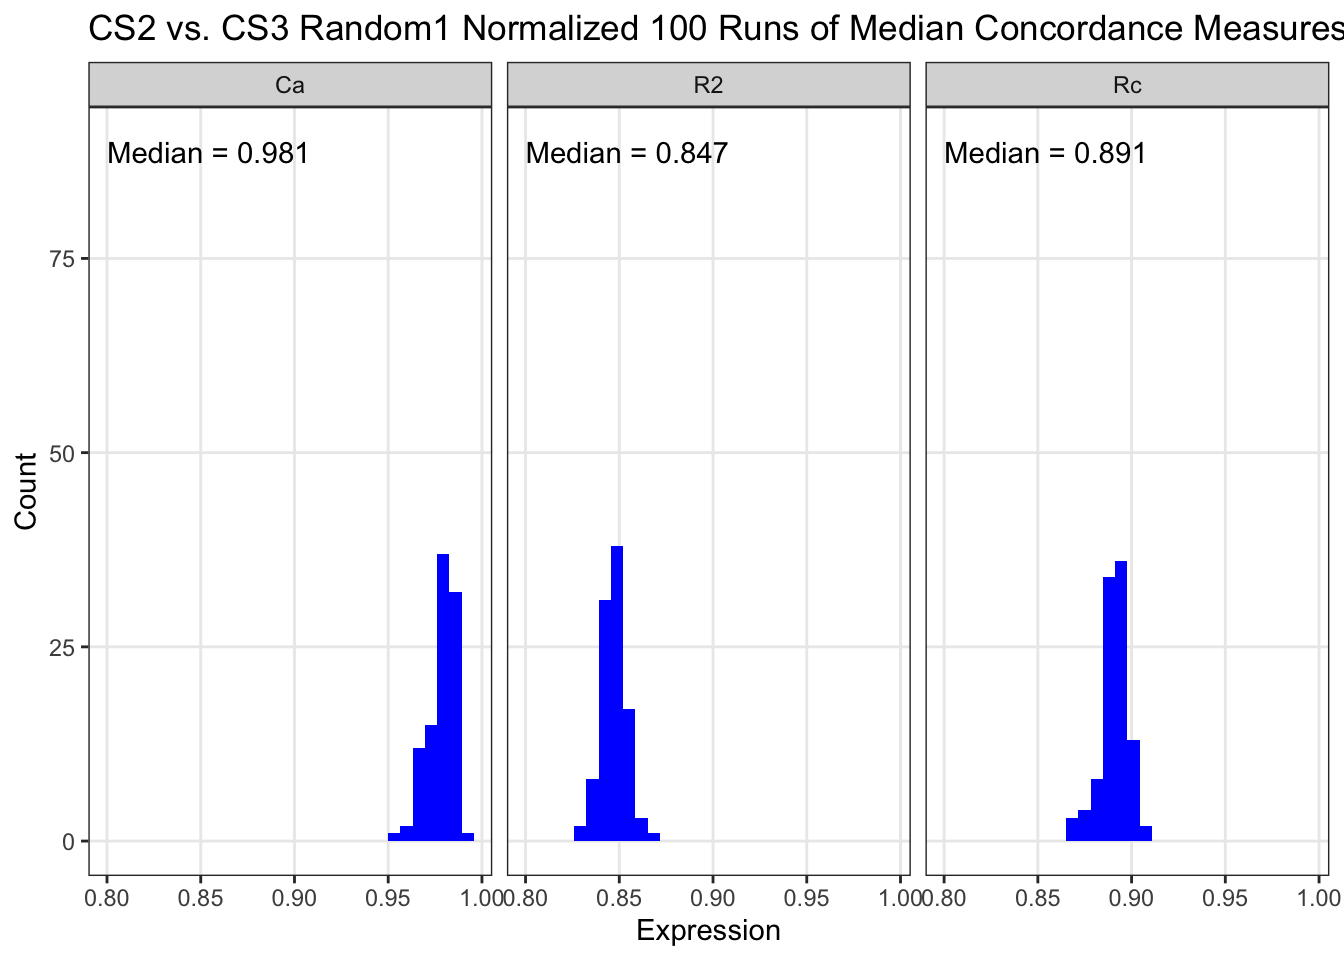
\includegraphics{OV_Histotypes_RSF_files/figure-latex/cc-rand1-cs23-meds-1} 

}

\caption{CS2 vs. CS3 Random1 Normalized 100 Runs of Median Concordance Measures}\label{fig:cc-rand1-cs23-meds}
\end{figure}

\begin{table}

\caption{\label{tab:metrics-summ-cs23}CS2 vs CS3 Random1 Normalized 100 Runs of Summary Concordance Measures}
\centering
\begin{tabular}[t]{l|r|r|r|r}
\hline
Metric & Min & Median & Max & SD\\
\hline
Ca & 0.956 & 0.981 & 0.989 & 0.007\\
\hline
R2 & 0.830 & 0.847 & 0.870 & 0.007\\
\hline
Rc & 0.867 & 0.891 & 0.907 & 0.008\\
\hline
\end{tabular}
\end{table}

\hypertarget{random3-hgsc}{%
\subsubsection{Random3 HGSC}\label{random3-hgsc}}

Randomly choose n=3 HGSC samples as the reference set, and use the rest as validation. This was tried in lieu of the fact that some non-HGSC histotypes have at most n=3 samples in total, so using Random3 or even Random2 would leave no samples remaining in the validation set for these histotypes.

\begin{figure}[H]

{\centering 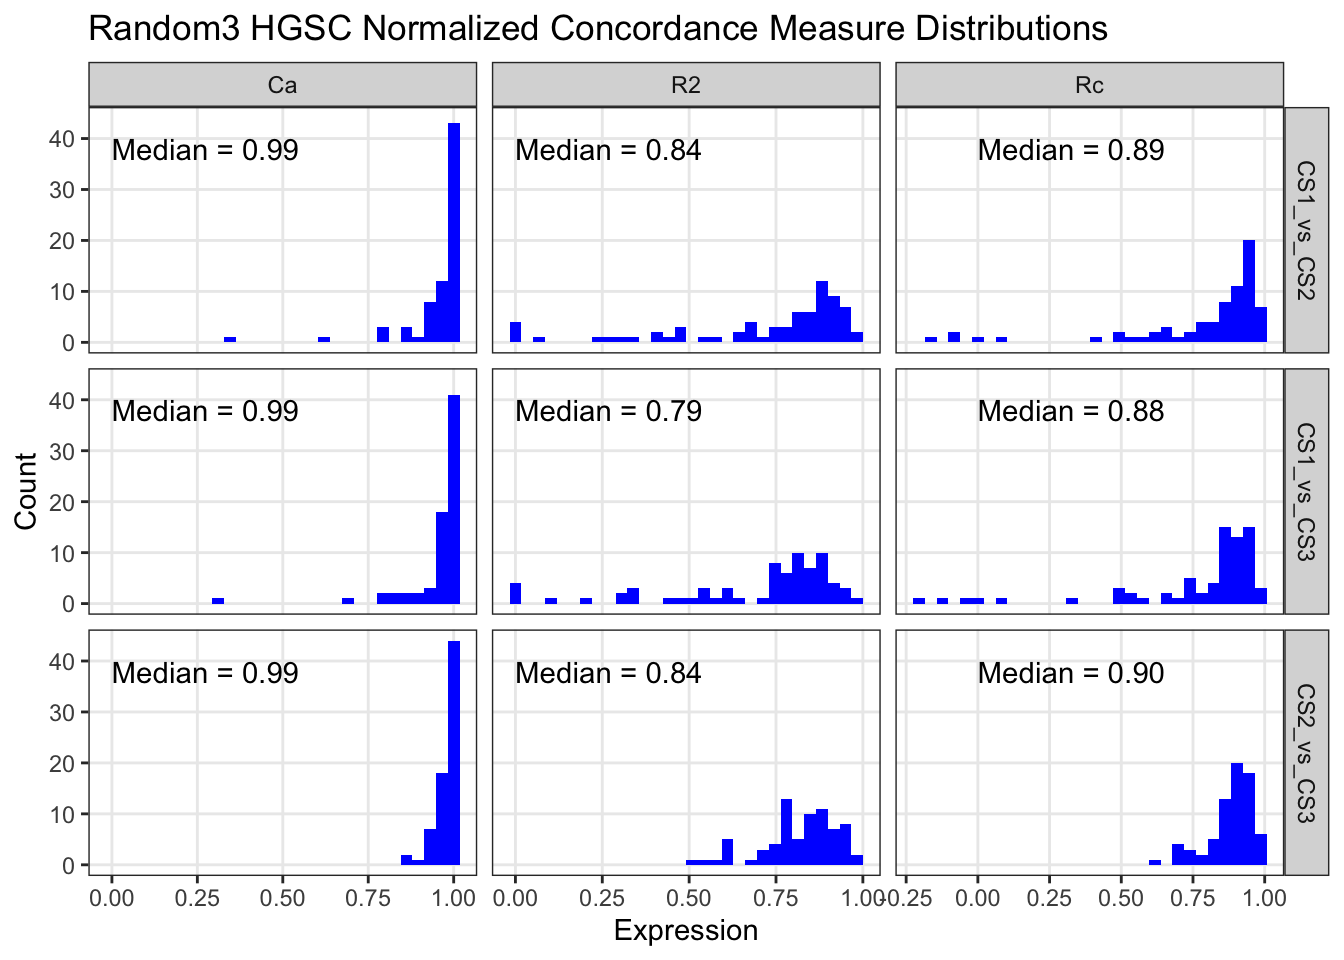
\includegraphics{OV_Histotypes_RSF_files/figure-latex/cc-rand-1} 

}

\caption{Random3 HGSC Normalized Concordance Measure Distributions}\label{fig:cc-rand}
\end{figure}

In Tables \ref{tab:rand3-hgsc-cs1-vs-cs3} and \ref{tab:rand3-hgsc-cs2-vs-cs3}, we calculate the concordance measures for CS1 vs.~CS3 and CS2 cs. CS3, respectively. The measures are calculated for both non-normalized and normalized datasets (CS1, CS2), and split by histotype.

\begin{table}

\caption{\label{tab:rand3-hgsc-cs1-vs-cs3}Random3 HGSC CS1 vs. CS3 Median Concordance Measures by Histotypes}
\centering
\begin{tabular}[t]{l|r|r|r|r|r|r}
\hline
hist & R2-Non & Ca-Non & Rc-Non & R2-Norm & Ca-Norm & Rc-Norm\\
\hline
CCOC & 0.62 & 0.62 & 0.32 & 0.62 & 0.68 & 0.27\\
\hline
ENOC & 0.88 & 0.76 & 0.66 & 0.88 & 0.77 & 0.70\\
\hline
HGSC & 0.77 & 0.97 & 0.85 & 0.77 & 0.99 & 0.87\\
\hline
LGSC & 0.94 & 0.85 & 0.80 & 0.94 & 0.90 & 0.84\\
\hline
MUC & 0.74 & 0.92 & 0.72 & 0.74 & 0.93 & 0.78\\
\hline
\end{tabular}
\end{table}

\begin{table}

\caption{\label{tab:rand3-hgsc-cs2-vs-cs3}Random3 HGSC CS2 vs. CS3 Median Concordance Measures by Histotypes}
\centering
\begin{tabular}[t]{l|r|r|r|r|r|r}
\hline
hist & R2-Non & Ca-Non & Rc-Non & R2-Norm & Ca-Norm & Rc-Norm\\
\hline
CCOC & 0.66 & 0.56 & 0.35 & 0.66 & 0.59 & 0.42\\
\hline
ENOC & 0.85 & 0.76 & 0.66 & 0.85 & 0.85 & 0.76\\
\hline
HGSC & 0.82 & 0.96 & 0.86 & 0.82 & 0.99 & 0.90\\
\hline
LGSC & 0.97 & 0.95 & 0.92 & 0.97 & 0.92 & 0.90\\
\hline
MUC & 0.74 & 0.89 & 0.72 & 0.74 & 0.93 & 0.72\\
\hline
\end{tabular}
\end{table}

\hypertarget{random1-for-sites}{%
\subsubsection{Random1 for Sites}\label{random1-for-sites}}

We use the Random1 method to normalize CS3-USC and CS3-AOC to CS3-VAN. There aren't enough samples in the USC and AOC cohorts to perform Random2 or Random3.

\begin{figure}[H]

{\centering 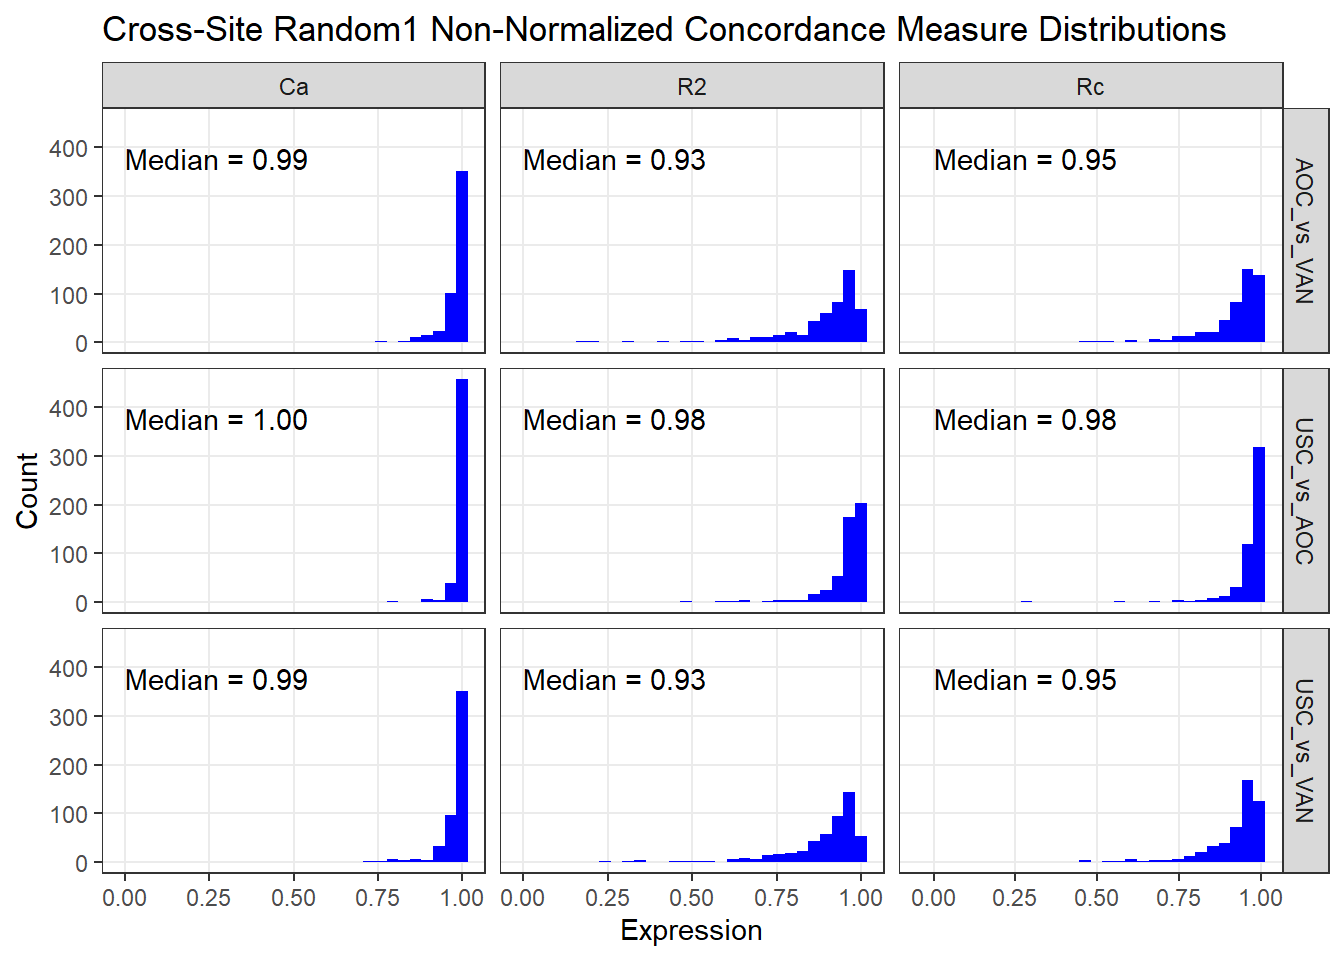
\includegraphics{OV_Histotypes_RSF_files/figure-latex/cc-site-non1-1} 

}

\caption{Cross-Site Random1 Non-Normalized Concordance Measure Distributions}\label{fig:cc-site-non1}
\end{figure}

\begin{center}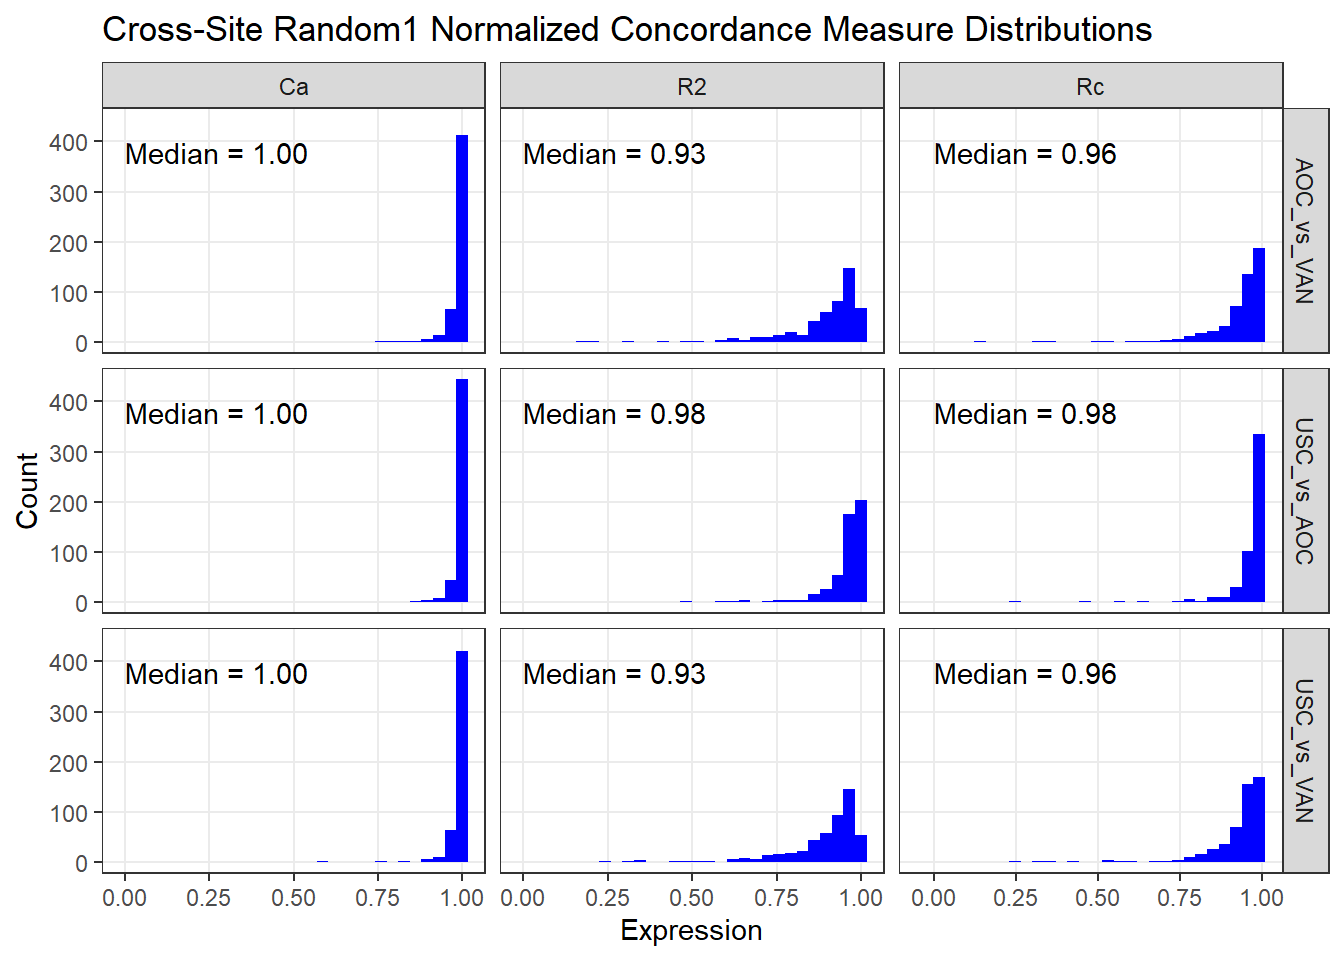
\includegraphics{OV_Histotypes_RSF_files/figure-latex/cc-site-rand1-1} \end{center}

\hypertarget{pools-method-1}{%
\subsection{Pools Method}\label{pools-method-1}}

\hypertarget{cs2-vs.-cs3}{%
\subsubsection{CS2 vs.~CS3}\label{cs2-vs.-cs3}}

CodeSet2 contains 12 ref pool samples (Pool 1 = 4, Pool 2 = 4, Pool 3 = 4). CodeSet3 contains 22 ref pool samples (Pool 1 = 12, Pool 2 = 5, Pool 3 = 5). n=84 common samples.

CodeSet2 is calibrated to CodeSet3 as follows:\\
\texttt{X\^{}2(norm)\ =\ X\^{}2\ -\ R\^{}2\ +\ R\^{}3}~\\
\texttt{X\^{}3(norm)\ =\ X\^{}3}

\begin{figure}[H]

{\centering 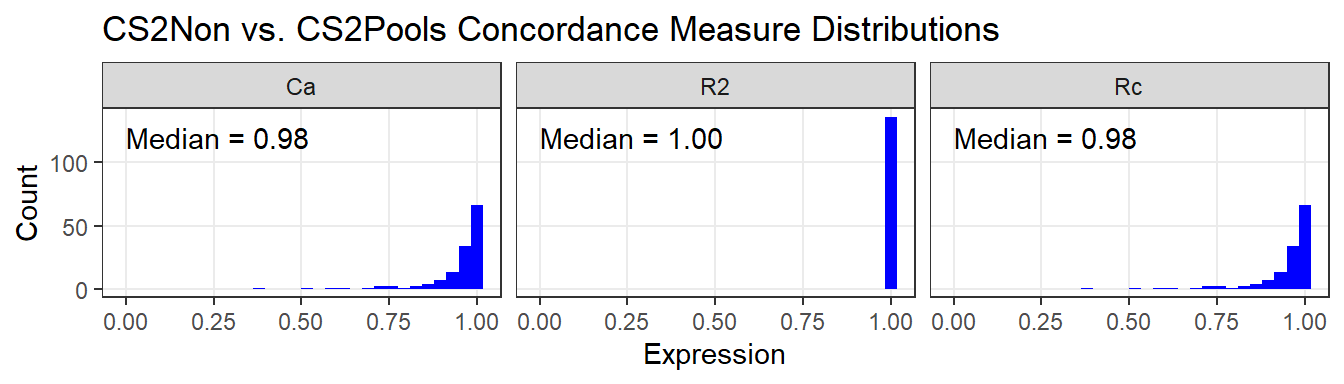
\includegraphics{OV_Histotypes_RSF_files/figure-latex/cc-cs2non-vs-cs2pools-1} 

}

\caption{CS2Non vs. CS2Pools Concordance Measure Distributions}\label{fig:cc-cs2non-vs-cs2pools}
\end{figure}

\begin{figure}[H]

{\centering 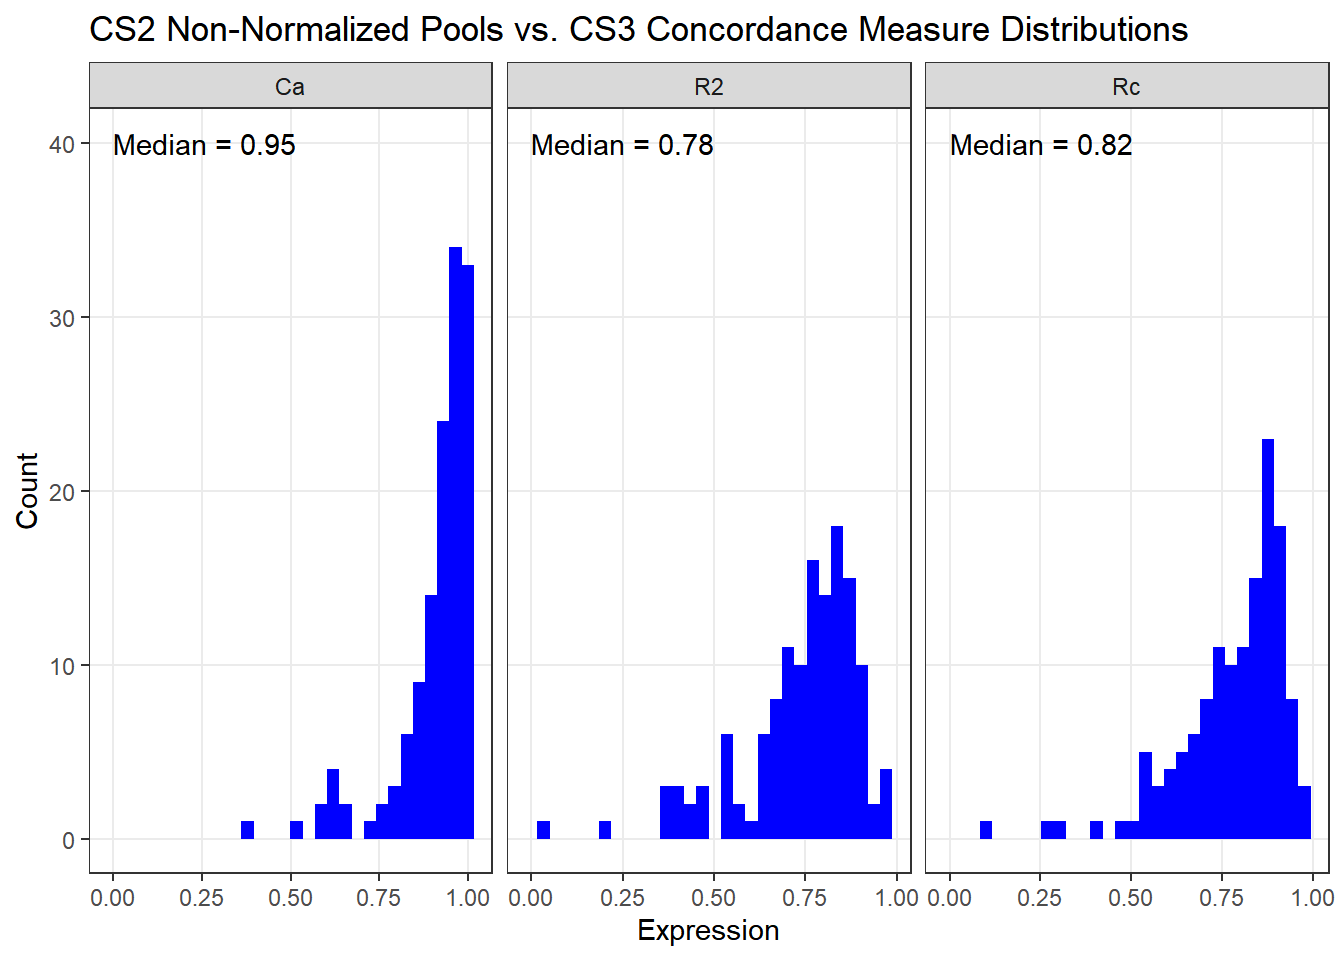
\includegraphics{OV_Histotypes_RSF_files/figure-latex/cc-cs2non-vs-cs3-1} 

}

\caption{CS2 Non-Normalized Pools vs. CS3 Concordance Measure Distributions}\label{fig:cc-cs2non-vs-cs3}
\end{figure}

\begin{figure}[H]

{\centering 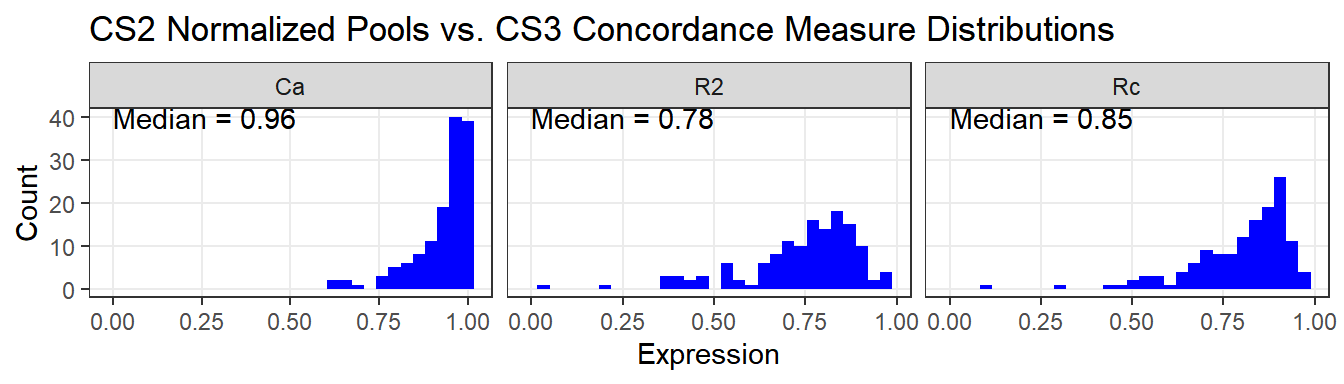
\includegraphics{OV_Histotypes_RSF_files/figure-latex/cc-cs2pools-vs-cs3-1} 

}

\caption{CS2 Normalized Pools vs. CS3 Concordance Measure Distributions}\label{fig:cc-cs2pools-vs-cs3}
\end{figure}

\begin{table}

\caption{\label{tab:pools-cs2non-vs-cs3}Pools Non-Normalized CS2 vs. CS3 Median Concordance Measures by Histotypes}
\centering
\begin{tabular}[t]{l|r|r|r}
\hline
hist & R2 & Ca & Rc\\
\hline
CCOC & 0.66 & 0.53 & 0.26\\
\hline
ENOC & 0.88 & 0.74 & 0.63\\
\hline
HGSC & 0.77 & 0.94 & 0.80\\
\hline
LGSC & 0.98 & 0.95 & 0.92\\
\hline
MUC & 0.74 & 0.86 & 0.68\\
\hline
\end{tabular}
\end{table}

\begin{table}

\caption{\label{tab:pools-cs2norm-vs-cs3}Pools Normalized CS2 vs. CS3 Median Concordance Measures by Histotypes}
\centering
\begin{tabular}[t]{l|r|r|r}
\hline
hist & R2 & Ca & Rc\\
\hline
CCOC & 0.66 & 0.60 & 0.32\\
\hline
ENOC & 0.88 & 0.76 & 0.68\\
\hline
HGSC & 0.77 & 0.94 & 0.81\\
\hline
LGSC & 0.98 & 0.95 & 0.93\\
\hline
MUC & 0.74 & 0.91 & 0.71\\
\hline
\end{tabular}
\end{table}

\hypertarget{usc-vs.-van}{%
\subsubsection{USC vs.~VAN}\label{usc-vs.-van}}

In CodeSet 3, we normalize the USC and AOC cohorts to the VAN cohort which is used as the reference dataset.

\begin{figure}[H]

{\centering 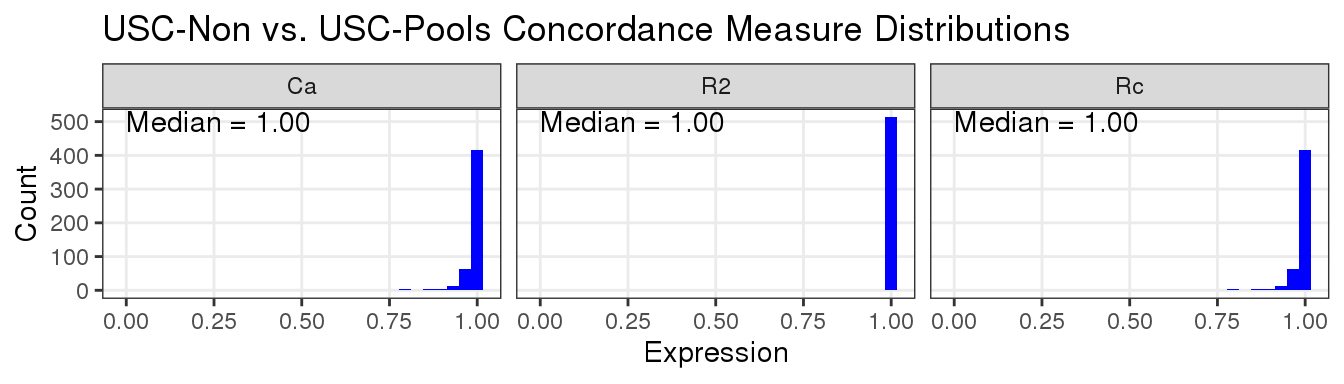
\includegraphics{OV_Histotypes_RSF_files/figure-latex/cc-uscnon-vs-uscpools-1} 

}

\caption{USC-Non vs. USC-Pools Concordance Measure Distributions}\label{fig:cc-uscnon-vs-uscpools}
\end{figure}

\begin{figure}[H]

{\centering 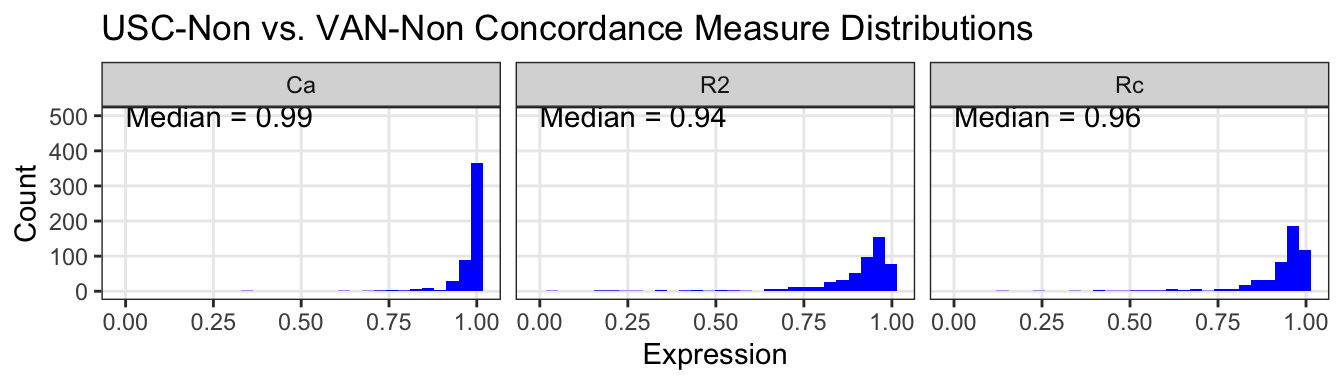
\includegraphics{OV_Histotypes_RSF_files/figure-latex/cc-uscnon-vs-vannon-1} 

}

\caption{USC-Non vs. VAN-Non Concordance Measure Distributions}\label{fig:cc-uscnon-vs-vannon}
\end{figure}

\begin{figure}[H]

{\centering 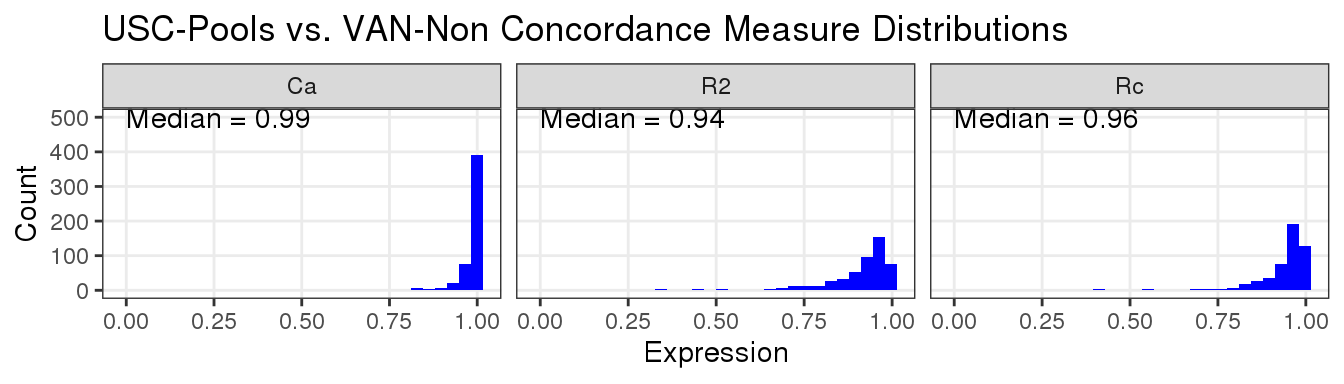
\includegraphics{OV_Histotypes_RSF_files/figure-latex/cc-uscpools-vs-vannon-1} 

}

\caption{USC-Pools vs. VAN-Non Concordance Measure Distributions}\label{fig:cc-uscpools-vs-vannon}
\end{figure}

\begin{figure}[H]

{\centering 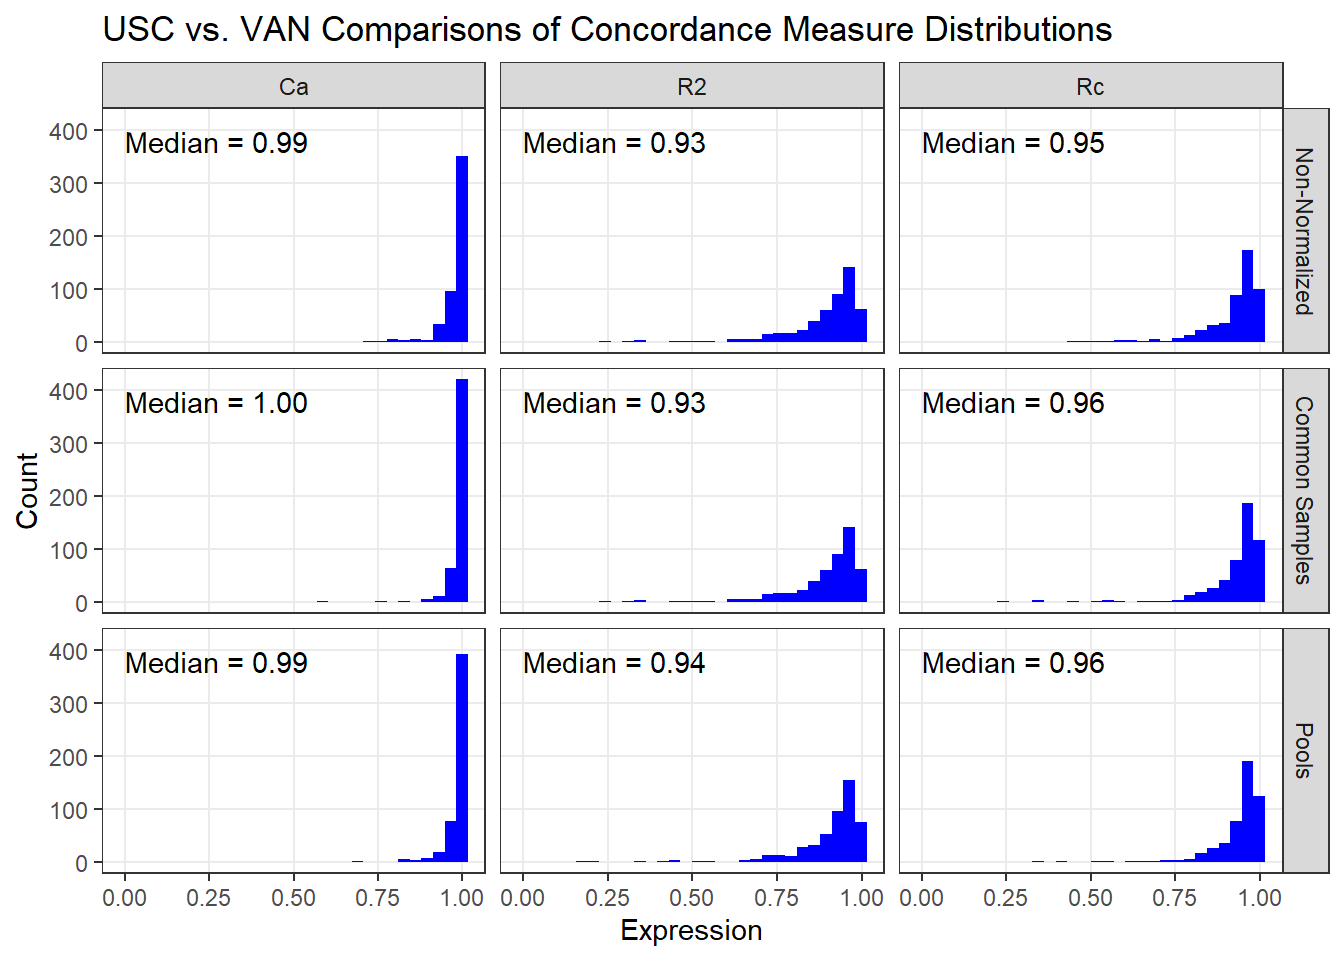
\includegraphics{OV_Histotypes_RSF_files/figure-latex/usc-vs-van-comps-1} 

}

\caption{USC vs. VAN Comparisons of Concordance Measure Distributions}\label{fig:usc-vs-van-comps}
\end{figure}

\hypertarget{aoc-vs.-van}{%
\subsubsection{AOC vs.~VAN}\label{aoc-vs.-van}}

\begin{figure}[H]

{\centering 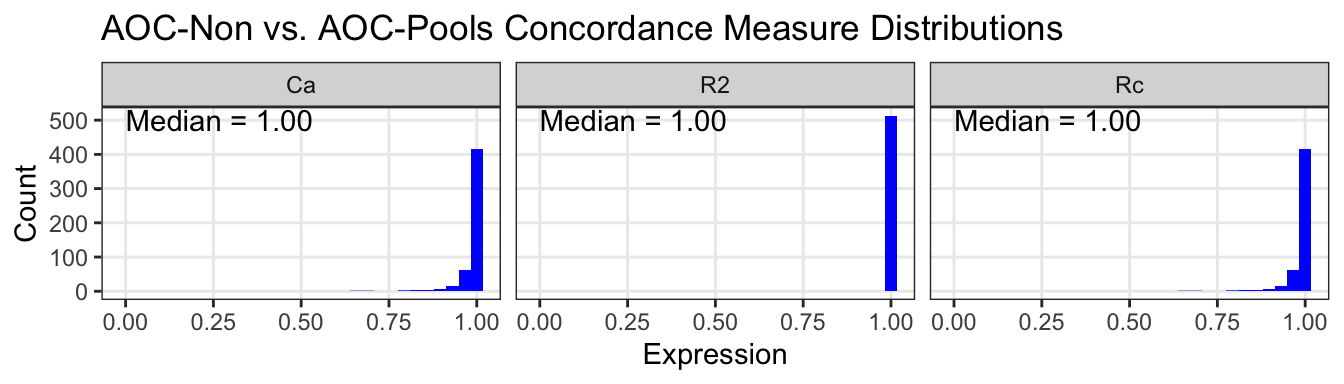
\includegraphics{OV_Histotypes_RSF_files/figure-latex/cc-aocnon-vs-aocpools-1} 

}

\caption{AOC-Non vs. AOC-Pools Concordance Measure Distributions}\label{fig:cc-aocnon-vs-aocpools}
\end{figure}

\begin{figure}[H]

{\centering 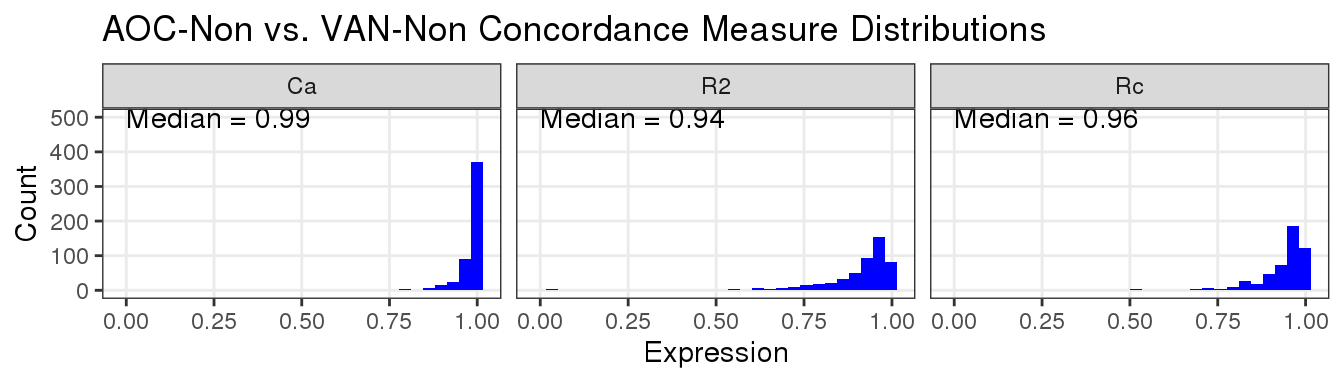
\includegraphics{OV_Histotypes_RSF_files/figure-latex/cc-aocnon-vs-vannon-1} 

}

\caption{AOC-Non vs. VAN-Non Concordance Measure Distributions}\label{fig:cc-aocnon-vs-vannon}
\end{figure}

\begin{figure}[H]

{\centering 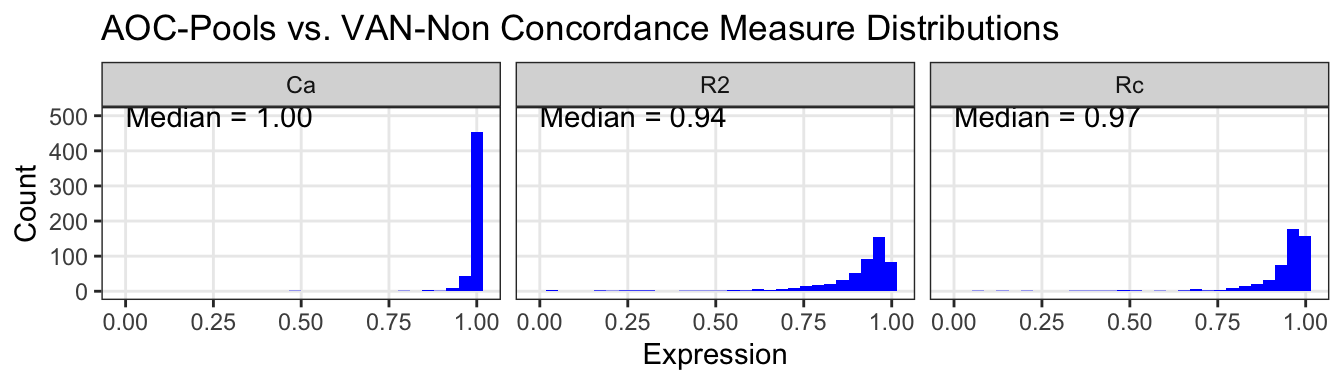
\includegraphics{OV_Histotypes_RSF_files/figure-latex/cc-aocpools-vs-vannon-1} 

}

\caption{AOC-Pools vs. VAN-Non Concordance Measure Distributions}\label{fig:cc-aocpools-vs-vannon}
\end{figure}

\begin{figure}[H]

{\centering 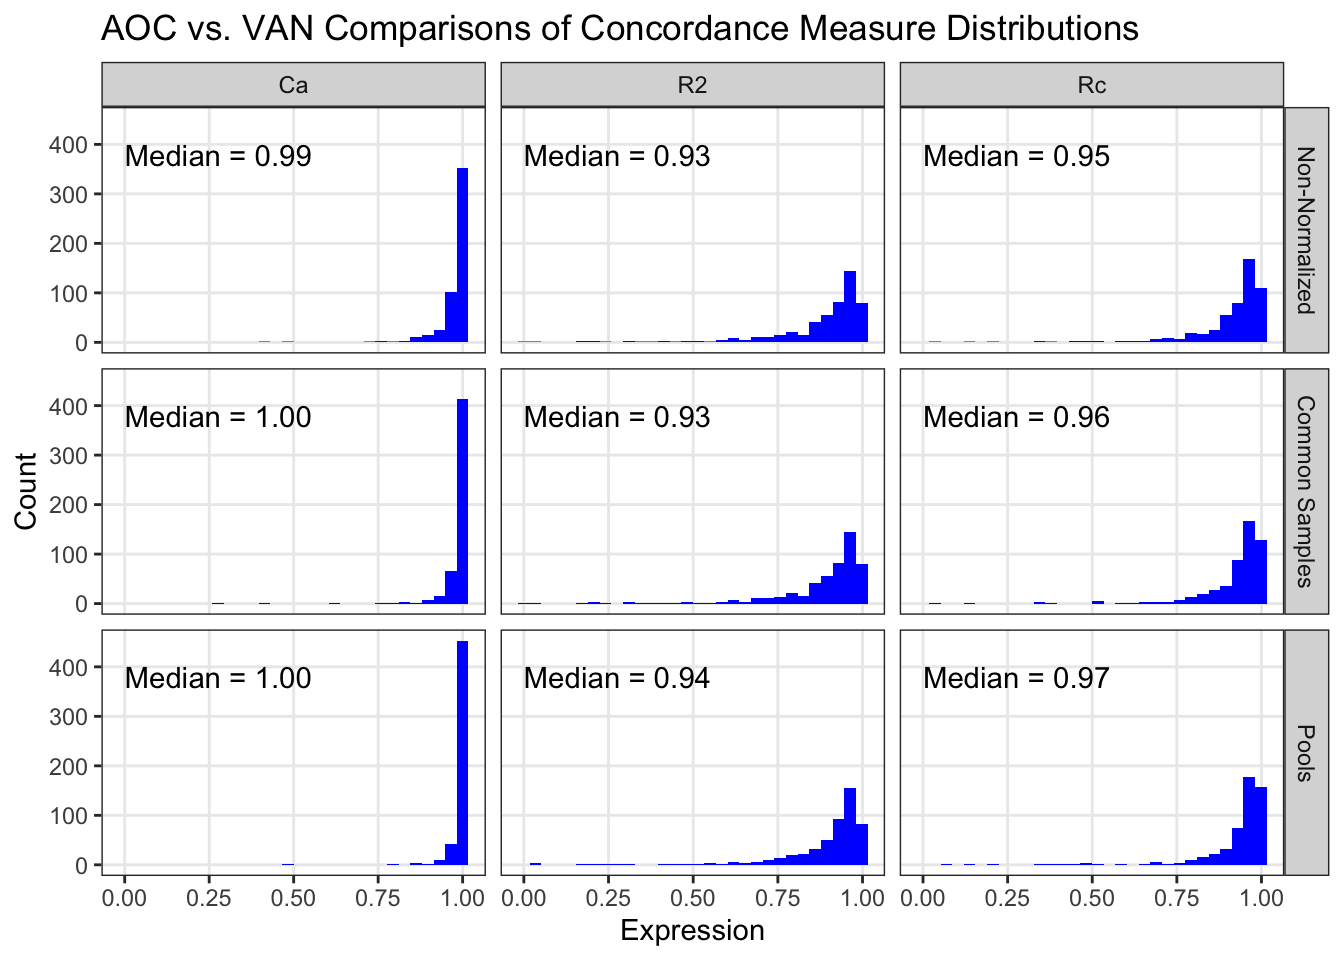
\includegraphics{OV_Histotypes_RSF_files/figure-latex/aoc-vs-van-comps-1} 

}

\caption{AOC vs. VAN Comparisons of Concordance Measure Distributions}\label{fig:aoc-vs-van-comps}
\end{figure}

\hypertarget{common-samples-vs.-pools-comparison}{%
\subsection{Common Samples vs.~Pools Comparison}\label{common-samples-vs.-pools-comparison}}

Since only CS2 and CS3 have pools, we make three comparisons between these two CodeSets:

\begin{itemize}
\tightlist
\item
  Non-Normalized
\item
  Common Samples Method
\item
  Pools Method
\end{itemize}

\begin{figure}[H]

{\centering 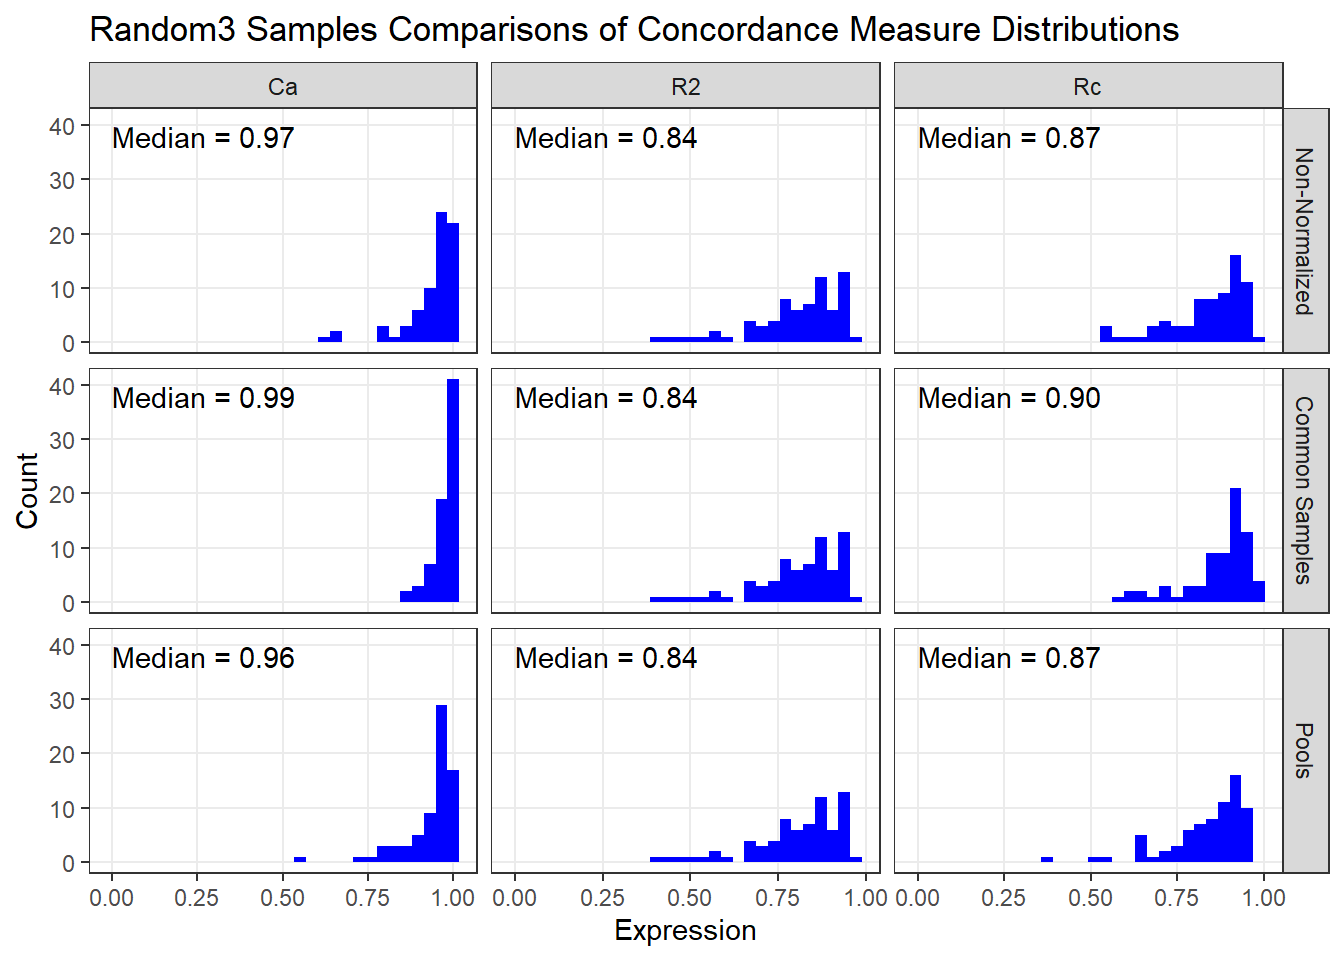
\includegraphics{OV_Histotypes_RSF_files/figure-latex/rand3-vs-pools-1} 

}

\caption{Random3 Samples Comparisons of Concordance Measure Distributions}\label{fig:rand3-vs-pools}
\end{figure}

\begin{table}

\caption{\label{tab:rand3-vs-pools-stats}Random3 Samples Comparisons Statistics by Histotypes}
\centering
\begin{tabular}[t]{l|r|r|r|r|r|r|r|r|r}
\hline
hist & R2-Non & Ca-Non & Rc-Non & R2-Common & Ca-Common & Rc-Common & R2-Pools & Ca-Pools & Rc-Pools\\
\hline
HGSC & 0.84 & 0.96 & 0.86 & 0.84 & 0.99 & 0.90 & 0.84 & 0.96 & 0.86\\
\hline
LGSC & NA & NA & NA & NA & NA & NA & NA & NA & NA\\
\hline
MUC & 1.00 & 0.49 & 0.44 & 1.00 & 0.62 & 0.52 & 1.00 & 0.46 & 0.42\\
\hline
\end{tabular}
\end{table}

\begin{figure}[H]

{\centering 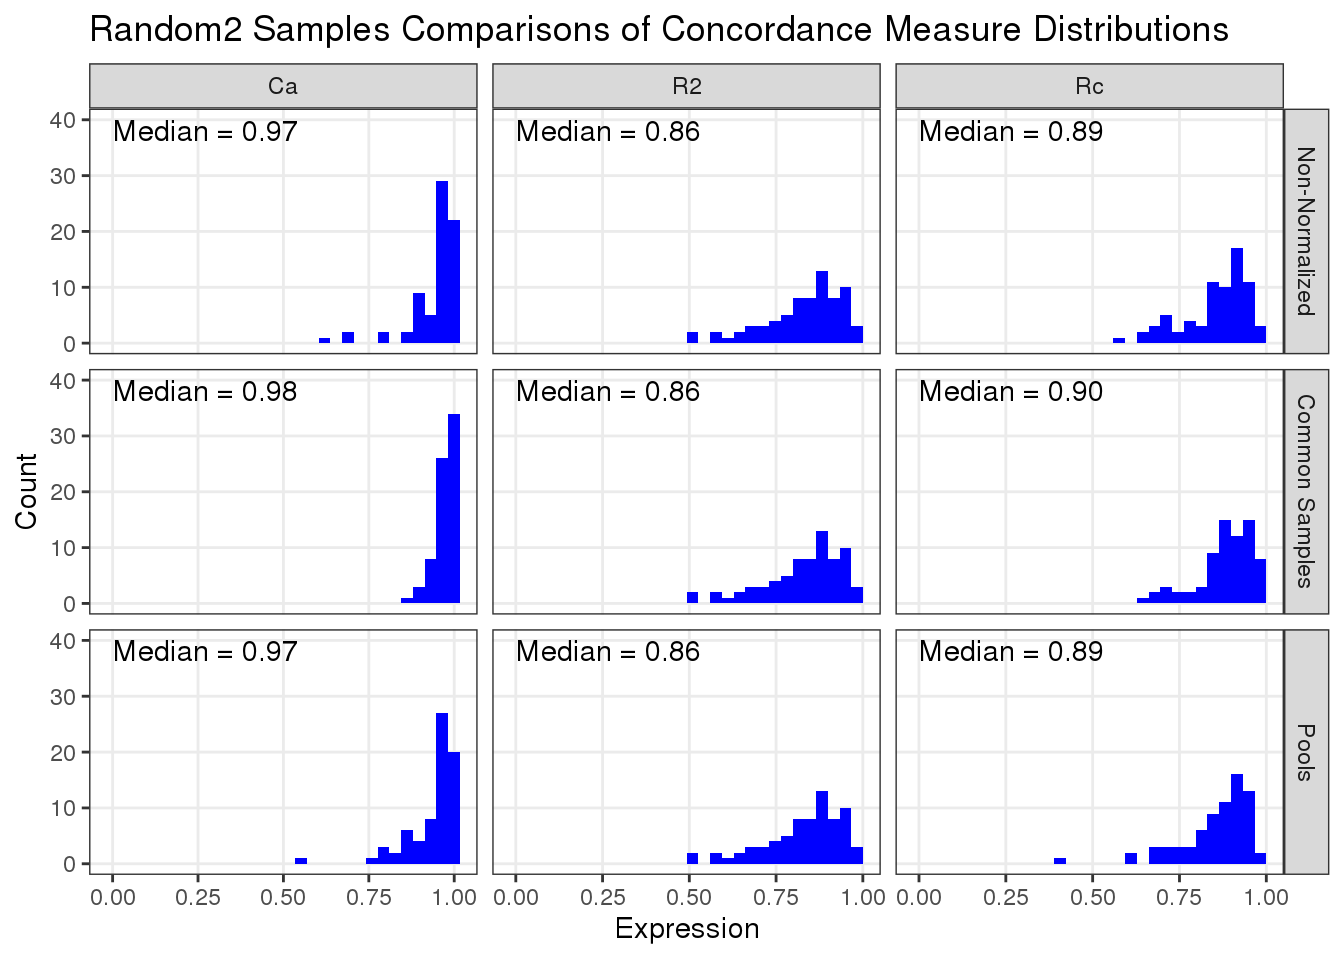
\includegraphics{OV_Histotypes_RSF_files/figure-latex/rand2-vs-pools-1} 

}

\caption{Random2 Samples Comparisons of Concordance Measure Distributions}\label{fig:rand2-vs-pools}
\end{figure}

\begin{table}

\caption{\label{tab:rand2-vs-pools-stats}Random2 Samples Comparisons Statistics by Histotypes}
\centering
\begin{tabular}[t]{l|r|r|r|r|r|r|r|r|r}
\hline
hist & R2-Non & Ca-Non & Rc-Non & R2-Common & Ca-Common & Rc-Common & R2-Pools & Ca-Pools & Rc-Pools\\
\hline
CCOC & NA & NA & NA & NA & NA & NA & NA & NA & NA\\
\hline
ENOC & NA & NA & NA & NA & NA & NA & NA & NA & NA\\
\hline
HGSC & 0.84 & 0.96 & 0.87 & 0.84 & 0.98 & 0.89 & 0.84 & 0.96 & 0.86\\
\hline
LGSC & 1.00 & 0.88 & 0.87 & 1.00 & 0.88 & 0.88 & 1.00 & 0.85 & 0.85\\
\hline
MUC & 0.97 & 0.95 & 0.91 & 0.97 & 0.94 & 0.90 & 0.97 & 0.96 & 0.92\\
\hline
\end{tabular}
\end{table}

\begin{figure}[H]

{\centering 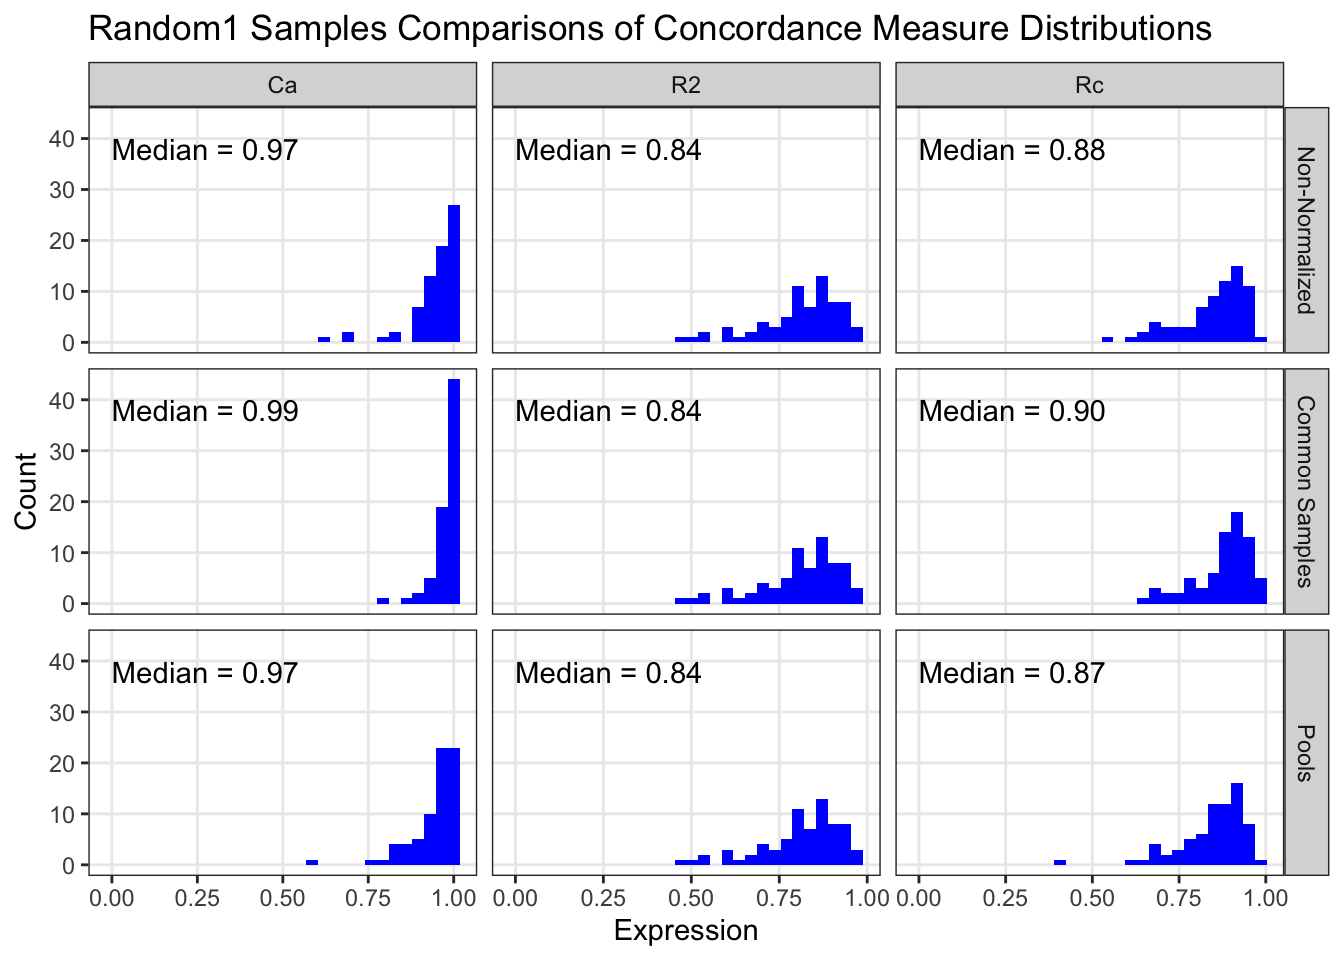
\includegraphics{OV_Histotypes_RSF_files/figure-latex/rand1-vs-pools-1} 

}

\caption{Random1 Samples Comparisons of Concordance Measure Distributions}\label{fig:rand1-vs-pools}
\end{figure}

\begin{table}

\caption{\label{tab:rand1-vs-pools-stats}Random1 Samples Comparisons Statistics by Histotypes}
\centering
\begin{tabular}[t]{l|r|r|r|r|r|r|r|r|r}
\hline
hist & R2-Non & Ca-Non & Rc-Non & R2-Common & Ca-Common & Rc-Common & R2-Pools & Ca-Pools & Rc-Pools\\
\hline
CCOC & 1.00 & 0.23 & 0.08 & 1.00 & 0.27 & 0.16 & 1.00 & 0.15 & 0.09\\
\hline
ENOC & 1.00 & 0.63 & 0.61 & 1.00 & 0.61 & 0.57 & 1.00 & 0.61 & 0.61\\
\hline
HGSC & 0.83 & 0.96 & 0.86 & 0.83 & 0.98 & 0.89 & 0.83 & 0.96 & 0.86\\
\hline
LGSC & 0.98 & 0.92 & 0.90 & 0.98 & 0.95 & 0.93 & 0.98 & 0.92 & 0.90\\
\hline
MUC & 0.68 & 0.77 & 0.55 & 0.68 & 0.86 & 0.61 & 0.68 & 0.78 & 0.51\\
\hline
\end{tabular}
\end{table}

\begin{table}

\caption{\label{tab:cs23-dsc}DSC for CS2 vs CS3 Comparisons}
\centering
\begin{tabular}[t]{l|r|r}
\hline
Comparison & DSC & pval\\
\hline
CS2-None vs CS3 & 0.126 & 0.032\\
\hline
CS2-Random1 vs CS3 & 0.084 & 0.475\\
\hline
CS2-Pools vs CS3 & 0.159 & 0.005\\
\hline
\end{tabular}
\end{table}

\hypertarget{codeset-chaining}{%
\subsection{CodeSet Chaining}\label{codeset-chaining}}

\hypertarget{cs1-cs2-cs3}{%
\subsubsection{CS1, CS2, CS3}\label{cs1-cs2-cs3}}

\begin{figure}[H]

{\centering 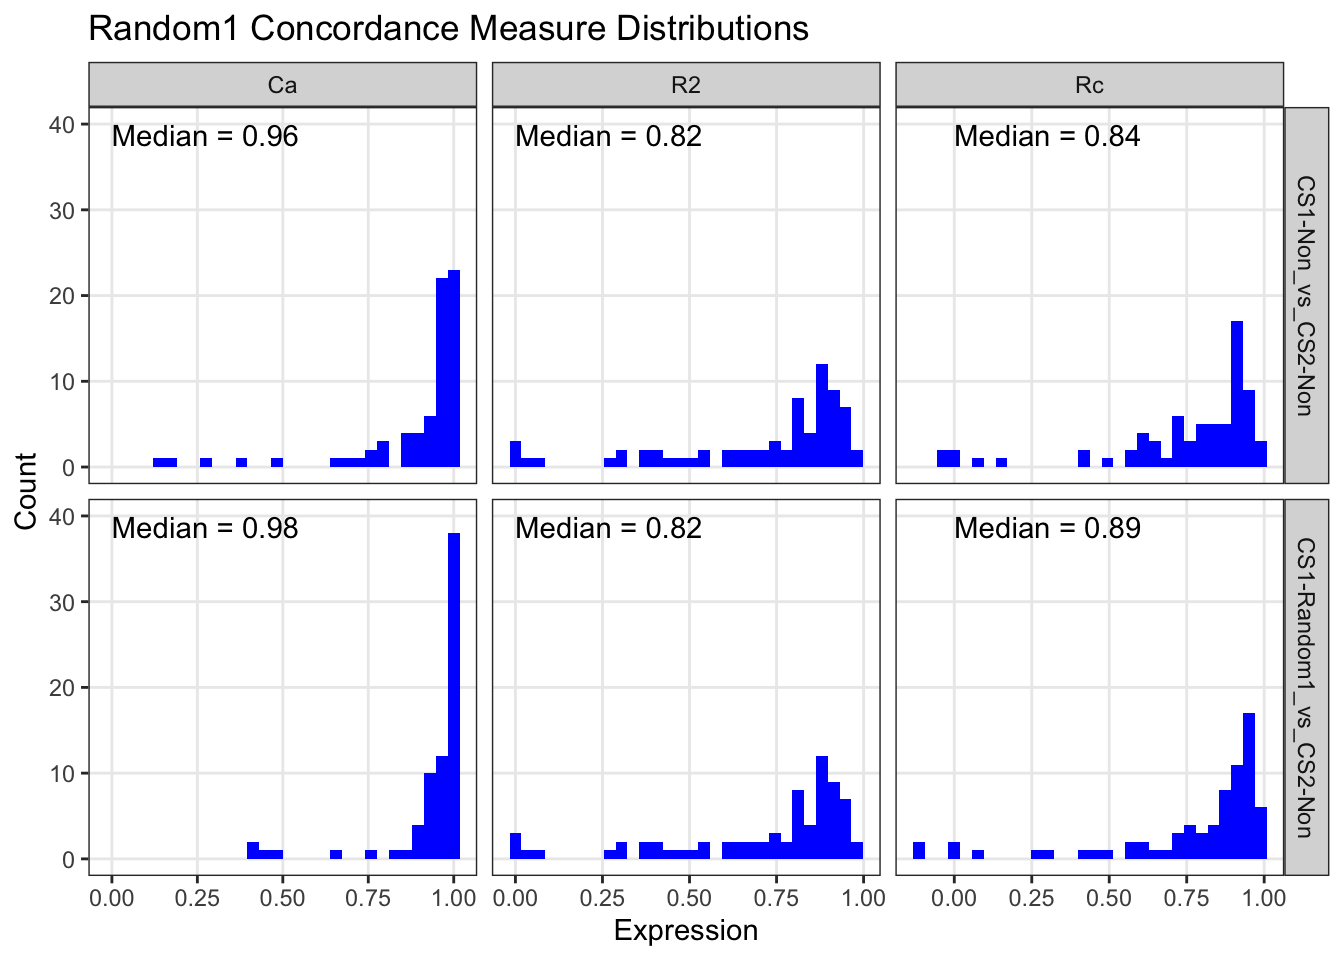
\includegraphics{OV_Histotypes_RSF_files/figure-latex/cs-chain-rand1-1} 

}

\caption{Random1 Concordance Measure Distributions}\label{fig:cs-chain-rand1}
\end{figure}

\begin{figure}[H]

{\centering 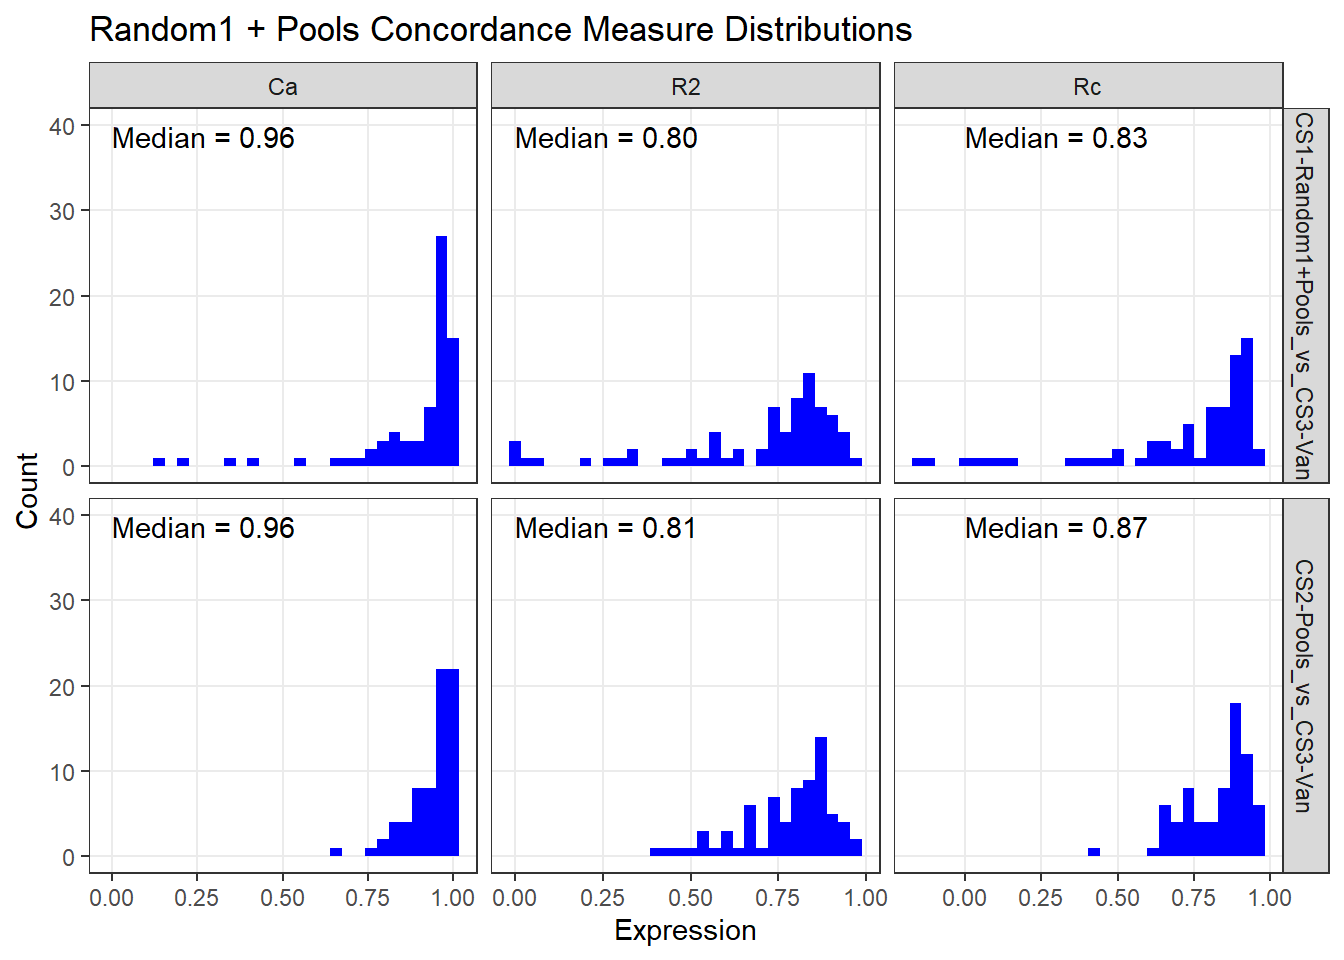
\includegraphics{OV_Histotypes_RSF_files/figure-latex/cs-chain-rand1-cs2pools-1} 

}

\caption{Random1 + Pools Concordance Measure Distributions}\label{fig:cs-chain-rand1-cs2pools}
\end{figure}

\begin{figure}[H]

{\centering 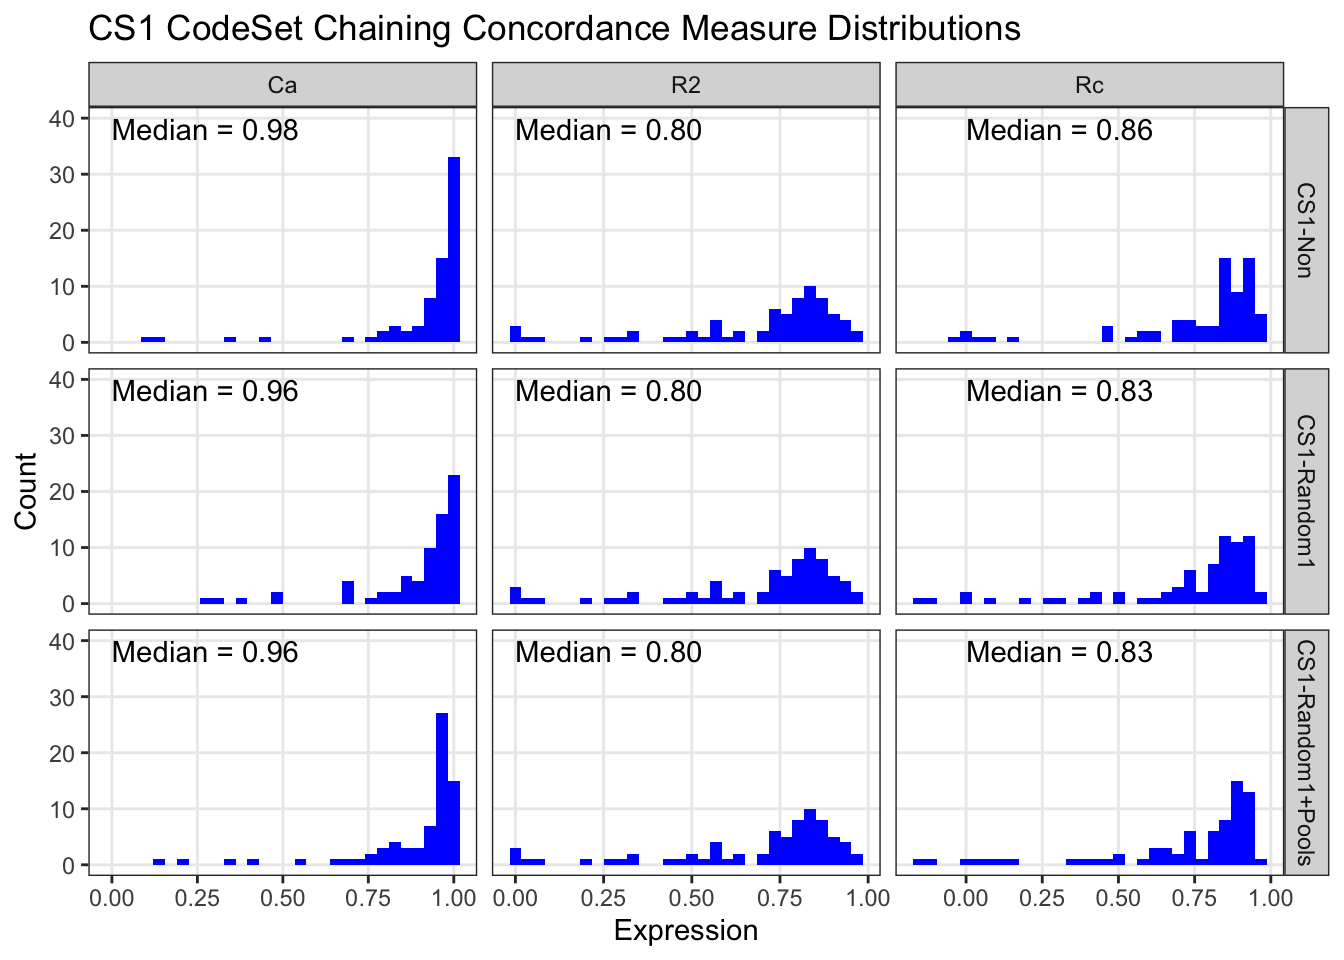
\includegraphics{OV_Histotypes_RSF_files/figure-latex/cs-chain-rand1-cs1v3-1} 

}

\caption{CS1 CodeSet Chaining Concordance Measure Distributions}\label{fig:cs-chain-rand1-cs1v3}
\end{figure}

\begin{figure}[H]

{\centering 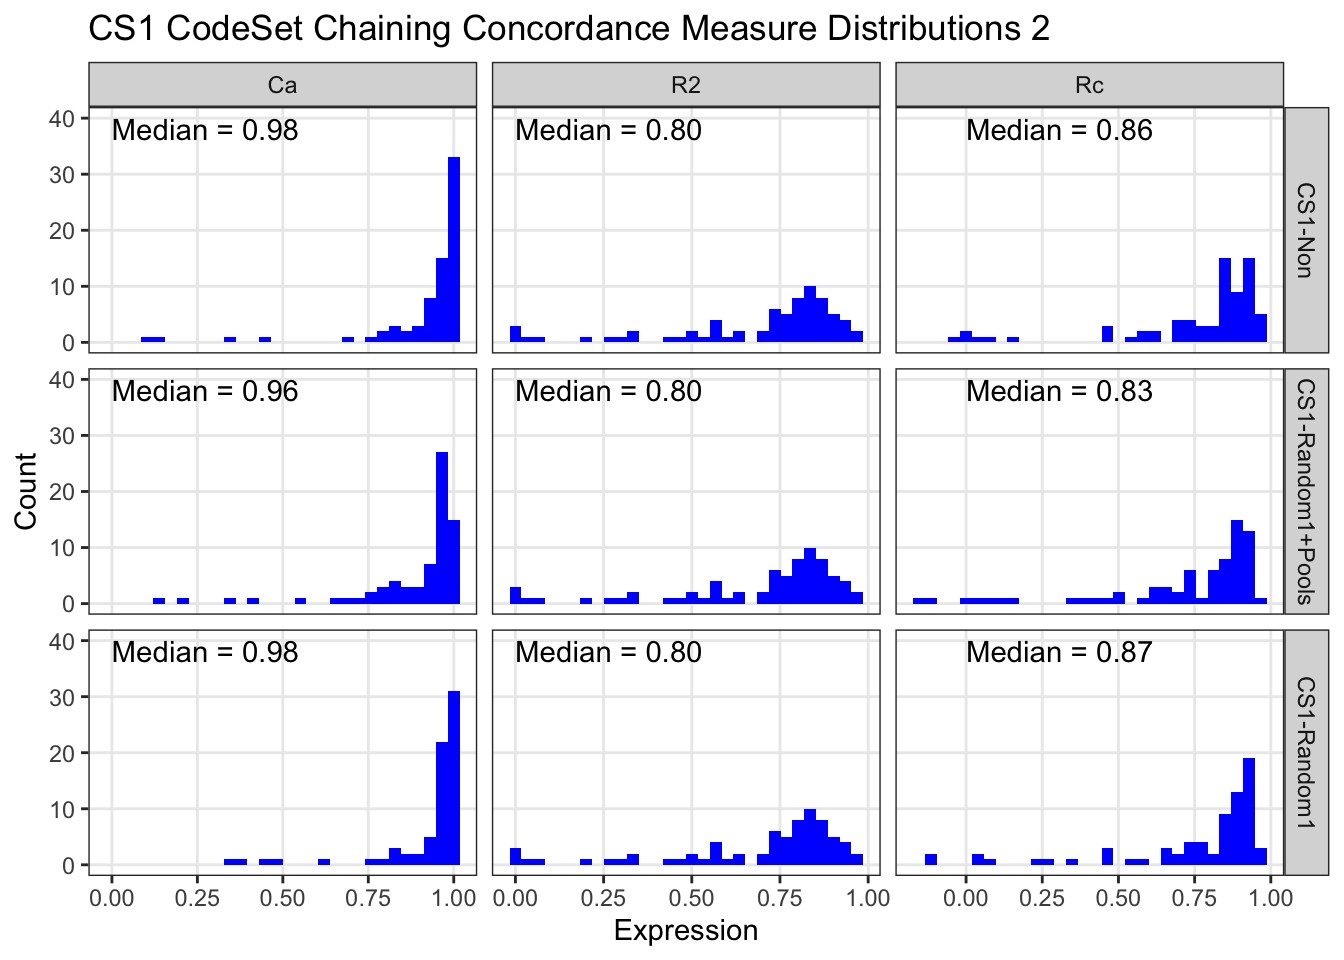
\includegraphics{OV_Histotypes_RSF_files/figure-latex/cs-chain-rand1-cs1v3-2-1} 

}

\caption{CS1 CodeSet Chaining Concordance Measure Distributions 2}\label{fig:cs-chain-rand1-cs1v3-2}
\end{figure}

\begin{table}

\caption{\label{tab:cs13-dsc}DSC for CS1 vs CS3 Comparisons}
\centering
\begin{tabular}[t]{l|r|r}
\hline
Comparison & DSC & pval\\
\hline
CS1-None vs CS3 & 0.265 & 0\\
\hline
CS1-Random1+Pools vs CS3 & 0.351 & 0\\
\hline
CS1-Random1 vs CS3 & 0.229 & 0\\
\hline
\end{tabular}
\end{table}

\begin{figure}[H]

{\centering 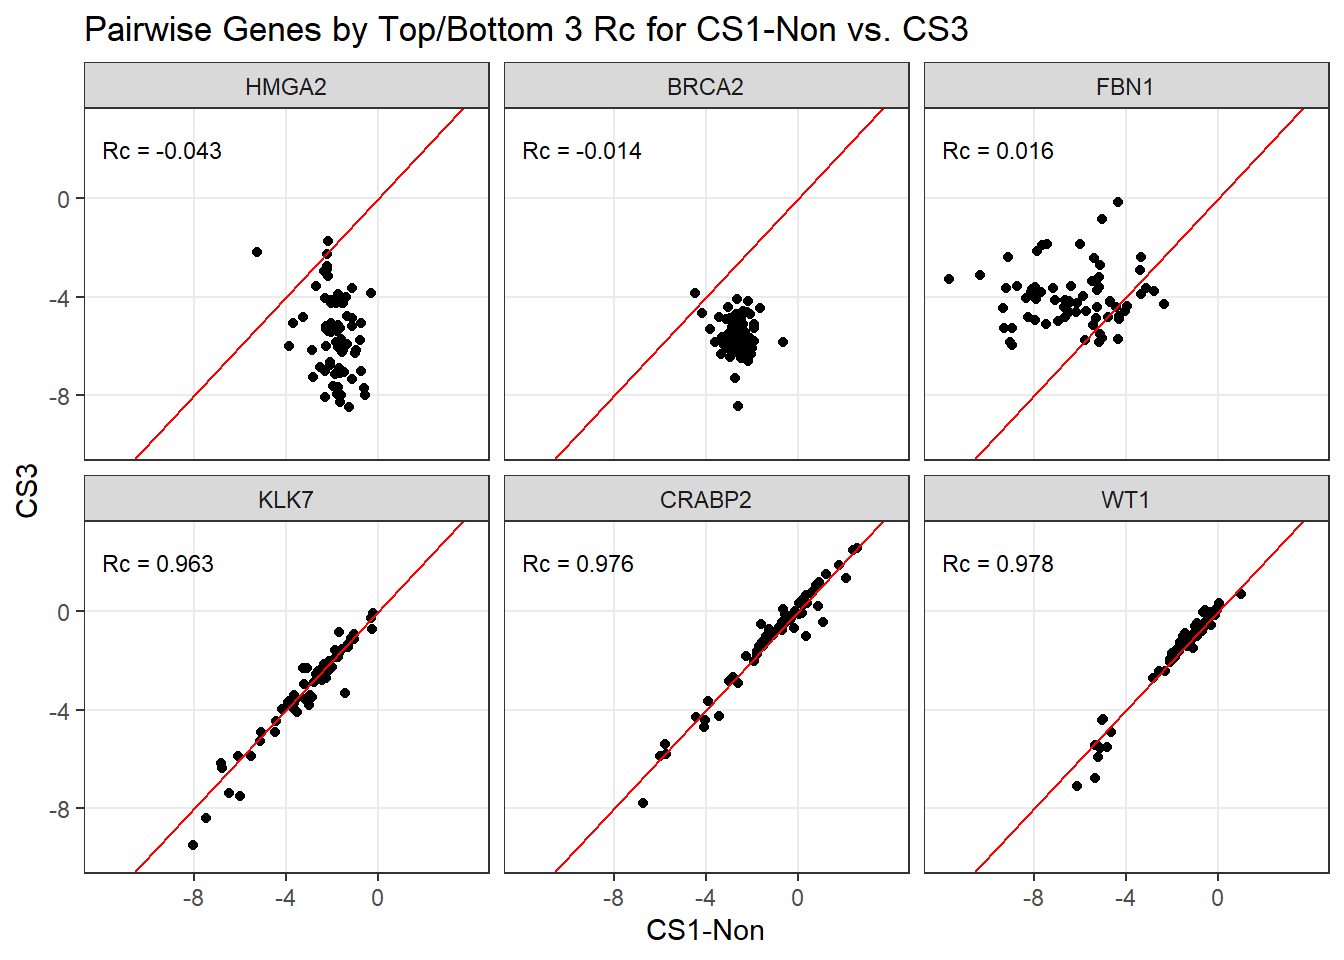
\includegraphics{OV_Histotypes_RSF_files/figure-latex/cs13-genes-topbot-non-1} 

}

\caption{Pairwise Genes by Top/Bottom 3 Rc for CS1-Non vs. CS3}\label{fig:cs13-genes-topbot-non}
\end{figure}

\begin{figure}[H]

{\centering 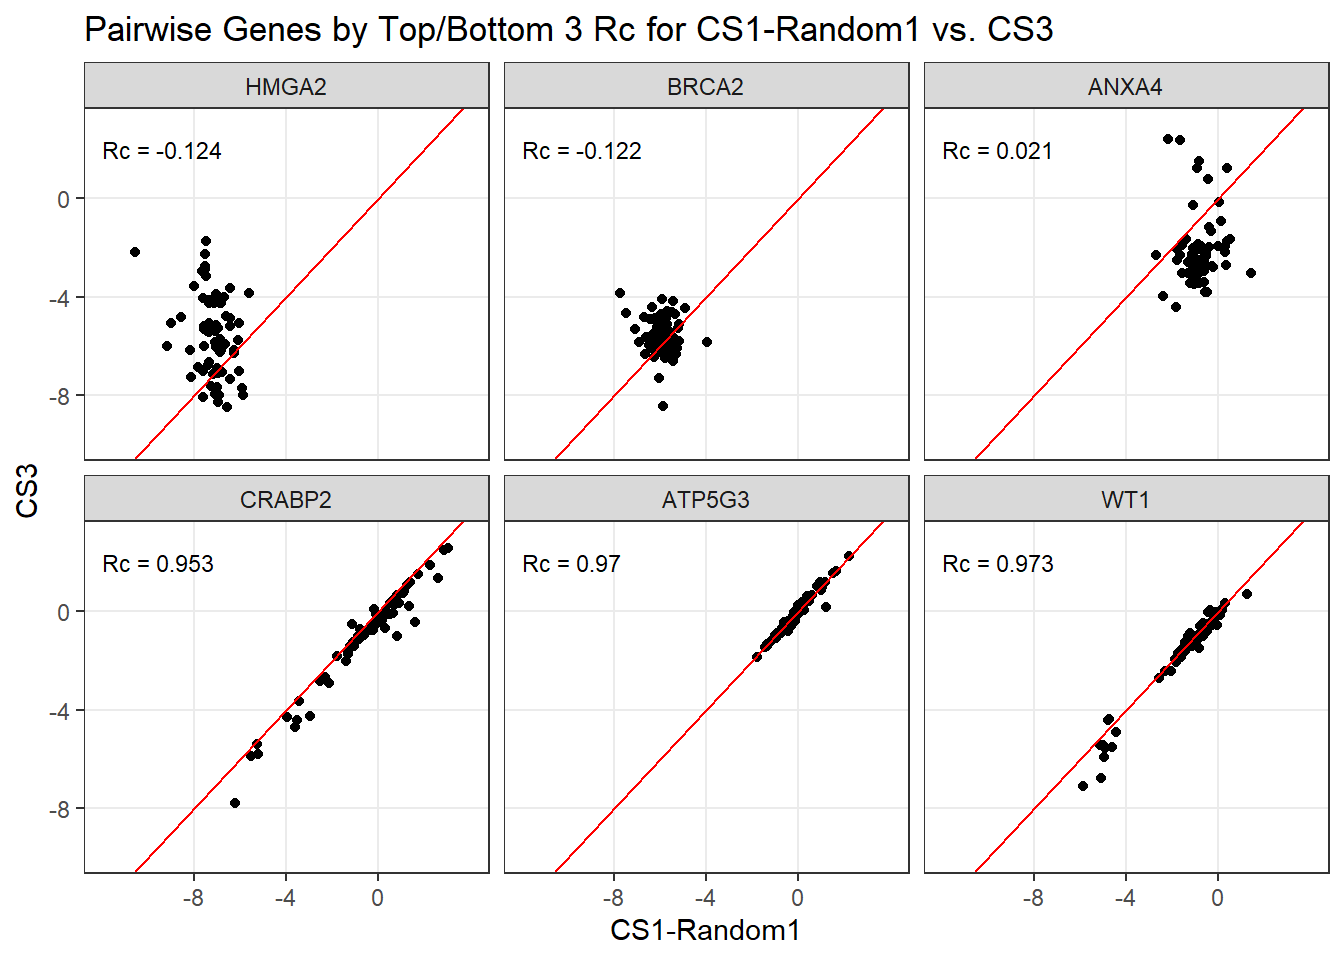
\includegraphics{OV_Histotypes_RSF_files/figure-latex/cs13-genes-topbot-rand1-1} 

}

\caption{Pairwise Genes by Top/Bottom 3 Rc for CS1-Random1 vs. CS3}\label{fig:cs13-genes-topbot-rand1}
\end{figure}

\begin{figure}[H]

{\centering 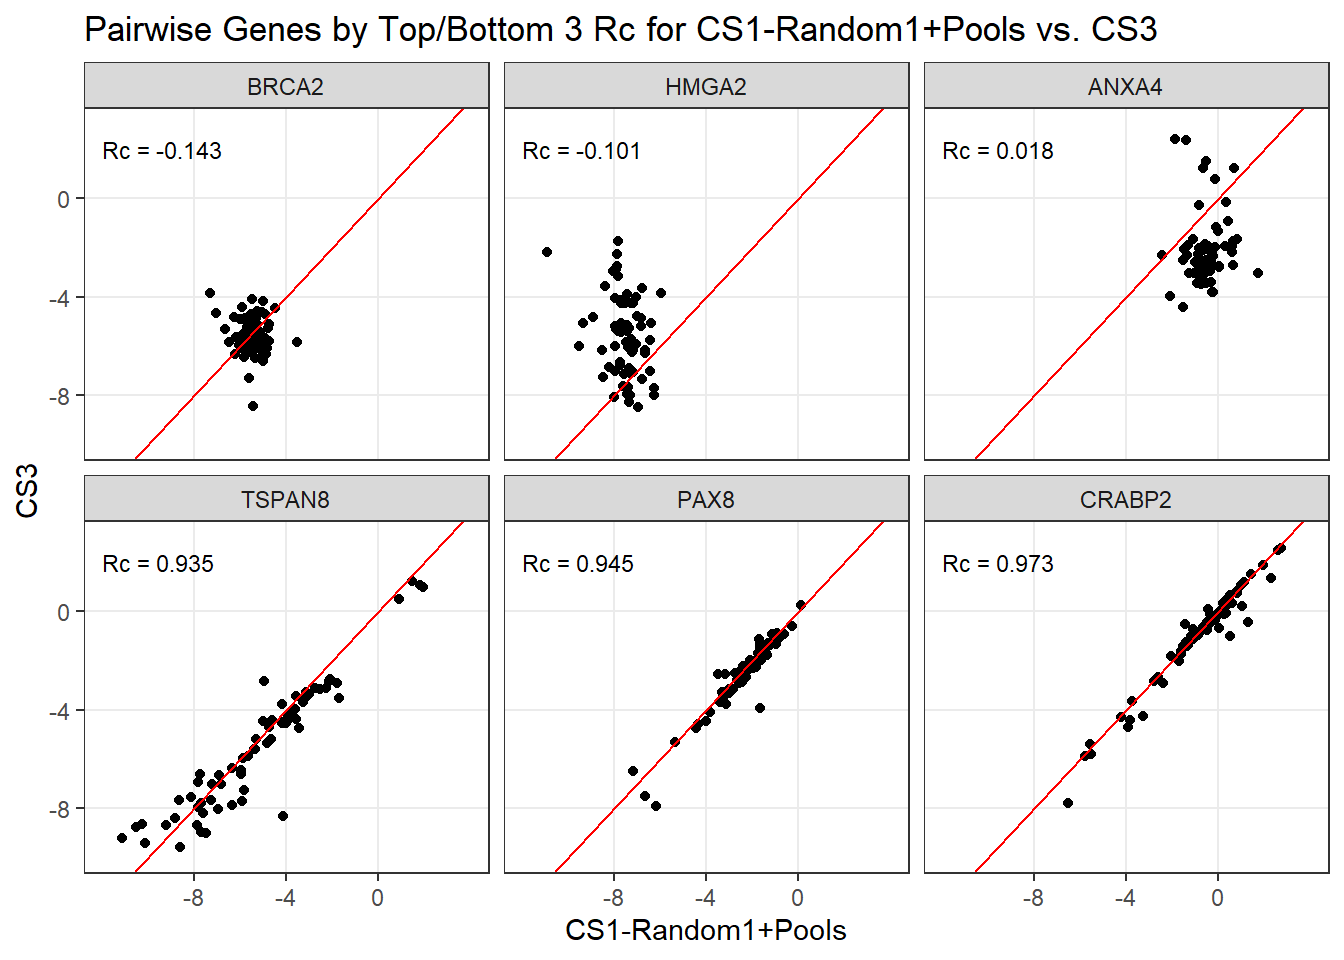
\includegraphics{OV_Histotypes_RSF_files/figure-latex/cs13-genes-topbot-rand1pools-1} 

}

\caption{Pairwise Genes by Top/Bottom 3 Rc for CS1-Random1+Pools vs. CS3}\label{fig:cs13-genes-topbot-rand1pools}
\end{figure}

\begin{figure}[H]

{\centering 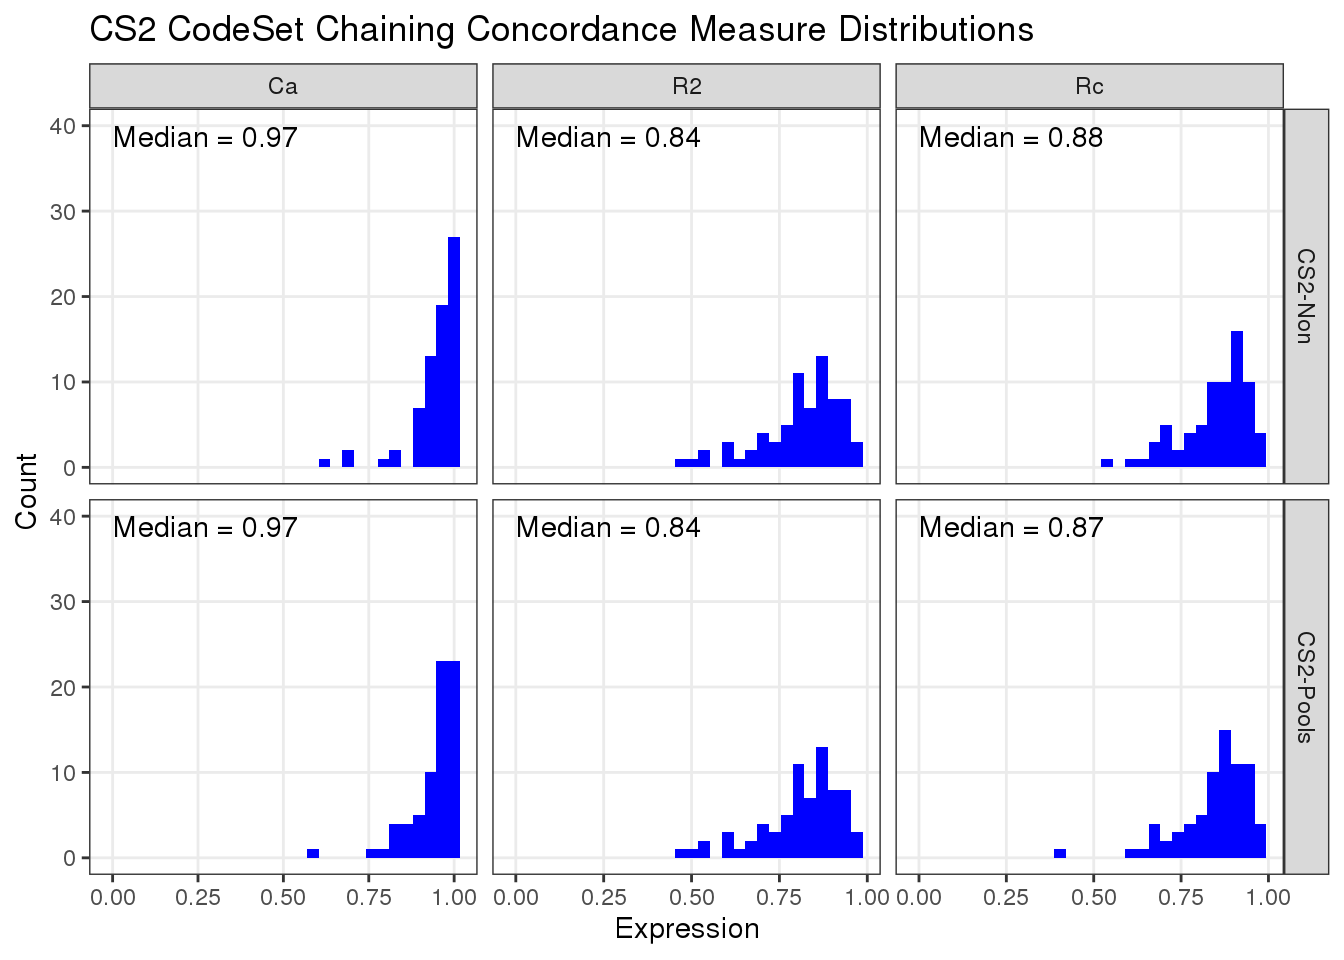
\includegraphics{OV_Histotypes_RSF_files/figure-latex/cs-chain-rand1-cs2v3-1} 

}

\caption{CS2 CodeSet Chaining Concordance Measure Distributions}\label{fig:cs-chain-rand1-cs2v3}
\end{figure}

\hypertarget{cs3-cs4-cs5-using-set-ba}{%
\subsubsection{CS3, CS4, CS5 using Set B/A}\label{cs3-cs4-cs5-using-set-ba}}

\begin{figure}[H]

{\centering 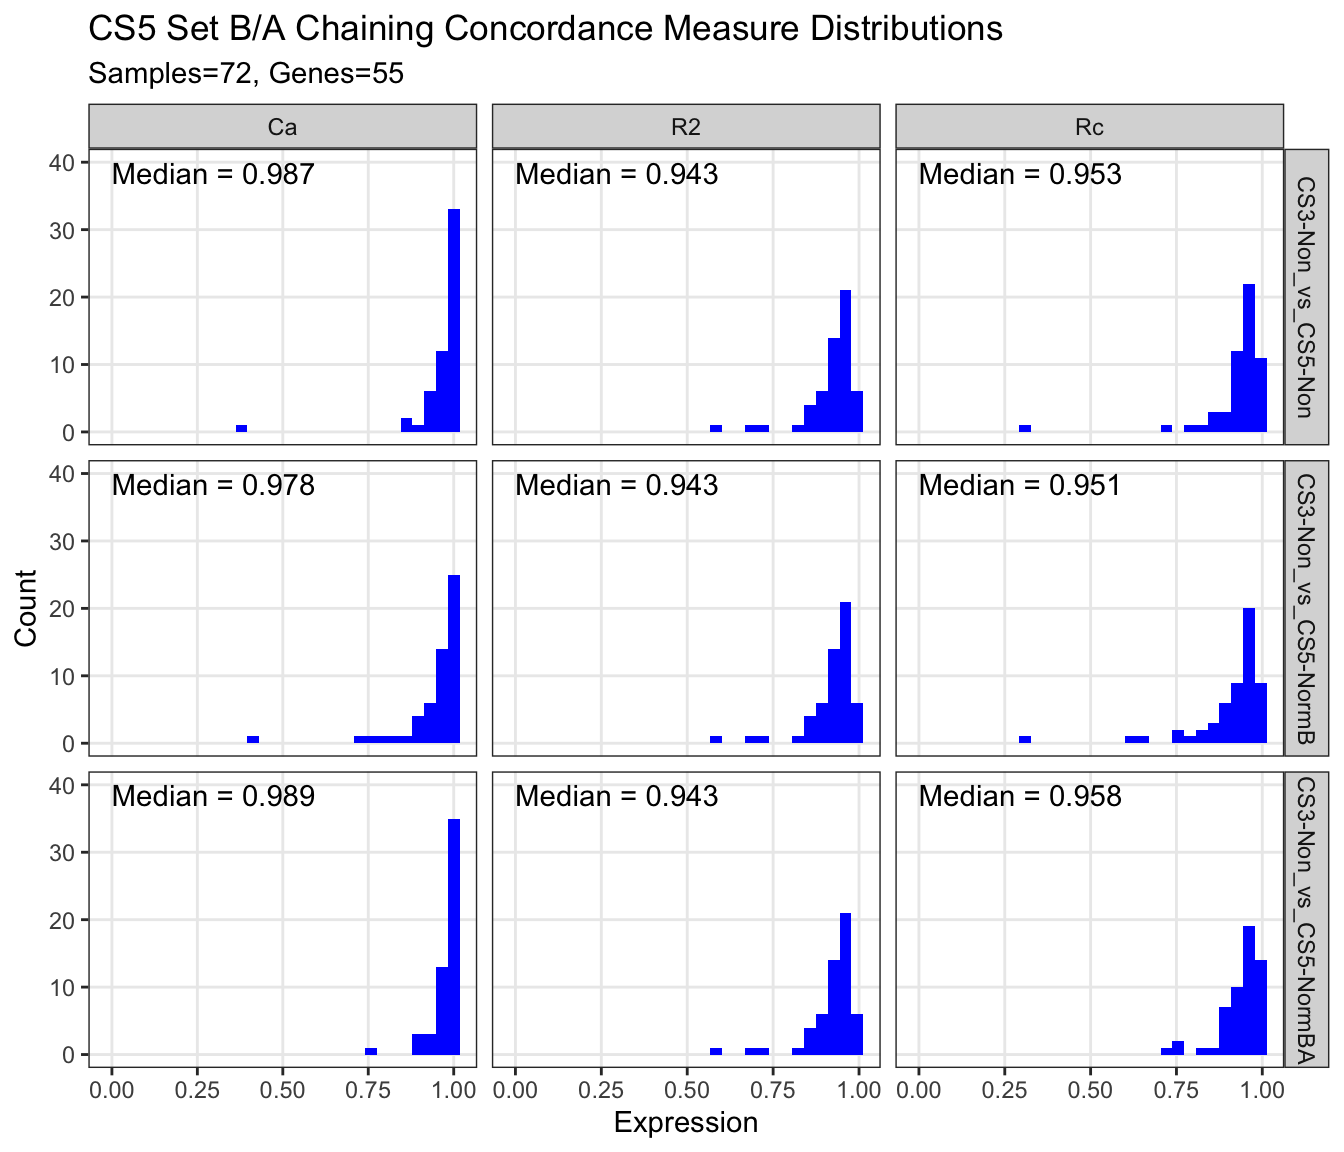
\includegraphics{OV_Histotypes_RSF_files/figure-latex/cs-chain-cs5-setBA-1} 

}

\caption{CS5 Set B/A Chaining Concordance  Measure Distributions}\label{fig:cs-chain-cs5-setBA}
\end{figure}

\begin{figure}[H]

{\centering 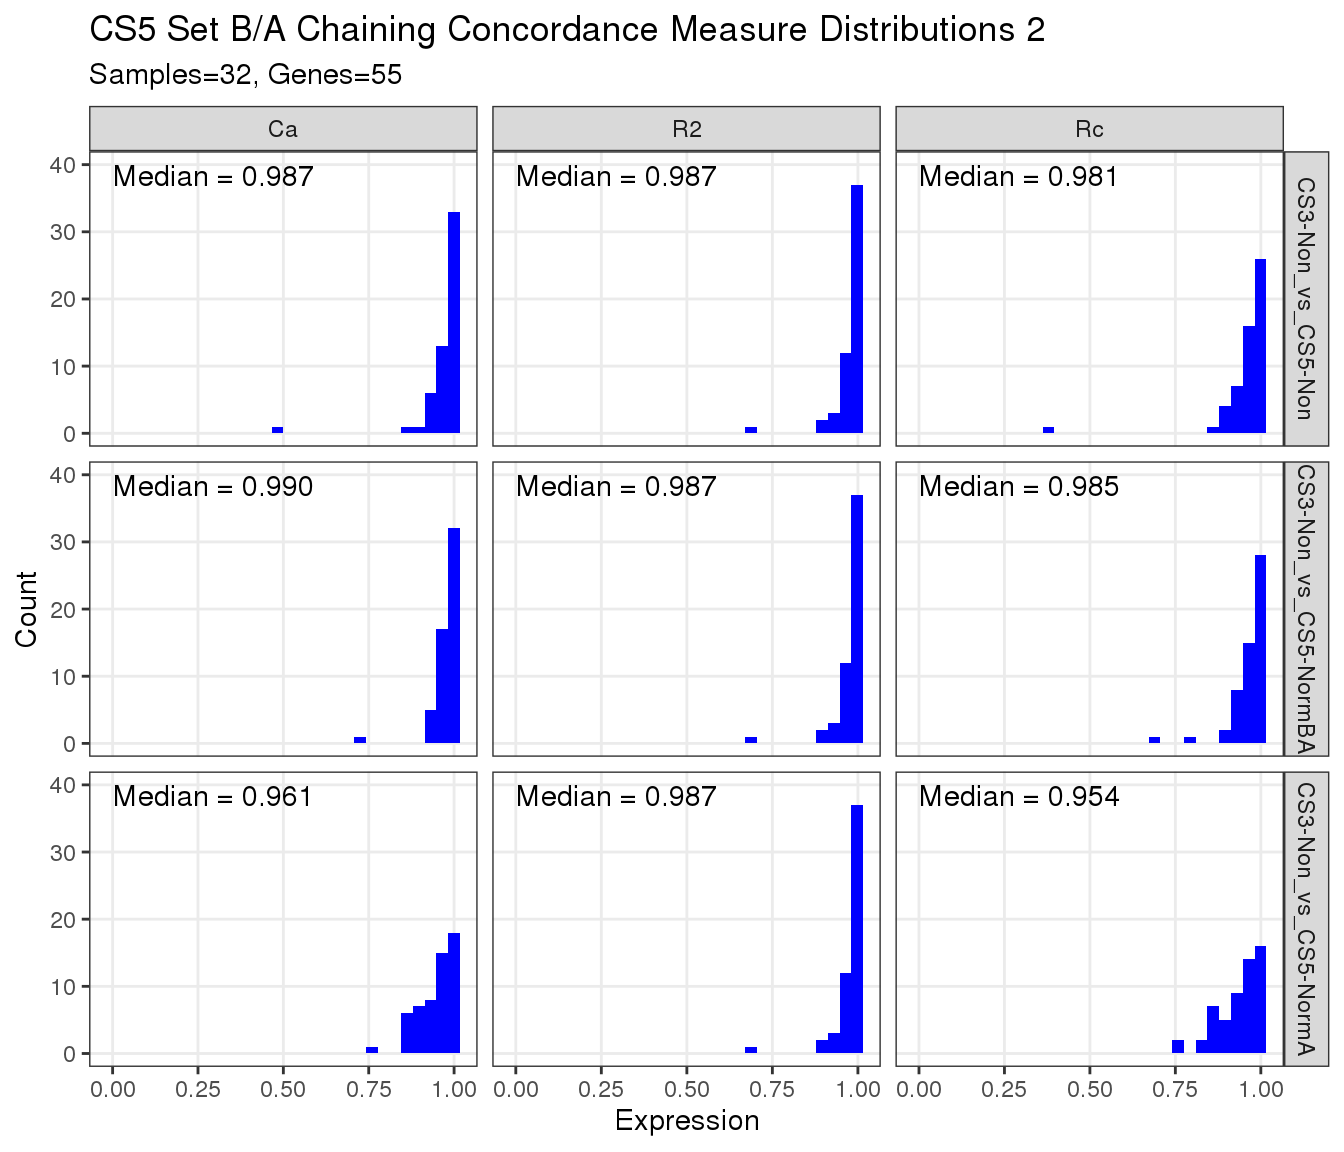
\includegraphics{OV_Histotypes_RSF_files/figure-latex/cs-chain-cs5-setBA-2-1} 

}

\caption{CS5 Set B/A Chaining Concordance  Measure Distributions 2}\label{fig:cs-chain-cs5-setBA-2}
\end{figure}

\begin{table}

\caption{\label{tab:cs35-BA-dsc}DSC for CS3 vs CS5 Set B/A Comparisons}
\centering
\begin{tabular}[t]{l|r|r}
\hline
Comparisons & DSC & pval\\
\hline
CS3 vs CS5-None & 0.126 & 0.101\\
\hline
CS3 vs CS5-NormBA & 0.087 & 0.320\\
\hline
CS3 vs CS5-NormA & 0.144 & 0.047\\
\hline
\end{tabular}
\end{table}

\begin{figure}[H]

{\centering 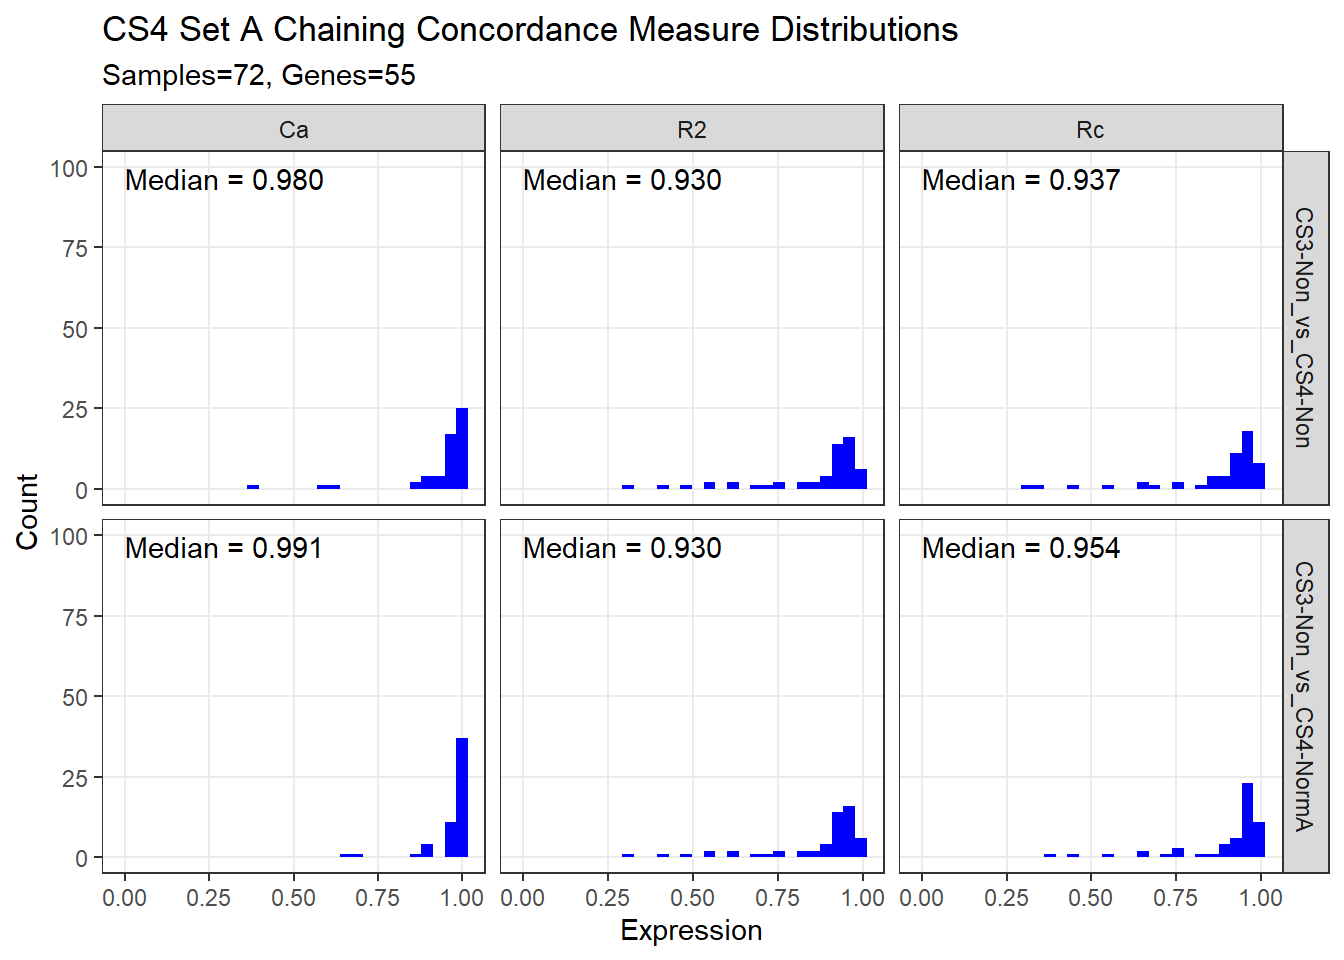
\includegraphics{OV_Histotypes_RSF_files/figure-latex/cs-chain-cs4-setA-1} 

}

\caption{CS4 Set A Chaining Concordance Measure Distributions}\label{fig:cs-chain-cs4-setA}
\end{figure}

\begin{figure}[H]

{\centering 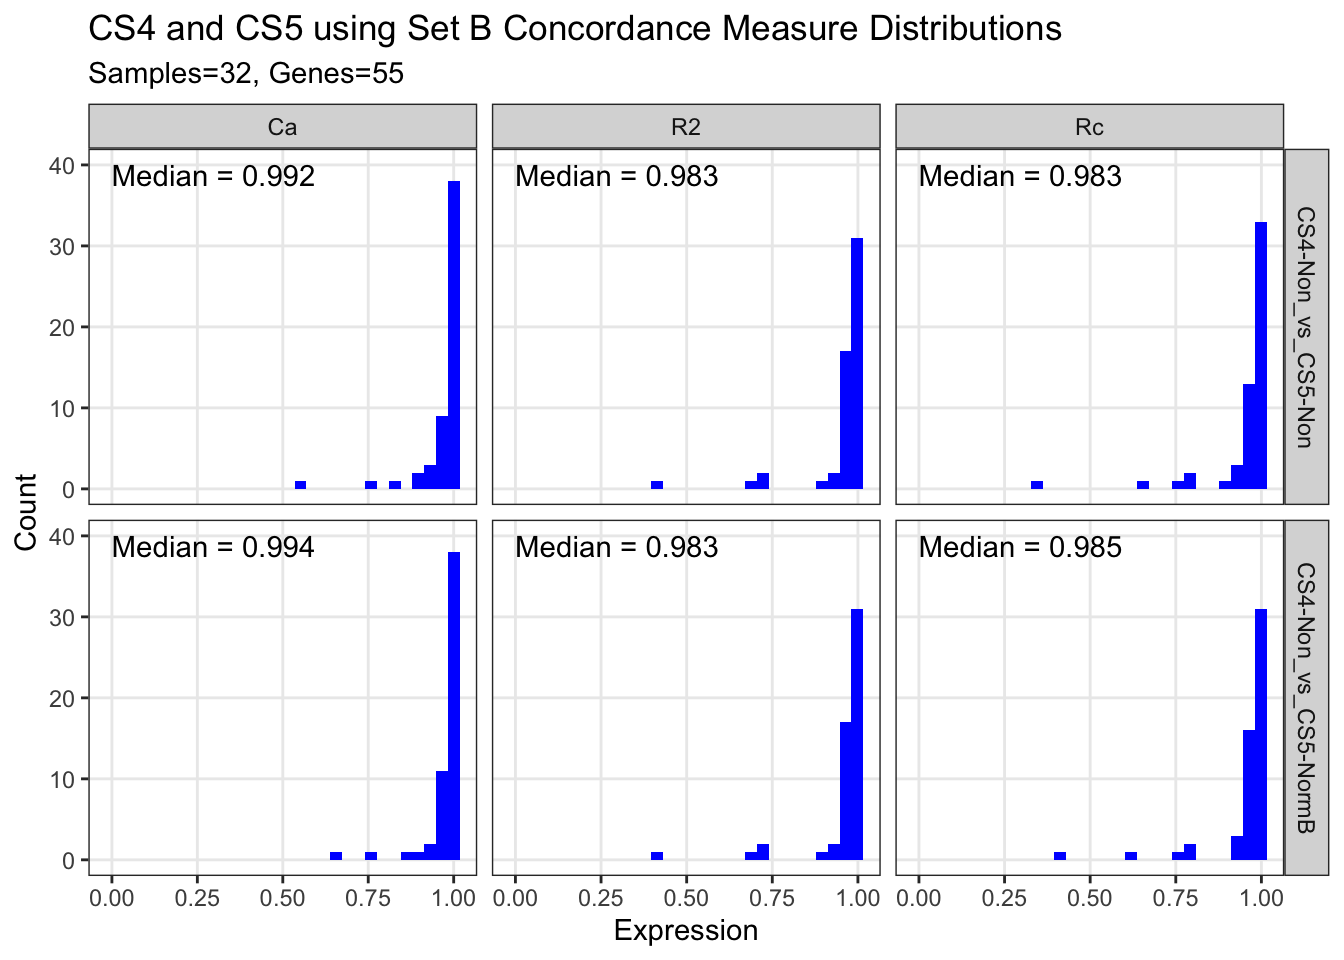
\includegraphics{OV_Histotypes_RSF_files/figure-latex/cs-chain-cs5-cs4-B-1} 

}

\caption{CS4 and CS5 using Set B Concordance Measure Distributions}\label{fig:cs-chain-cs5-cs4-B}
\end{figure}

\hypertarget{cs3-cs4-cs5-using-set-ca}{%
\subsubsection{CS3, CS4, CS5 using Set C/A}\label{cs3-cs4-cs5-using-set-ca}}

\begin{figure}[H]

{\centering 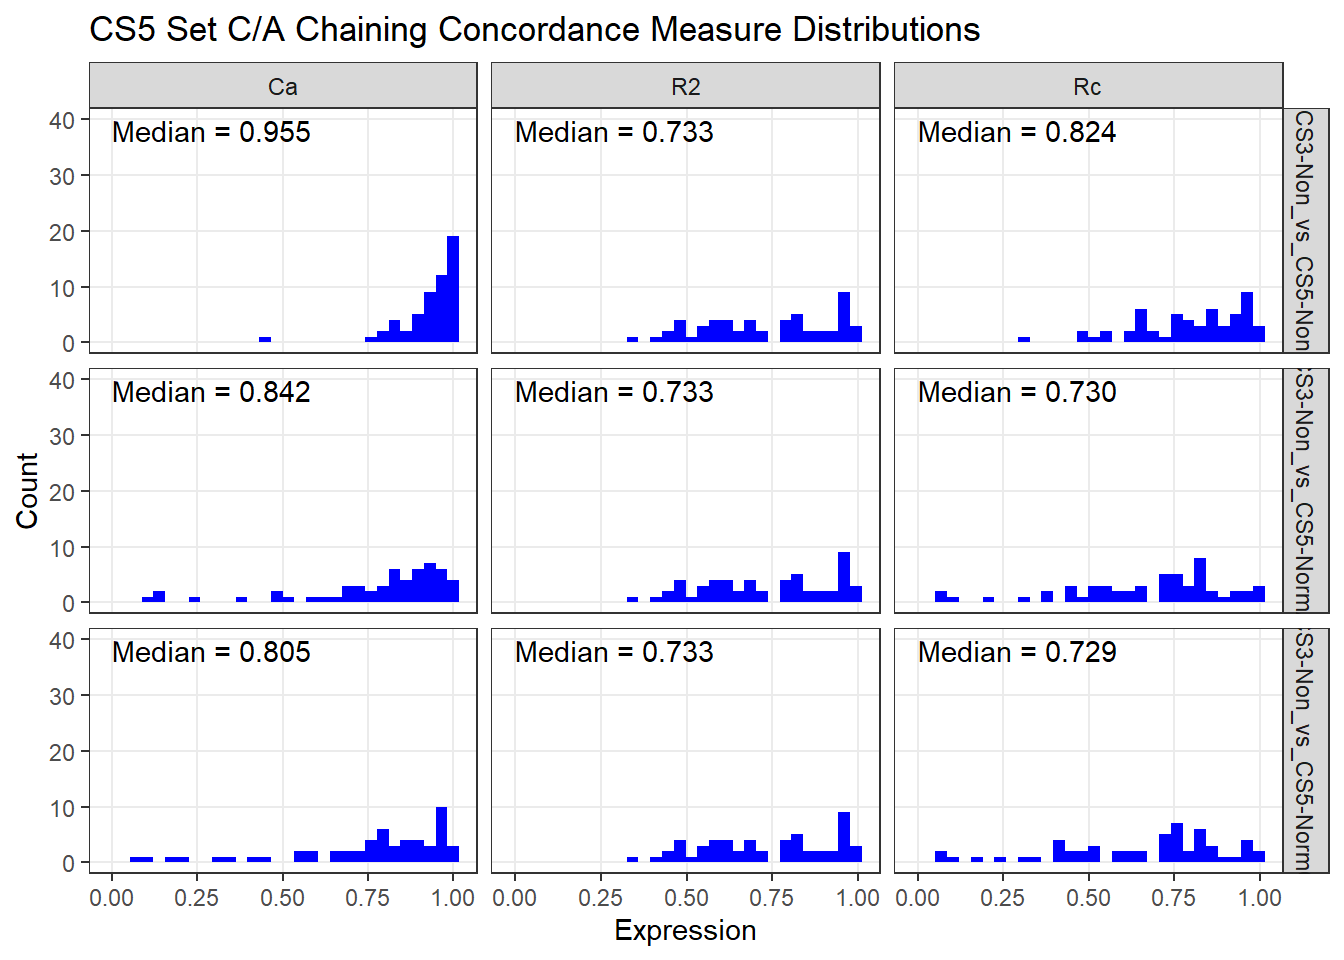
\includegraphics{OV_Histotypes_RSF_files/figure-latex/cs-chain-cs5-setCA-1} 

}

\caption{CS5 Set C/A Chaining Concordance  Measure Distributions}\label{fig:cs-chain-cs5-setCA}
\end{figure}

\begin{figure}[H]

{\centering 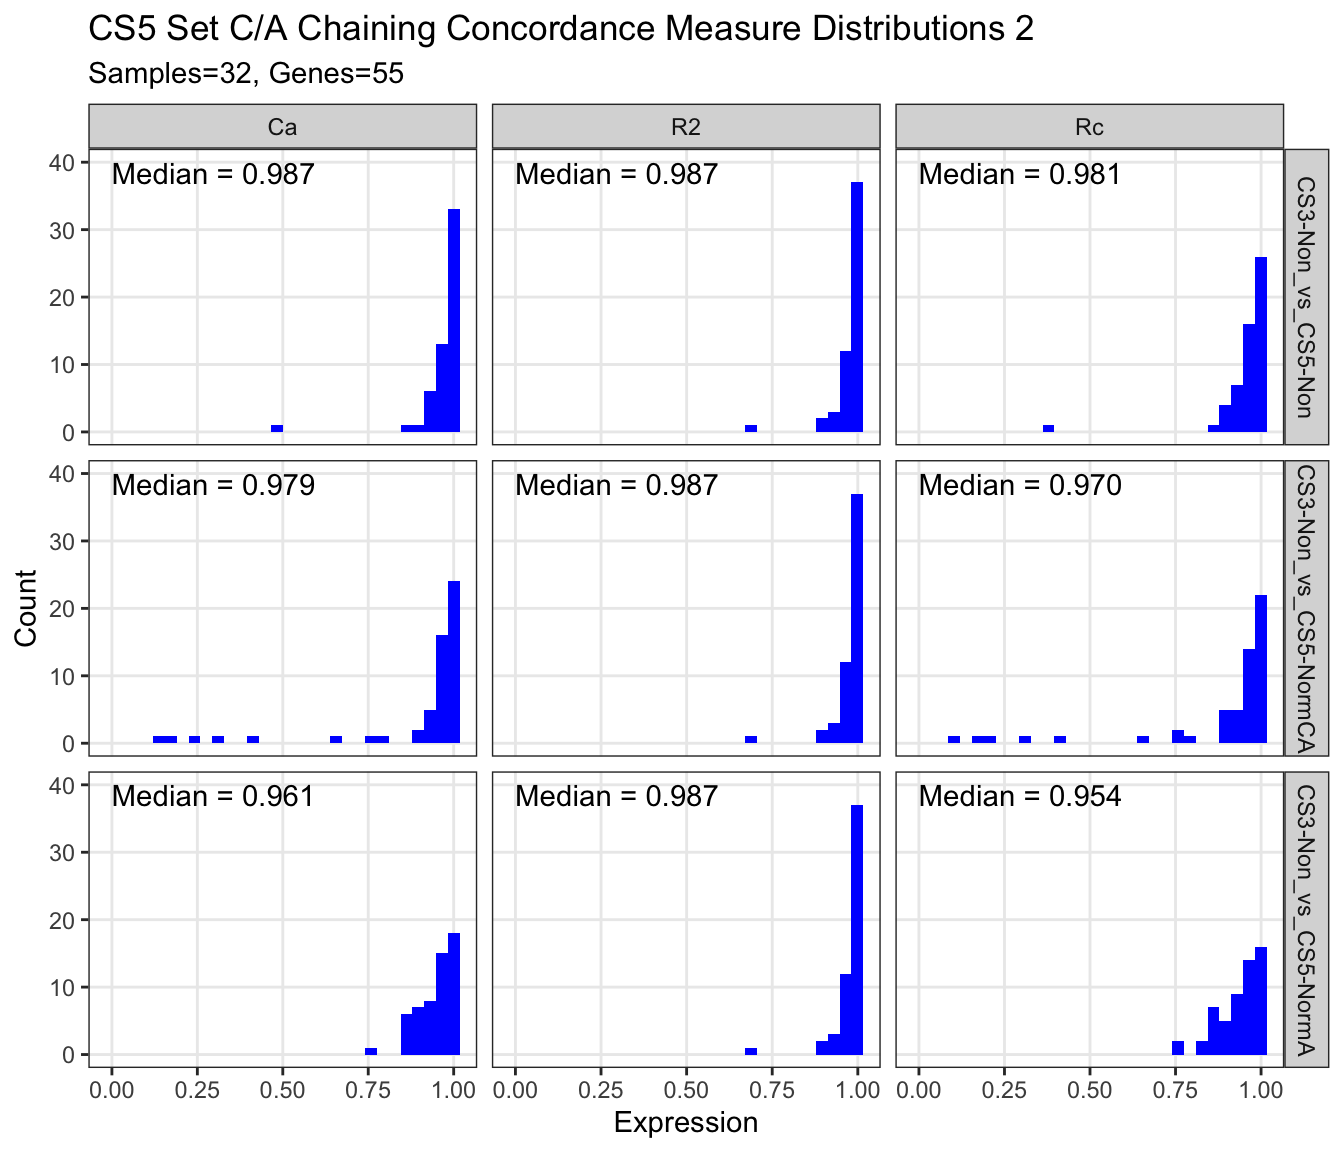
\includegraphics{OV_Histotypes_RSF_files/figure-latex/cs-chain-cs5-setCA-2-1} 

}

\caption{CS5 Set C/A Chaining Concordance  Measure Distributions 2}\label{fig:cs-chain-cs5-setCA-2}
\end{figure}

\begin{table}

\caption{\label{tab:cs35-CA-dsc}DSC for CS3 vs CS5 Set C/A Comparisons}
\centering
\begin{tabular}[t]{l|r|r}
\hline
Comparisons & DSC & pval\\
\hline
CS3 vs CS5-None & 0.126 & 0.101\\
\hline
CS3 vs CS5-NormCA & 0.383 & 0.000\\
\hline
CS3 vs CS5-NormA & 0.144 & 0.047\\
\hline
\end{tabular}
\end{table}

\begin{figure}[H]

{\centering 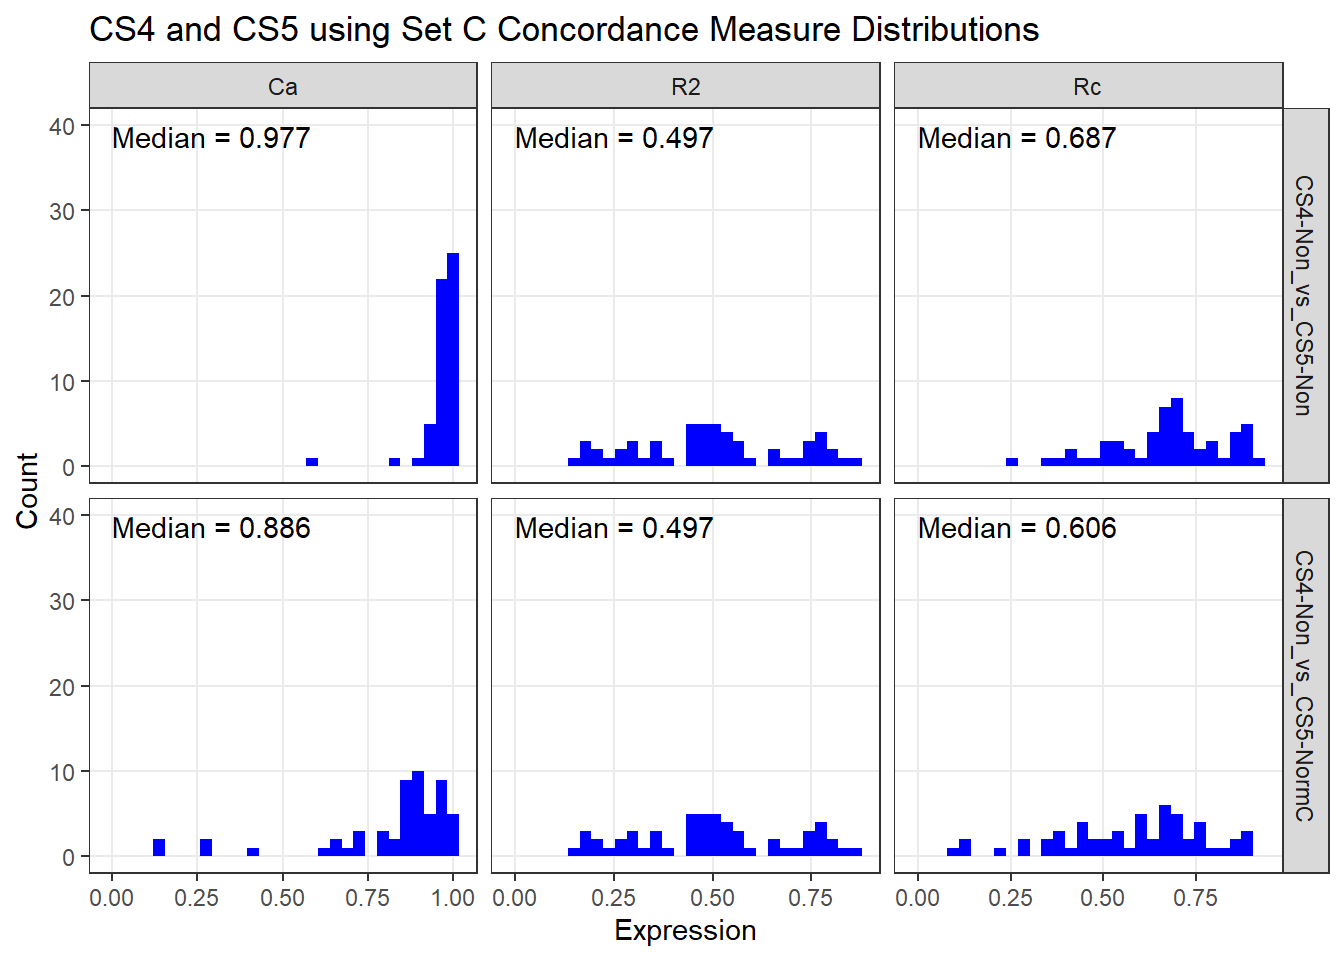
\includegraphics{OV_Histotypes_RSF_files/figure-latex/cs-chain-cs5-cs4-C-1} 

}

\caption{CS4 and CS5 using Set C Concordance Measure Distributions}\label{fig:cs-chain-cs5-cs4-C}
\end{figure}

\hypertarget{common-sample-distributions}{%
\section{Common Sample Distributions}\label{common-sample-distributions}}

\begin{table}

\caption{\label{tab:common-dist-all}All Common Samples Histotype Distribution}
\centering
\begin{tabular}[t]{l|r|r|r}
\hline
revHist & CS1 & CS2 & CS3\\
\hline
CCOC & 3 & 4 & 3\\
\hline
ENOC & 4 & 4 & 3\\
\hline
HGSC & 59 & 62 & 75\\
\hline
LGSC & 7 & 5 & 4\\
\hline
MUC & 7 & 5 & 5\\
\hline
\end{tabular}
\end{table}

\begin{table}

\caption{\label{tab:common-dist-distinct}Distinct Common Samples Histotype Distribution}
\centering
\begin{tabular}[t]{l|r|r|r}
\hline
revHist & CS1 & CS2 & CS3\\
\hline
CCOC & 3 & 3 & 3\\
\hline
ENOC & 3 & 3 & 3\\
\hline
HGSC & 57 & 57 & 57\\
\hline
LGSC & 4 & 4 & 4\\
\hline
MUC & 5 & 5 & 5\\
\hline
\end{tabular}
\end{table}

\begin{table}

\caption{\label{tab:common-cs2-cs3-dist-distinct}Distinct Common CS2 and CS3 Samples Histotype Distribution}
\centering
\begin{tabular}[t]{l|r|r}
\hline
revHist & CS2 & CS3\\
\hline
CCOC & 3 & 3\\
\hline
ENOC & 3 & 3\\
\hline
HGSC & 71 & 71\\
\hline
LGSC & 4 & 4\\
\hline
MUC & 5 & 5\\
\hline
\end{tabular}
\end{table}

\begin{table}

\caption{\label{tab:common-dist-sites}Common Samples Across Sites Histotype Distribution}
\centering
\begin{tabular}[t]{l|r|r|r}
\hline
revHist & AOC & USC & Vancouver\\
\hline
CCOC & 3 & 3 & 3\\
\hline
ENOC & 3 & 3 & 3\\
\hline
HGSC & 13 & 13 & 27\\
\hline
LGSC & 2 & 2 & 2\\
\hline
MUC & 3 & 3 & 3\\
\hline
\end{tabular}
\end{table}

\begin{table}

\caption{\label{tab:common-dist-sites-distinct}Distinct Common Samples Across Sites Histotype Distribution}
\centering
\begin{tabular}[t]{l|r|r|r}
\hline
revHist & AOC & USC & Vancouver\\
\hline
CCOC & 3 & 3 & 3\\
\hline
ENOC & 3 & 3 & 3\\
\hline
HGSC & 13 & 13 & 13\\
\hline
LGSC & 2 & 2 & 2\\
\hline
MUC & 3 & 3 & 3\\
\hline
\end{tabular}
\end{table}

\begin{table}

\caption{\label{tab:cs345-overlap}CS3/CS4/CS5 Common Samples Histotype Distribution}
\centering
\begin{tabular}[t]{l|r|r|r}
\hline
revHist & CS3 & CS4 & CS5\\
\hline
HGSC & 46 & 46 & 46\\
\hline
NA & 26 & 26 & 26\\
\hline
\end{tabular}
\end{table}

\begin{table}

\caption{\label{tab:cs345-pools}CS3/CS4/CS5 Pools Distribution}
\centering
\begin{tabular}[t]{l|r|r|r}
\hline
Pool & CS3 & CS4 & CS5\\
\hline
Pool1 & 12 & 5 & 4\\
\hline
Pool2 & 5 & 5 & 4\\
\hline
Pool3 & 5 & 5 & 4\\
\hline
Pool4 & NA & 2 & 1\\
\hline
Pool5 & NA & 2 & 1\\
\hline
Pool6 & NA & 2 & 0\\
\hline
Pool7 & NA & 2 & 1\\
\hline
Pool8 & NA & 2 & 1\\
\hline
Pool9 & NA & 2 & 1\\
\hline
Pool10 & NA & 2 & 1\\
\hline
Pool11 & NA & 2 & 1\\
\hline
\end{tabular}
\end{table}

\hypertarget{histotype-distribution-in-classifier-datasets}{%
\section{Histotype Distribution in Classifier Datasets}\label{histotype-distribution-in-classifier-datasets}}

\begin{table}

\caption{\label{tab:train-hist}Full Training Set Histotype Distribution}
\centering
\begin{tabular}[t]{l|r|l}
\hline
revHist & n & freq\\
\hline
HGSC & 1227 & 79\%\\
\hline
CCOC & 106 & 7\%\\
\hline
ENOC & 91 & 6\%\\
\hline
MUC & 84 & 5\%\\
\hline
LGSC & 39 & 3\%\\
\hline
\end{tabular}
\end{table}

\begin{table}

\caption{\label{tab:train-hist-codeset}Full Training Set Histotype Distribution by CodeSet}
\centering
\begin{tabular}[t]{l|l|l|l|l|l}
\hline
Variable & Levels & CS1 & CS2 & CS3 & Total\\
\hline
Histotype & HGSC & 122 (49\%) & 629 (80\%) & 476 (94\%) & 1227 (79\%)\\
\hline
 & CCOC & 44 (18\%) & 54 (7\%) & 8 (2\%) & 106 (7\%)\\
\hline
 & ENOC & 55 (22\%) & 28 (4\%) & 8 (2\%) & 91 (6\%)\\
\hline
 & MUC & 16 (6\%) & 59 (7\%) & 9 (2\%) & 84 (5\%)\\
\hline
 & LGSC & 14 (6\%) & 19 (2\%) & 6 (1\%) & 39 (3\%)\\
\hline
Total & N (\%) & 251 (16\%) & 789 (51\%) & 507 (33\%) & 1547 (100\%)\\
\hline
\end{tabular}
\end{table}

\begin{table}

\caption{\label{tab:cs1-all-hist}CS1 All Training Set Histotype Distribution}
\centering
\begin{tabular}[t]{l|r|l}
\hline
revHist & n & freq\\
\hline
HGSC & 125 & 47\%\\
\hline
ENOC & 58 & 22\%\\
\hline
CCOC & 47 & 18\%\\
\hline
LGSC & 19 & 7\%\\
\hline
MUC & 19 & 7\%\\
\hline
\end{tabular}
\end{table}

\begin{table}

\caption{\label{tab:cs2-all-hist}CS2 All Training Set Histotype Distribution}
\centering
\begin{tabular}[t]{l|r|l}
\hline
revHist & n & freq\\
\hline
HGSC & 654 & 79\%\\
\hline
MUC & 61 & 7\%\\
\hline
CCOC & 60 & 7\%\\
\hline
ENOC & 32 & 4\%\\
\hline
LGSC & 20 & 2\%\\
\hline
\end{tabular}
\end{table}

\begin{table}

\caption{\label{tab:conf-hist}Confirmation Set Histotype Distribution}
\centering
\begin{tabular}[t]{l|r|l}
\hline
revHist & n & freq\\
\hline
HGSC & 423 & 66\%\\
\hline
ENOC & 106 & 16\%\\
\hline
CCOC & 75 & 12\%\\
\hline
MUC & 27 & 4\%\\
\hline
LGSC & 13 & 2\%\\
\hline
\end{tabular}
\end{table}

\begin{table}

\caption{\label{tab:val-hist}Validation Set Histotype Distribution}
\centering
\begin{tabular}[t]{l|r|l}
\hline
revHist & n & freq\\
\hline
HGSC & 781 & 74\%\\
\hline
ENOC & 140 & 13\%\\
\hline
CCOC & 86 & 8\%\\
\hline
MUC & 34 & 3\%\\
\hline
LGSC & 20 & 2\%\\
\hline
\end{tabular}
\end{table}

\hypertarget{results}{%
\chapter{Results}\label{results}}

We show internal validation summaries for the combined classifier training set, as well as the CS1 and CS2 sets with duplicates included. The F1-scores, kappa, and G-mean are the measures of interest. Algorithms are sorted by descending value based on the overallaccuracy of the training set. The point ranges show the median, 5th and 95th percentiles, coloured by subsampling methods.

\hypertarget{training-set}{%
\section{Training Set}\label{training-set}}

\hypertarget{accuracy}{%
\subsection{Accuracy}\label{accuracy}}

\begin{figure}[H]

{\centering 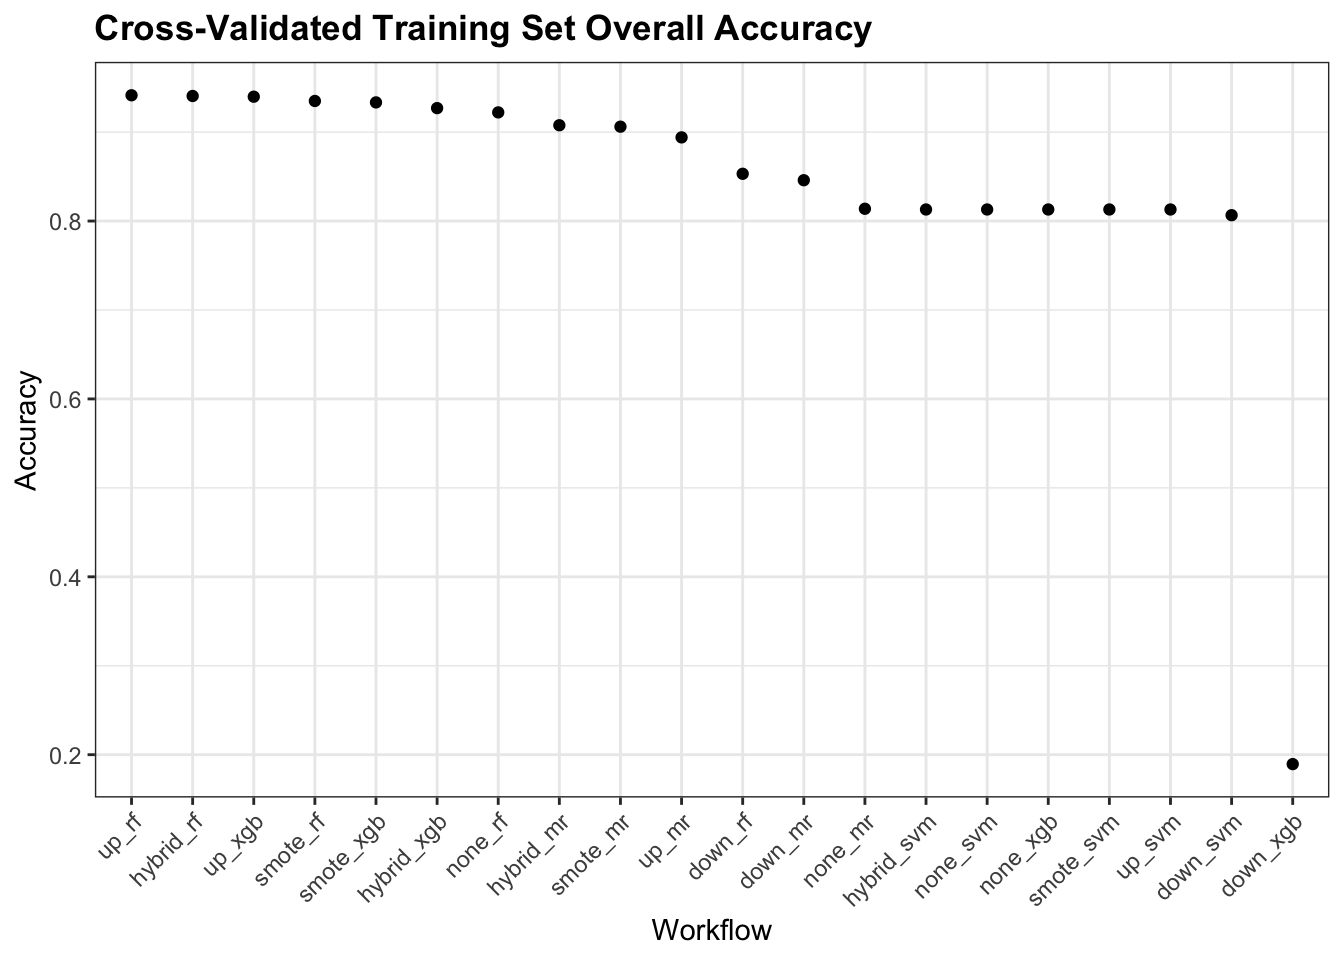
\includegraphics{OV_Histotypes_RSF_files/figure-latex/train-accuracy-1} 

}

\caption{Training Set Accuracy}\label{fig:train-accuracy}
\end{figure}

\begin{table}

\caption{\label{tab:train-accuracy-table}Training Set Accuracy by Algorithm and Subsampling Method}
\centering
\begin{tabular}[t]{l|l|l|l|l|l}
\hline
sampling & rf & svm & adaboost & mlr\_ridge & mlr\_lasso\\
\hline
none & 0.932 & 0.938 & 0.921 & 0.931 & 0.93\\
\hline
up & 0.937 & 0.936 & \textbf{0.94} & 0.893 & 0.903\\
\hline
down & 0.871 & 0.868 & 0.865 & 0.853 & 0.834\\
\hline
smote & 0.939 & 0.933 & 0.929 & 0.908 & 0.907\\
\hline
\end{tabular}
\end{table}

\begin{figure}[H]

{\centering 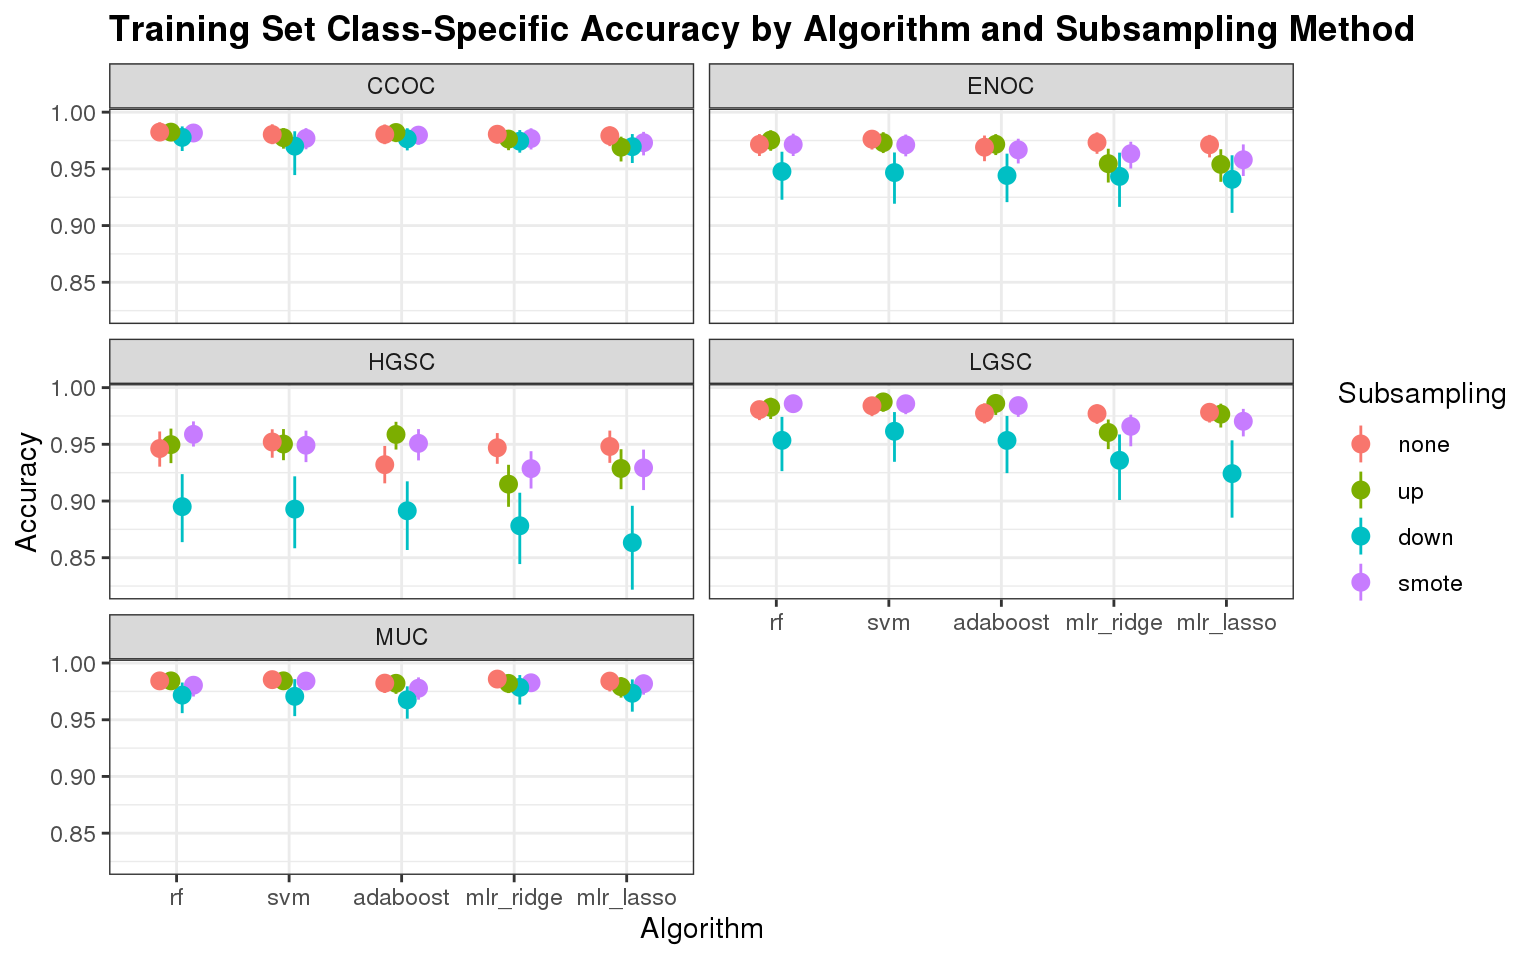
\includegraphics{OV_Histotypes_RSF_files/figure-latex/train-accuracy-class-1} 

}

\caption{Training Set Class-Specific Accuracy}\label{fig:train-accuracy-class}
\end{figure}

\begin{table}

\caption{\label{tab:train-accuracy-class-table}Training Set Class-Specific Accuracy by Algorithm and Subsampling Method}
\centering
\begin{tabular}[t]{l|l|l|l|l|l|l}
\hline
sampling & histotype & rf & svm & adaboost & mlr\_ridge & mlr\_lasso\\
\hline
none & CCOC & 0.982 & 0.98 & 0.98 & 0.981 & 0.979\\
\hline
none & ENOC & 0.972 & 0.976 & 0.969 & 0.973 & 0.971\\
\hline
none & HGSC & 0.946 & 0.952 & 0.932 & 0.947 & 0.948\\
\hline
none & LGSC & 0.981 & 0.984 & 0.978 & 0.977 & 0.978\\
\hline
none & MUC & 0.984 & 0.985 & 0.982 & 0.986 & 0.984\\
\hline
up & CCOC & 0.982 & 0.978 & 0.982 & 0.976 & 0.969\\
\hline
up & ENOC & 0.975 & 0.973 & 0.972 & 0.955 & 0.954\\
\hline
up & HGSC & 0.95 & 0.95 & 0.959 & 0.915 & 0.929\\
\hline
up & LGSC & 0.983 & \textbf{0.987} & 0.986 & 0.96 & 0.977\\
\hline
up & MUC & 0.984 & 0.984 & 0.982 & 0.982 & 0.979\\
\hline
down & CCOC & 0.978 & 0.97 & 0.976 & 0.974 & 0.97\\
\hline
down & ENOC & 0.948 & 0.947 & 0.944 & 0.943 & 0.941\\
\hline
down & HGSC & 0.895 & 0.893 & 0.891 & 0.878 & 0.863\\
\hline
down & LGSC & 0.953 & 0.962 & 0.953 & 0.936 & 0.924\\
\hline
down & MUC & 0.972 & 0.971 & 0.968 & 0.979 & 0.973\\
\hline
smote & CCOC & 0.982 & 0.977 & 0.98 & 0.977 & 0.973\\
\hline
smote & ENOC & 0.971 & 0.971 & 0.967 & 0.963 & 0.958\\
\hline
smote & HGSC & 0.959 & 0.949 & 0.951 & 0.929 & 0.929\\
\hline
smote & LGSC & 0.986 & 0.986 & 0.984 & 0.966 & 0.97\\
\hline
smote & MUC & 0.98 & 0.984 & 0.978 & 0.983 & 0.982\\
\hline
\end{tabular}
\end{table}

\hypertarget{f1-score}{%
\subsection{F1-Score}\label{f1-score}}

\begin{figure}[H]

{\centering 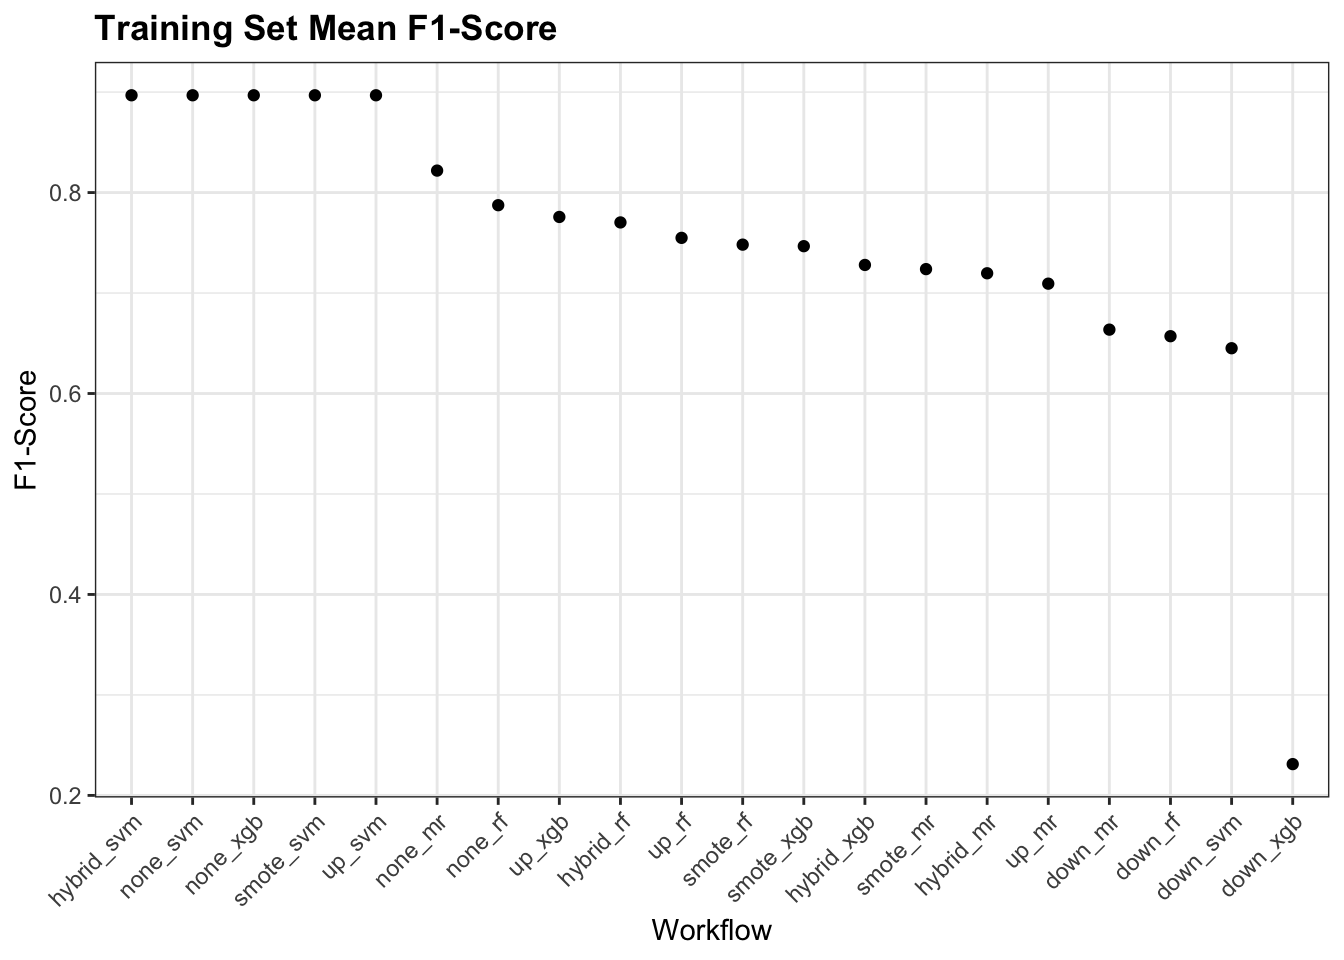
\includegraphics{OV_Histotypes_RSF_files/figure-latex/train-f1-1} 

}

\caption{Training Set F1-Score}\label{fig:train-f1}
\end{figure}

\begin{table}

\caption{\label{tab:train-f1-table}Training Set Macro-Averaged F1-Score by Algorithm and Subsampling Method}
\centering
\begin{tabular}[t]{l|l|l|l|l|l}
\hline
sampling & rf & svm & adaboost & mlr\_ridge & mlr\_lasso\\
\hline
none & 0.755 & 0.82 & 0.711 & 0.76 & 0.772\\
\hline
up & 0.791 & 0.818 & 0.821 & 0.762 & 0.759\\
\hline
down & 0.73 & 0.727 & 0.718 & 0.717 & 0.687\\
\hline
smote & \textbf{0.824} & 0.817 & 0.81 & 0.777 & 0.769\\
\hline
\end{tabular}
\end{table}

\begin{figure}[H]

{\centering 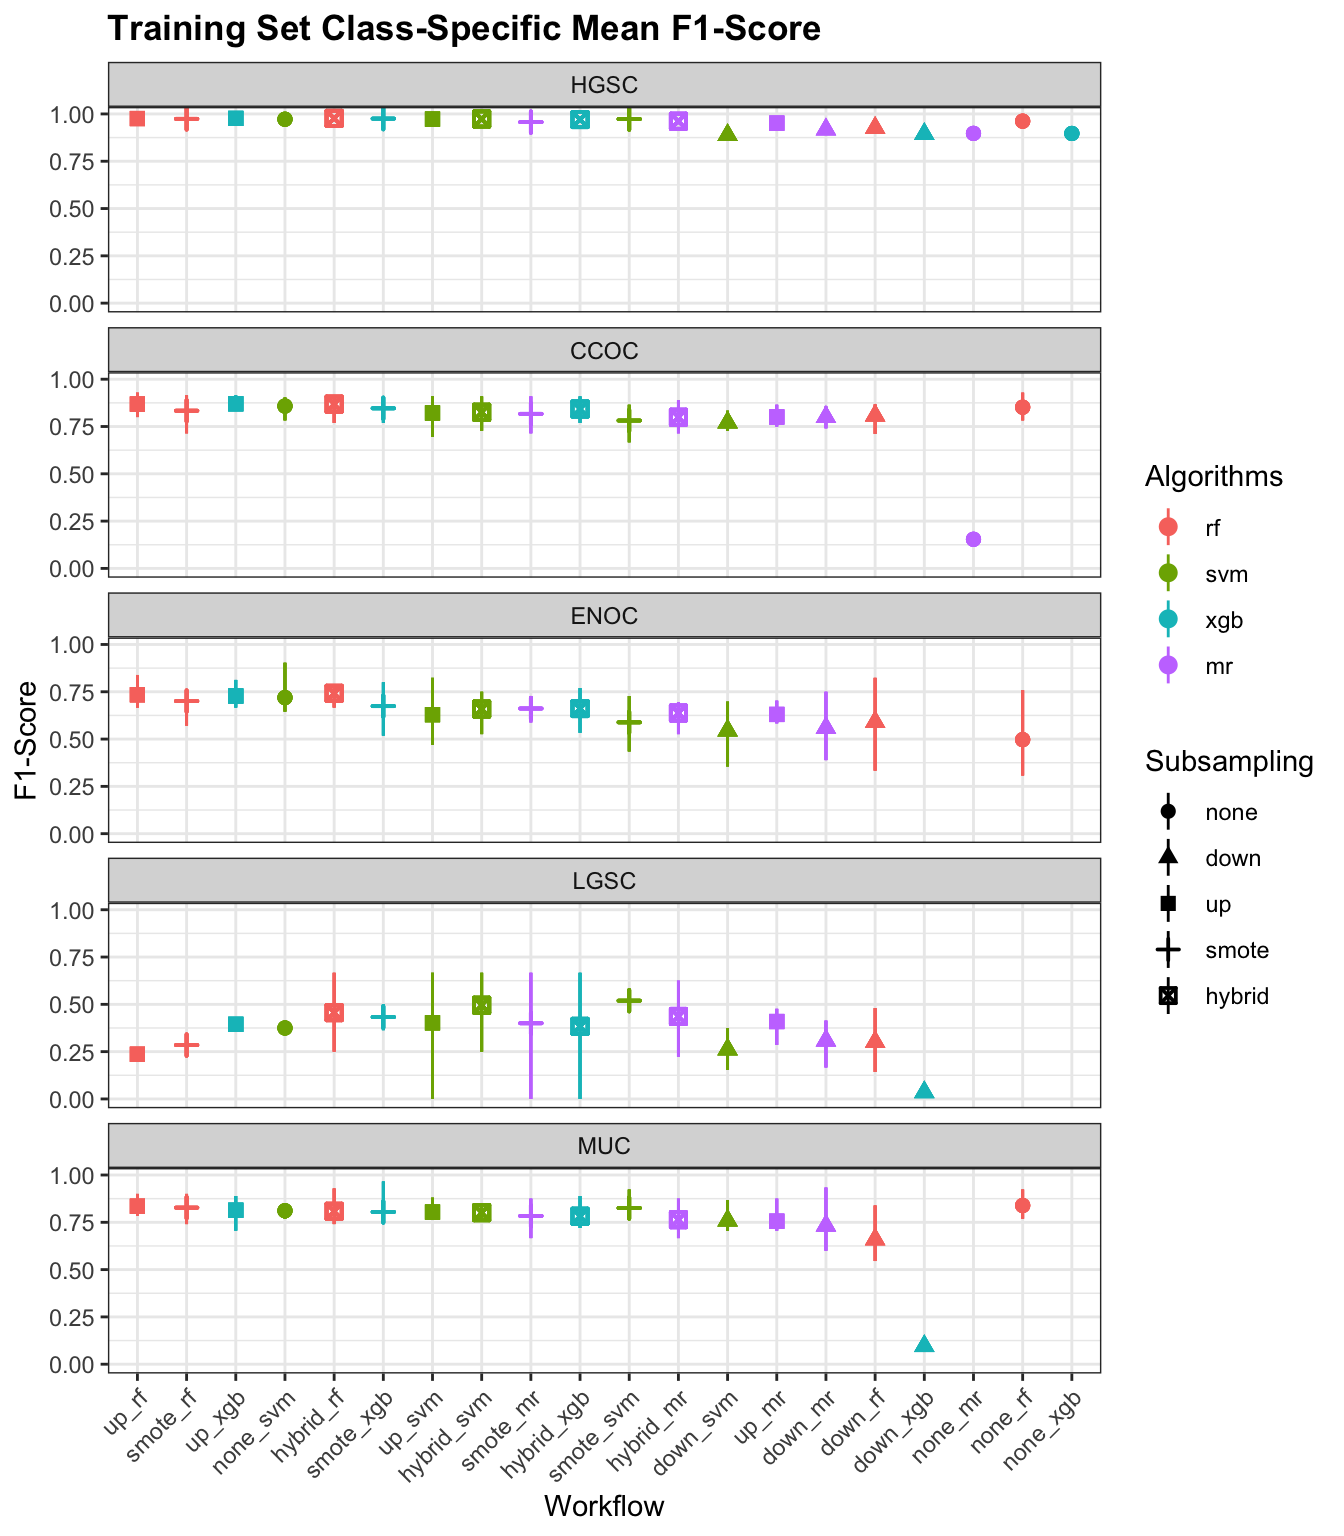
\includegraphics{OV_Histotypes_RSF_files/figure-latex/train-f1-class-1} 

}

\caption{Training Set Class-Specific F1-Score}\label{fig:train-f1-class}
\end{figure}

\begin{table}

\caption{\label{tab:train-f1-class-table}Training Set Class-Specific F1-Score by Algorithm and Subsampling Method}
\centering
\begin{tabular}[t]{l|l|l|l|l|l|l}
\hline
sampling & histotype & rf & svm & adaboost & mlr\_ridge & mlr\_lasso\\
\hline
none & CCOC & 0.866 & 0.848 & 0.846 & 0.853 & 0.843\\
\hline
none & ENOC & 0.724 & 0.786 & 0.681 & 0.757 & 0.74\\
\hline
none & HGSC & 0.967 & 0.97 & 0.959 & 0.967 & 0.968\\
\hline
none & LGSC & 0.375 & 0.667 & 0.2 & 0.353 & 0.471\\
\hline
none & MUC & 0.852 & 0.857 & 0.827 & 0.872 & 0.849\\
\hline
up & CCOC & 0.864 & 0.822 & 0.865 & 0.833 & 0.778\\
\hline
up & ENOC & 0.767 & 0.75 & 0.754 & 0.667 & 0.638\\
\hline
up & HGSC & 0.969 & 0.969 & \textbf{0.974} & 0.944 & 0.954\\
\hline
up & LGSC & 0.522 & 0.714 & 0.69 & 0.524 & 0.611\\
\hline
up & MUC & 0.852 & 0.846 & 0.839 & 0.841 & 0.808\\
\hline
down & CCOC & 0.841 & 0.79 & 0.833 & 0.821 & 0.792\\
\hline
down & ENOC & 0.641 & 0.629 & 0.615 & 0.627 & 0.605\\
\hline
down & HGSC & 0.93 & 0.928 & 0.927 & 0.917 & 0.907\\
\hline
down & LGSC & 0.487 & 0.526 & 0.481 & 0.413 & 0.368\\
\hline
down & MUC & 0.765 & 0.762 & 0.741 & 0.811 & 0.769\\
\hline
smote & CCOC & 0.862 & 0.824 & 0.85 & 0.835 & 0.813\\
\hline
smote & ENOC & 0.759 & 0.759 & 0.721 & 0.71 & 0.675\\
\hline
smote & HGSC & \textbf{0.974} & 0.968 & 0.969 & 0.953 & 0.954\\
\hline
smote & LGSC & 0.71 & 0.706 & 0.706 & 0.545 & 0.571\\
\hline
smote & MUC & 0.829 & 0.847 & 0.81 & 0.847 & 0.833\\
\hline
\end{tabular}
\end{table}

\hypertarget{kappa}{%
\subsection{Kappa}\label{kappa}}

\begin{figure}[H]

{\centering 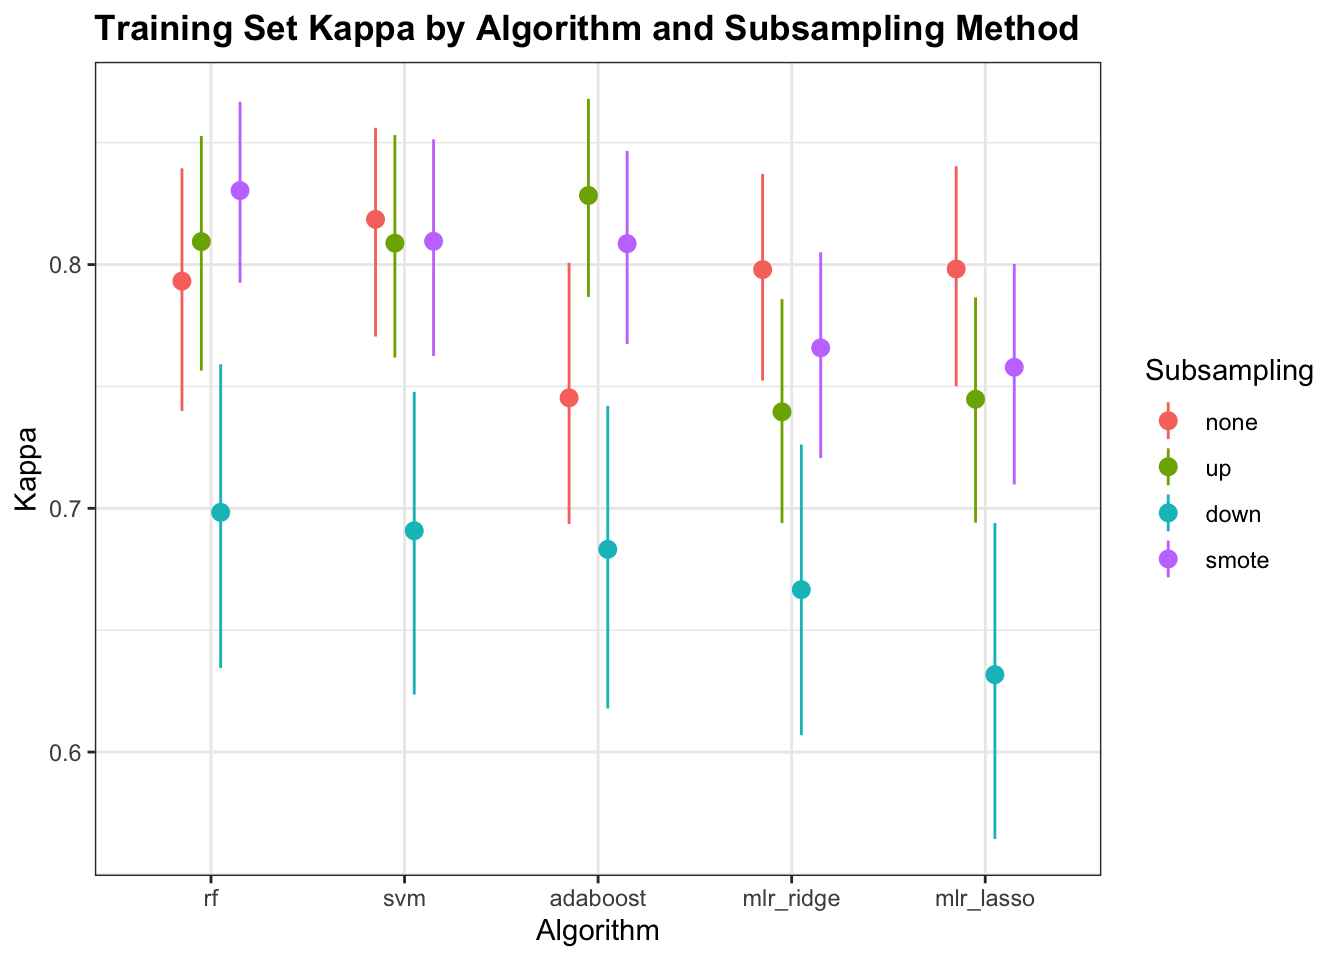
\includegraphics{OV_Histotypes_RSF_files/figure-latex/train-kappa-1} 

}

\caption{Training Set Kappa}\label{fig:train-kappa}
\end{figure}

\begin{table}

\caption{\label{tab:train-kappa-table}Training Set Kappa by Algorithm and Subsampling Method}
\centering
\begin{tabular}[t]{l|l|l|l|l|l}
\hline
sampling & rf & svm & adaboost & mlr\_ridge & mlr\_lasso\\
\hline
none & 0.793 & 0.819 & 0.745 & 0.798 & 0.798\\
\hline
up & 0.809 & 0.809 & 0.828 & 0.74 & 0.745\\
\hline
down & 0.698 & 0.691 & 0.683 & 0.667 & 0.632\\
\hline
smote & \textbf{0.83} & 0.81 & 0.809 & 0.766 & 0.758\\
\hline
\end{tabular}
\end{table}

\begin{figure}[H]

{\centering 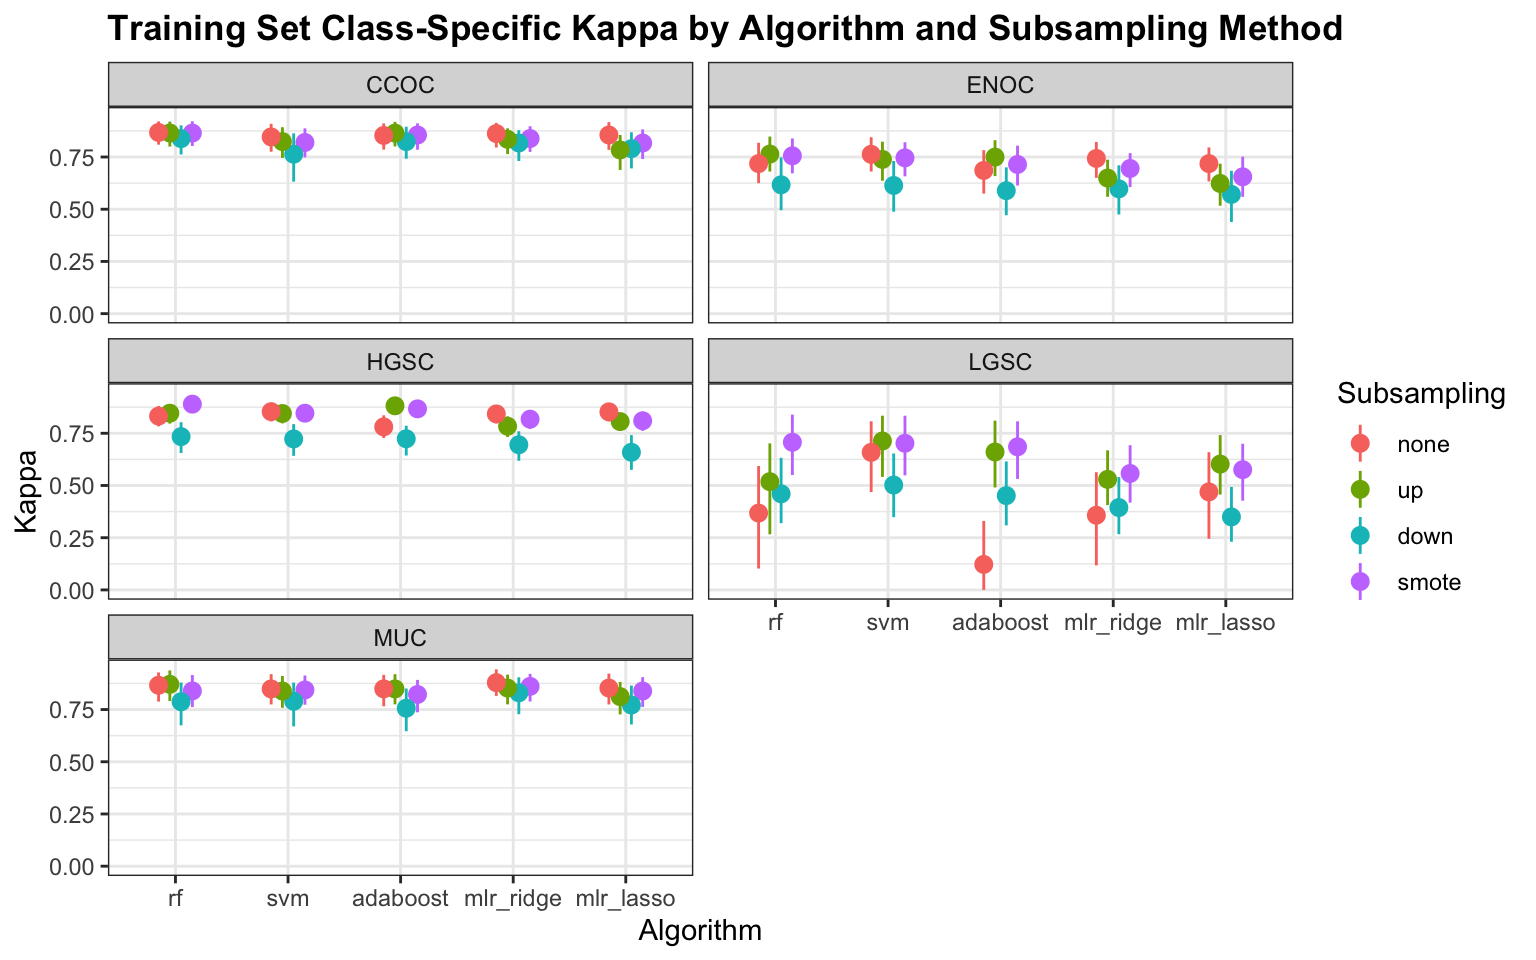
\includegraphics{OV_Histotypes_RSF_files/figure-latex/train-kappa-class-1} 

}

\caption{Training Set Class-Specific Kappa}\label{fig:train-kappa-class}
\end{figure}

\begin{table}

\caption{\label{tab:train-kappa-class-table}Training Set Class-Specific Kappa by Algorithm and Subsampling Method}
\centering
\begin{tabular}[t]{l|l|l|l|l|l|l}
\hline
sampling & histotype & rf & svm & adaboost & mlr\_ridge & mlr\_lasso\\
\hline
none & CCOC & 0.857 & 0.836 & 0.835 & 0.843 & 0.831\\
\hline
none & ENOC & 0.71 & 0.774 & 0.666 & 0.744 & 0.723\\
\hline
none & HGSC & 0.822 & 0.848 & 0.77 & 0.829 & 0.837\\
\hline
none & LGSC & 0.369 & 0.656 & 0.151 & 0.344 & 0.464\\
\hline
none & MUC & 0.844 & 0.849 & 0.818 & 0.864 & 0.839\\
\hline
up & CCOC & 0.854 & 0.812 & 0.855 & 0.82 & 0.762\\
\hline
up & ENOC & 0.753 & 0.735 & 0.739 & 0.645 & 0.614\\
\hline
up & HGSC & 0.835 & 0.839 & 0.873 & 0.768 & 0.792\\
\hline
up & LGSC & 0.514 & 0.707 & 0.682 & 0.508 & 0.599\\
\hline
up & MUC & 0.844 & 0.839 & 0.829 & 0.83 & 0.797\\
\hline
down & CCOC & 0.828 & 0.774 & 0.821 & 0.807 & 0.775\\
\hline
down & ENOC & 0.615 & 0.6 & 0.586 & 0.598 & 0.575\\
\hline
down & HGSC & 0.724 & 0.719 & 0.715 & 0.686 & 0.656\\
\hline
down & LGSC & 0.465 & 0.509 & 0.461 & 0.387 & 0.341\\
\hline
down & MUC & 0.75 & 0.746 & 0.723 & 0.798 & 0.755\\
\hline
smote & CCOC & 0.853 & 0.81 & 0.839 & 0.822 & 0.798\\
\hline
smote & ENOC & 0.744 & 0.743 & 0.704 & 0.69 & 0.651\\
\hline
smote & HGSC & \textbf{0.876} & 0.842 & 0.854 & 0.8 & 0.798\\
\hline
smote & LGSC & 0.701 & 0.697 & 0.696 & 0.528 & 0.559\\
\hline
smote & MUC & 0.817 & 0.839 & 0.797 & 0.839 & 0.824\\
\hline
\end{tabular}
\end{table}

\hypertarget{g-mean}{%
\subsection{G-mean}\label{g-mean}}

\begin{figure}[H]

{\centering 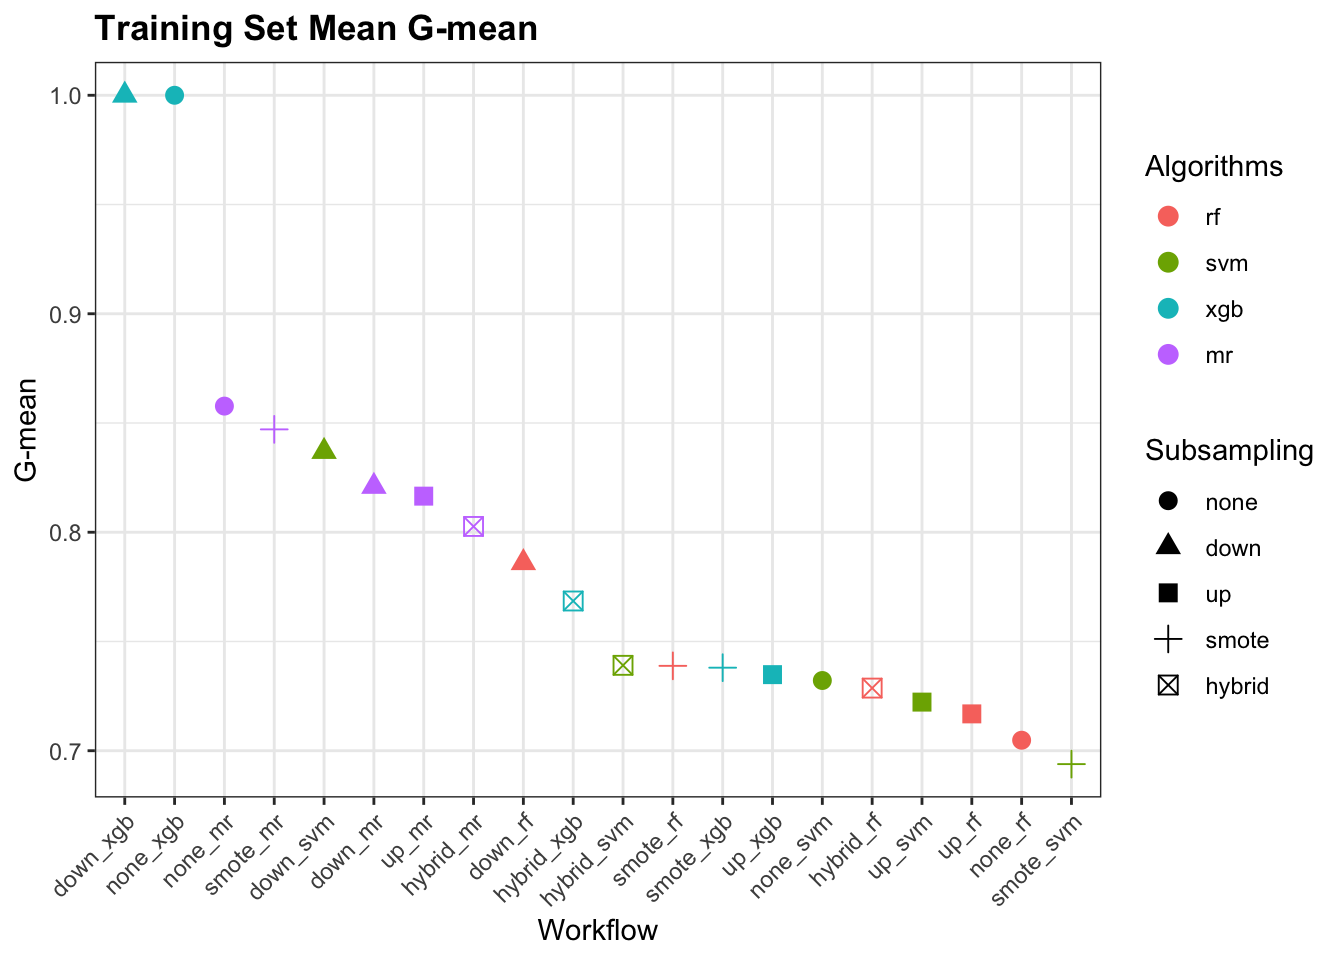
\includegraphics{OV_Histotypes_RSF_files/figure-latex/train-gmean-1} 

}

\caption{Training Set G-mean}\label{fig:train-gmean}
\end{figure}

\begin{table}

\caption{\label{tab:train-gmean-table}Training Set G-mean by Algorithm and Subsampling Method}
\centering
\begin{tabular}[t]{l|l|l|l|l|l}
\hline
sampling & rf & svm & adaboost & mlr\_ridge & mlr\_lasso\\
\hline
none & 0.632 & 0.779 & 0.497 & 0.654 & 0.71\\
\hline
up & 0.701 & 0.766 & 0.8 & \textbf{0.868} & 0.799\\
\hline
down & 0.851 & 0.843 & 0.841 & 0.856 & 0.832\\
\hline
smote & 0.828 & 0.801 & 0.831 & 0.852 & 0.835\\
\hline
\end{tabular}
\end{table}

\begin{figure}[H]

{\centering \includegraphics{OV_Histotypes_RSF_files/figure-latex/train-gmean-class-1} 

}

\caption{Training Set Class-Specific G-mean}\label{fig:train-gmean-class}
\end{figure}

\begin{table}

\caption{\label{tab:train-gmean-class-table}Training Set Class-Specific G-mean by Algorithm and Subsampling Method}
\centering
\begin{tabular}[t]{l|l|l|l|l|l|l}
\hline
sampling & histotype & rf & svm & adaboost & mlr\_ridge & mlr\_lasso\\
\hline
none & CCOC & 0.896 & 0.892 & 0.876 & 0.896 & 0.9\\
\hline
none & ENOC & 0.796 & 0.857 & 0.753 & 0.843 & 0.836\\
\hline
none & HGSC & 0.873 & 0.903 & 0.83 & 0.888 & 0.901\\
\hline
none & LGSC & 0.499 & 0.785 & 0.289 & 0.5 & 0.622\\
\hline
none & MUC & 0.912 & 0.901 & 0.881 & 0.926 & 0.918\\
\hline
up & CCOC & 0.893 & 0.864 & 0.906 & 0.921 & 0.885\\
\hline
up & ENOC & 0.835 & 0.83 & 0.86 & 0.878 & 0.831\\
\hline
up & HGSC & 0.883 & 0.891 & 0.93 & 0.93 & 0.918\\
\hline
up & LGSC & 0.612 & 0.813 & 0.794 & 0.933 & 0.867\\
\hline
up & MUC & 0.906 & 0.889 & 0.927 & 0.935 & 0.902\\
\hline
down & CCOC & 0.921 & 0.903 & 0.914 & 0.912 & 0.911\\
\hline
down & ENOC & 0.878 & 0.869 & 0.854 & 0.879 & 0.858\\
\hline
down & HGSC & 0.917 & 0.914 & 0.914 & 0.908 & 0.898\\
\hline
down & LGSC & 0.912 & 0.916 & 0.909 & 0.928 & 0.908\\
\hline
down & MUC & 0.921 & 0.919 & 0.923 & 0.927 & 0.912\\
\hline
smote & CCOC & 0.92 & 0.885 & 0.913 & 0.919 & 0.916\\
\hline
smote & ENOC & 0.875 & 0.865 & 0.861 & 0.874 & 0.858\\
\hline
smote & HGSC & \textbf{0.943} & 0.912 & 0.939 & 0.933 & 0.929\\
\hline
smote & LGSC & 0.842 & 0.841 & 0.871 & 0.91 & 0.886\\
\hline
smote & MUC & 0.927 & 0.9 & 0.928 & 0.933 & 0.926\\
\hline
\end{tabular}
\end{table}

\hypertarget{cs1-set}{%
\section{CS1 Set}\label{cs1-set}}

\hypertarget{accuracy-1}{%
\subsection{Accuracy}\label{accuracy-1}}

\begin{figure}[H]

{\centering \includegraphics{OV_Histotypes_RSF_files/figure-latex/cs1-accuracy-1} 

}

\caption{CS1 Set Accuracy}\label{fig:cs1-accuracy}
\end{figure}

\begin{table}

\caption{\label{tab:cs1-accuracy-table}CS1 Set Accuracy by Algorithm and Subsampling Method}
\centering
\begin{tabular}[t]{l|l|l|l|l|l}
\hline
sampling & rf & svm & adaboost & mlr\_ridge & mlr\_lasso\\
\hline
none & 0.816 & \textbf{0.842} & 0.8 & 0.832 & 0.823\\
\hline
up & 0.835 & 0.833 & 0.825 & 0.83 & 0.814\\
\hline
down & 0.798 & 0.802 & 0.776 & 0.788 & 0.764\\
\hline
smote & 0.837 & 0.837 & 0.828 & 0.83 & 0.814\\
\hline
\end{tabular}
\end{table}

\begin{figure}[H]

{\centering \includegraphics{OV_Histotypes_RSF_files/figure-latex/cs1-accuracy-class-1} 

}

\caption{CS1 Set Class-Specific Accuracy}\label{fig:cs1-accuracy-class}
\end{figure}

\begin{table}

\caption{\label{tab:cs1-accuracy-class-table}CS1 Set Class-Specific Accuracy by Algorithm and Subsampling Method}
\centering
\begin{tabular}[t]{l|l|l|l|l|l|l}
\hline
sampling & histotype & rf & svm & adaboost & mlr\_ridge & mlr\_lasso\\
\hline
none & CCOC & 0.939 & 0.943 & 0.939 & 0.935 & 0.931\\
\hline
none & ENOC & 0.894 & 0.917 & 0.892 & 0.902 & 0.9\\
\hline
none & HGSC & 0.891 & 0.894 & 0.87 & 0.903 & 0.896\\
\hline
none & LGSC & 0.95 & 0.969 & 0.943 & 0.96 & 0.957\\
\hline
none & MUC & 0.966 & 0.962 & 0.96 & 0.969 & 0.969\\
\hline
up & CCOC & 0.942 & 0.938 & 0.939 & 0.927 & 0.918\\
\hline
up & ENOC & 0.902 & 0.906 & 0.897 & 0.899 & 0.885\\
\hline
up & HGSC & 0.907 & 0.894 & 0.897 & 0.908 & 0.903\\
\hline
up & LGSC & 0.96 & \textbf{0.971} & 0.958 & 0.959 & 0.958\\
\hline
up & MUC & 0.967 & 0.963 & 0.961 & 0.968 & 0.969\\
\hline
down & CCOC & 0.936 & 0.938 & 0.932 & 0.937 & 0.922\\
\hline
down & ENOC & 0.887 & 0.895 & 0.876 & 0.892 & 0.878\\
\hline
down & HGSC & 0.883 & 0.874 & 0.869 & 0.872 & 0.858\\
\hline
down & LGSC & 0.939 & 0.949 & 0.935 & 0.925 & 0.921\\
\hline
down & MUC & 0.958 & 0.954 & 0.95 & 0.96 & 0.957\\
\hline
smote & CCOC & 0.94 & 0.939 & 0.939 & 0.929 & 0.926\\
\hline
smote & ENOC & 0.892 & 0.905 & 0.888 & 0.896 & 0.891\\
\hline
smote & HGSC & 0.916 & 0.897 & 0.905 & 0.907 & 0.894\\
\hline
smote & LGSC & 0.961 & 0.97 & 0.963 & 0.96 & 0.957\\
\hline
smote & MUC & 0.962 & 0.967 & 0.96 & 0.968 & 0.969\\
\hline
\end{tabular}
\end{table}

\hypertarget{f1-score-1}{%
\subsection{F1-Score}\label{f1-score-1}}

\begin{figure}[H]

{\centering \includegraphics{OV_Histotypes_RSF_files/figure-latex/cs1-f1-1} 

}

\caption{CS1 Set F1-Score}\label{fig:cs1-f1}
\end{figure}

\begin{table}

\caption{\label{tab:cs1-f1-table}CS1 Set Macro-Averaged F1-Score by Algorithm and Subsampling Method}
\centering
\begin{tabular}[t]{l|l|l|l|l|l}
\hline
sampling & rf & svm & adaboost & mlr\_ridge & mlr\_lasso\\
\hline
none & 0.731 & \textbf{0.791} & 0.707 & 0.771 & 0.761\\
\hline
up & 0.77 & 0.781 & 0.755 & 0.786 & 0.77\\
\hline
down & 0.746 & 0.754 & 0.728 & 0.745 & 0.716\\
\hline
smote & 0.779 & 0.789 & 0.773 & 0.784 & 0.773\\
\hline
\end{tabular}
\end{table}

\begin{figure}[H]

{\centering \includegraphics{OV_Histotypes_RSF_files/figure-latex/cs1-f1-class-1} 

}

\caption{CS1 Set Class-Specific F1-Score}\label{fig:cs1-f1-class}
\end{figure}

\begin{table}

\caption{\label{tab:cs1-f1-class-table}CS1 Set Class-Specific F1-Score by Algorithm and Subsampling Method}
\centering
\begin{tabular}[t]{l|l|l|l|l|l|l}
\hline
sampling & histotype & rf & svm & adaboost & mlr\_ridge & mlr\_lasso\\
\hline
none & CCOC & 0.824 & 0.828 & 0.824 & 0.812 & 0.8\\
\hline
none & ENOC & 0.762 & 0.8 & 0.745 & 0.769 & 0.772\\
\hline
none & HGSC & 0.889 & 0.893 & 0.873 & 0.9 & 0.891\\
\hline
none & LGSC & 0.5 & 0.75 & 0.4 & 0.667 & 0.615\\
\hline
none & MUC & 0.667 & 0.714 & 0.667 & 0.75 & 0.75\\
\hline
up & CCOC & 0.833 & 0.815 & 0.824 & 0.8 & 0.773\\
\hline
up & ENOC & 0.78 & 0.783 & 0.765 & 0.769 & 0.744\\
\hline
up & HGSC & 0.905 & 0.893 & 0.895 & 0.901 & 0.891\\
\hline
up & LGSC & 0.667 & 0.769 & 0.615 & 0.727 & 0.714\\
\hline
up & MUC & 0.727 & 0.667 & 0.714 & 0.75 & 0.762\\
\hline
down & CCOC & 0.822 & 0.824 & 0.811 & 0.821 & 0.786\\
\hline
down & ENOC & 0.75 & 0.769 & 0.718 & 0.762 & 0.723\\
\hline
down & HGSC & 0.864 & 0.857 & 0.85 & 0.851 & 0.835\\
\hline
down & LGSC & 0.632 & 0.667 & 0.615 & 0.588 & 0.571\\
\hline
down & MUC & 0.706 & 0.706 & 0.667 & 0.714 & 0.667\\
\hline
smote & CCOC & 0.829 & 0.828 & 0.828 & 0.81 & 0.789\\
\hline
smote & ENOC & 0.769 & 0.783 & 0.756 & 0.766 & 0.757\\
\hline
smote & HGSC & \textbf{0.909} & 0.892 & 0.899 & 0.897 & 0.884\\
\hline
smote & LGSC & 0.714 & 0.75 & 0.714 & 0.727 & 0.706\\
\hline
smote & MUC & 0.727 & 0.714 & 0.706 & 0.75 & 0.762\\
\hline
\end{tabular}
\end{table}

\hypertarget{kappa-1}{%
\subsection{Kappa}\label{kappa-1}}

\begin{figure}[H]

{\centering \includegraphics{OV_Histotypes_RSF_files/figure-latex/cs1-kappa-1} 

}

\caption{CS1 Set Kappa}\label{fig:cs1-kappa}
\end{figure}

\begin{table}

\caption{\label{tab:cs1-kappa-table}CS1 Set Kappa by Algorithm and Subsampling Method}
\centering
\begin{tabular}[t]{l|l|l|l|l|l}
\hline
sampling & rf & svm & adaboost & mlr\_ridge & mlr\_lasso\\
\hline
none & 0.724 & \textbf{0.767} & 0.697 & 0.752 & 0.74\\
\hline
up & 0.756 & 0.752 & 0.741 & 0.757 & 0.732\\
\hline
down & 0.716 & 0.72 & 0.687 & 0.706 & 0.673\\
\hline
smote & 0.763 & 0.759 & 0.751 & 0.755 & 0.736\\
\hline
\end{tabular}
\end{table}

\begin{figure}[H]

{\centering \includegraphics{OV_Histotypes_RSF_files/figure-latex/cs1-kappa-class-1} 

}

\caption{CS1 Set Class-Specific Kappa}\label{fig:cs1-kappa-class}
\end{figure}

\begin{table}

\caption{\label{tab:cs1-kappa-class-table}CS1 Set Class-Specific Kappa by Algorithm and Subsampling Method}
\centering
\begin{tabular}[t]{l|l|l|l|l|l|l}
\hline
sampling & histotype & rf & svm & adaboost & mlr\_ridge & mlr\_lasso\\
\hline
none & CCOC & 0.786 & 0.794 & 0.785 & 0.773 & 0.764\\
\hline
none & ENOC & 0.693 & 0.75 & 0.678 & 0.707 & 0.704\\
\hline
none & HGSC & 0.781 & 0.787 & 0.741 & 0.806 & 0.792\\
\hline
none & LGSC & 0.477 & 0.728 & 0.273 & 0.646 & 0.587\\
\hline
none & MUC & 0.652 & 0.693 & 0.647 & 0.729 & 0.739\\
\hline
up & CCOC & 0.797 & 0.777 & 0.787 & 0.76 & 0.718\\
\hline
up & ENOC & 0.718 & 0.723 & 0.699 & 0.702 & 0.669\\
\hline
up & HGSC & 0.814 & 0.788 & 0.795 & 0.816 & 0.802\\
\hline
up & LGSC & 0.647 & 0.753 & 0.585 & 0.696 & 0.692\\
\hline
up & MUC & 0.71 & 0.647 & 0.692 & 0.739 & 0.74\\
\hline
down & CCOC & 0.784 & 0.786 & 0.767 & 0.778 & 0.735\\
\hline
down & ENOC & 0.674 & 0.701 & 0.636 & 0.69 & 0.647\\
\hline
down & HGSC & 0.761 & 0.742 & 0.734 & 0.741 & 0.711\\
\hline
down & LGSC & 0.594 & 0.64 & 0.587 & 0.553 & 0.528\\
\hline
down & MUC & 0.678 & 0.675 & 0.647 & 0.693 & 0.65\\
\hline
smote & CCOC & 0.795 & 0.79 & 0.79 & 0.762 & 0.747\\
\hline
smote & ENOC & 0.699 & 0.725 & 0.678 & 0.7 & 0.685\\
\hline
smote & HGSC & \textbf{0.829} & 0.792 & 0.81 & 0.81 & 0.787\\
\hline
smote & LGSC & 0.691 & 0.74 & 0.694 & 0.711 & 0.676\\
\hline
smote & MUC & 0.709 & 0.694 & 0.678 & 0.73 & 0.74\\
\hline
\end{tabular}
\end{table}

\hypertarget{g-mean-1}{%
\subsection{G-mean}\label{g-mean-1}}

\begin{figure}[H]

{\centering \includegraphics{OV_Histotypes_RSF_files/figure-latex/cs1-gmean-1} 

}

\caption{CS1 Set G-mean}\label{fig:cs1-gmean}
\end{figure}

\begin{table}

\caption{\label{tab:cs1-gmean-table}CS1 Set G-mean by Algorithm and Subsampling Method}
\centering
\begin{tabular}[t]{l|l|l|l|l|l}
\hline
sampling & rf & svm & adaboost & mlr\_ridge & mlr\_lasso\\
\hline
none & 0.638 & 0.747 & 0.557 & 0.728 & 0.72\\
\hline
up & 0.713 & 0.718 & 0.703 & \textbf{0.794} & 0.769\\
\hline
down & 0.778 & 0.791 & 0.761 & 0.779 & 0.753\\
\hline
smote & 0.76 & 0.75 & 0.766 & 0.789 & 0.782\\
\hline
\end{tabular}
\end{table}

\begin{figure}[H]

{\centering \includegraphics{OV_Histotypes_RSF_files/figure-latex/cs1-gmean-class-1} 

}

\caption{CS1 Set Class-Specific G-mean}\label{fig:cs1-gmean-class}
\end{figure}

\begin{table}

\caption{\label{tab:cs1-gmean-class-table}CS1 Set Class-Specific G-mean by Algorithm and Subsampling Method}
\centering
\begin{tabular}[t]{l|l|l|l|l|l|l}
\hline
sampling & histotype & rf & svm & adaboost & mlr\_ridge & mlr\_lasso\\
\hline
none & CCOC & 0.889 & 0.889 & 0.884 & 0.889 & 0.879\\
\hline
none & ENOC & 0.854 & 0.868 & 0.831 & 0.845 & 0.851\\
\hline
none & HGSC & 0.892 & 0.896 & 0.871 & 0.905 & 0.896\\
\hline
none & LGSC & 0.577 & 0.812 & 0.408 & 0.707 & 0.707\\
\hline
none & MUC & 0.756 & 0.791 & 0.745 & 0.836 & 0.816\\
\hline
up & CCOC & 0.893 & 0.886 & 0.886 & 0.889 & 0.868\\
\hline
up & ENOC & 0.863 & 0.848 & 0.848 & 0.847 & 0.836\\
\hline
up & HGSC & 0.909 & 0.895 & 0.898 & 0.906 & 0.899\\
\hline
up & LGSC & 0.707 & 0.793 & 0.703 & 0.88 & 0.873\\
\hline
up & MUC & 0.812 & 0.745 & 0.808 & 0.866 & 0.853\\
\hline
down & CCOC & 0.896 & 0.889 & 0.89 & 0.897 & 0.883\\
\hline
down & ENOC & 0.847 & 0.859 & 0.817 & 0.848 & 0.823\\
\hline
down & HGSC & 0.873 & 0.866 & 0.861 & 0.862 & 0.848\\
\hline
down & LGSC & 0.871 & 0.865 & 0.866 & 0.877 & 0.851\\
\hline
down & MUC & 0.854 & 0.902 & 0.855 & 0.856 & 0.837\\
\hline
smote & CCOC & 0.895 & 0.892 & 0.893 & 0.889 & 0.887\\
\hline
smote & ENOC & 0.87 & 0.868 & 0.856 & 0.856 & 0.853\\
\hline
smote & HGSC & \textbf{0.913} & 0.897 & 0.904 & 0.902 & 0.89\\
\hline
smote & LGSC & 0.804 & 0.812 & 0.812 & 0.861 & 0.857\\
\hline
smote & MUC & 0.832 & 0.791 & 0.82 & 0.857 & 0.861\\
\hline
\end{tabular}
\end{table}

\hypertarget{cs2-set}{%
\section{CS2 Set}\label{cs2-set}}

\hypertarget{accuracy-2}{%
\subsection{Accuracy}\label{accuracy-2}}

\begin{figure}[H]

{\centering \includegraphics{OV_Histotypes_RSF_files/figure-latex/cs2-accuracy-1} 

}

\caption{CS2 Set Accuracy}\label{fig:cs2-accuracy}
\end{figure}

\begin{table}

\caption{\label{tab:cs2-accuracy-table}CS2 Set Accuracy by Algorithm and Subsampling Method}
\centering
\begin{tabular}[t]{l|l|l|l|l|l}
\hline
sampling & rf & svm & adaboost & mlr\_ridge & mlr\_lasso\\
\hline
none & 0.921 & 0.925 & 0.905 & \textbf{0.933} & 0.927\\
\hline
up & 0.925 & 0.923 & 0.93 & 0.918 & 0.916\\
\hline
down & 0.855 & 0.838 & 0.839 & 0.812 & 0.811\\
\hline
smote & 0.925 & 0.92 & 0.921 & 0.909 & 0.896\\
\hline
\end{tabular}
\end{table}

\begin{figure}[H]

{\centering \includegraphics{OV_Histotypes_RSF_files/figure-latex/cs2-accuracy-class-1} 

}

\caption{CS2 Set Class-Specific Accuracy}\label{fig:cs2-accuracy-class}
\end{figure}

\begin{table}

\caption{\label{tab:cs2-accuracy-class-table}CS2 Set Class-Specific Accuracy by Algorithm and Subsampling Method}
\centering
\begin{tabular}[t]{l|l|l|l|l|l|l}
\hline
sampling & histotype & rf & svm & adaboost & mlr\_ridge & mlr\_lasso\\
\hline
none & CCOC & 0.984 & 0.981 & 0.981 & \textbf{0.987} & 0.983\\
\hline
none & ENOC & 0.973 & 0.978 & 0.965 & 0.977 & 0.974\\
\hline
none & HGSC & 0.927 & 0.935 & 0.908 & 0.946 & 0.943\\
\hline
none & LGSC & 0.977 & 0.977 & 0.977 & 0.977 & 0.976\\
\hline
none & MUC & 0.981 & 0.978 & 0.98 & 0.983 & 0.98\\
\hline
up & CCOC & 0.986 & 0.98 & 0.986 & \textbf{0.987} & 0.986\\
\hline
up & ENOC & 0.977 & 0.979 & 0.98 & 0.967 & 0.966\\
\hline
up & HGSC & 0.93 & 0.93 & 0.94 & 0.935 & 0.936\\
\hline
up & LGSC & 0.977 & 0.98 & 0.978 & 0.971 & 0.972\\
\hline
up & MUC & 0.982 & 0.978 & 0.98 & 0.975 & 0.976\\
\hline
down & CCOC & 0.981 & 0.953 & 0.978 & 0.976 & 0.971\\
\hline
down & ENOC & 0.958 & 0.954 & 0.957 & 0.952 & 0.939\\
\hline
down & HGSC & 0.876 & 0.862 & 0.865 & 0.84 & 0.839\\
\hline
down & LGSC & 0.952 & 0.956 & 0.94 & 0.921 & 0.922\\
\hline
down & MUC & 0.95 & 0.96 & 0.946 & 0.945 & 0.961\\
\hline
smote & CCOC & 0.985 & 0.979 & 0.984 & 0.986 & 0.981\\
\hline
smote & ENOC & 0.975 & 0.977 & 0.974 & 0.963 & 0.957\\
\hline
smote & HGSC & 0.939 & 0.932 & 0.939 & 0.928 & 0.919\\
\hline
smote & LGSC & 0.98 & 0.98 & 0.98 & 0.97 & 0.964\\
\hline
smote & MUC & 0.972 & 0.975 & 0.968 & 0.974 & 0.973\\
\hline
\end{tabular}
\end{table}

\hypertarget{f1-score-2}{%
\subsection{F1-Score}\label{f1-score-2}}

\begin{figure}[H]

{\centering \includegraphics{OV_Histotypes_RSF_files/figure-latex/cs2-f1-1} 

}

\caption{CS2 Set F1-Score}\label{fig:cs2-f1}
\end{figure}

\begin{table}

\caption{\label{tab:cs2-f1-table}CS2 Set Macro-Averaged F1-Score by Algorithm and Subsampling Method}
\centering
\begin{tabular}[t]{l|l|l|l|l|l}
\hline
sampling & rf & svm & adaboost & mlr\_ridge & mlr\_lasso\\
\hline
none & 0.718 & 0.762 & 0.736 & 0.752 & 0.74\\
\hline
up & 0.719 & 0.751 & 0.74 & 0.773 & 0.754\\
\hline
down & 0.699 & 0.668 & 0.675 & 0.652 & 0.645\\
\hline
smote & \textbf{0.782} & 0.755 & 0.769 & 0.762 & 0.732\\
\hline
\end{tabular}
\end{table}

\begin{figure}[H]

{\centering \includegraphics{OV_Histotypes_RSF_files/figure-latex/cs2-f1-class-1} 

}

\caption{CS2 Set Class-Specific F1-Score}\label{fig:cs2-f1-class}
\end{figure}

\begin{table}

\caption{\label{tab:cs2-f1-class-table}CS2 Set Class-Specific F1-Score by Algorithm and Subsampling Method}
\centering
\begin{tabular}[t]{l|l|l|l|l|l|l}
\hline
sampling & histotype & rf & svm & adaboost & mlr\_ridge & mlr\_lasso\\
\hline
none & CCOC & 0.889 & 0.857 & 0.857 & 0.905 & 0.878\\
\hline
none & ENOC & 0.5 & 0.667 & 0.222 & 0.636 & 0.609\\
\hline
none & HGSC & 0.955 & 0.96 & 0.945 & \textbf{0.966} & 0.964\\
\hline
none & LGSC & 0.222 & 0.5 & 0.268 & 0.364 & 0.4\\
\hline
none & MUC & 0.87 & 0.842 & 0.851 & 0.875 & 0.863\\
\hline
up & CCOC & 0.894 & 0.842 & 0.9 & 0.909 & 0.896\\
\hline
up & ENOC & 0.571 & 0.667 & 0.667 & 0.606 & 0.581\\
\hline
up & HGSC & 0.958 & 0.957 & 0.963 & 0.958 & 0.959\\
\hline
up & LGSC & 0.25 & 0.5 & 0.308 & 0.571 & 0.526\\
\hline
up & MUC & 0.864 & 0.833 & 0.86 & 0.84 & 0.837\\
\hline
down & CCOC & 0.875 & 0.739 & 0.863 & 0.84 & 0.809\\
\hline
down & ENOC & 0.563 & 0.519 & 0.545 & 0.515 & 0.452\\
\hline
down & HGSC & 0.916 & 0.907 & 0.908 & 0.888 & 0.89\\
\hline
down & LGSC & 0.435 & 0.444 & 0.375 & 0.341 & 0.34\\
\hline
down & MUC & 0.72 & 0.742 & 0.7 & 0.696 & 0.75\\
\hline
smote & CCOC & 0.9 & 0.839 & 0.898 & 0.903 & 0.872\\
\hline
smote & ENOC & 0.667 & 0.632 & 0.645 & 0.581 & 0.533\\
\hline
smote & HGSC & 0.961 & 0.958 & 0.961 & 0.953 & 0.947\\
\hline
smote & LGSC & 0.556 & 0.545 & 0.556 & 0.545 & 0.5\\
\hline
smote & MUC & 0.821 & 0.818 & 0.8 & 0.833 & 0.824\\
\hline
\end{tabular}
\end{table}

\hypertarget{kappa-2}{%
\subsection{Kappa}\label{kappa-2}}

\begin{figure}[H]

{\centering \includegraphics{OV_Histotypes_RSF_files/figure-latex/cs2-kappa-1} 

}

\caption{CS2 Set Kappa}\label{fig:cs2-kappa}
\end{figure}

\begin{table}

\caption{\label{tab:cs2-kappa-table}CS2 Set Kappa by Algorithm and Subsampling Method}
\centering
\begin{tabular}[t]{l|l|l|l|l|l}
\hline
sampling & rf & svm & adaboost & mlr\_ridge & mlr\_lasso\\
\hline
none & 0.75 & 0.774 & 0.678 & \textbf{0.803} & 0.788\\
\hline
up & 0.763 & 0.76 & 0.791 & 0.787 & 0.775\\
\hline
down & 0.67 & 0.629 & 0.642 & 0.601 & 0.594\\
\hline
smote & 0.798 & 0.762 & 0.788 & 0.77 & 0.736\\
\hline
\end{tabular}
\end{table}

\begin{figure}[H]

{\centering \includegraphics{OV_Histotypes_RSF_files/figure-latex/cs2-kappa-class-1} 

}

\caption{CS2 Set Class-Specific Kappa}\label{fig:cs2-kappa-class}
\end{figure}

\begin{table}

\caption{\label{tab:cs2-kappa-class-table}CS2 Set Class-Specific Kappa by Algorithm and Subsampling Method}
\centering
\begin{tabular}[t]{l|l|l|l|l|l|l}
\hline
sampling & histotype & rf & svm & adaboost & mlr\_ridge & mlr\_lasso\\
\hline
none & CCOC & 0.88 & 0.849 & 0.846 & 0.897 & 0.869\\
\hline
none & ENOC & 0.484 & 0.661 & 0.162 & 0.623 & 0.595\\
\hline
none & HGSC & 0.754 & 0.786 & 0.669 & 0.828 & 0.82\\
\hline
none & LGSC & 0.173 & 0.486 & 0 & 0.353 & 0.386\\
\hline
none & MUC & 0.859 & 0.831 & 0.84 & 0.865 & 0.85\\
\hline
up & CCOC & 0.885 & 0.831 & 0.893 & \textbf{0.902} & 0.888\\
\hline
up & ENOC & 0.559 & 0.656 & 0.655 & 0.588 & 0.559\\
\hline
up & HGSC & 0.761 & 0.769 & 0.804 & 0.813 & 0.812\\
\hline
up & LGSC & 0.214 & 0.488 & 0.282 & 0.558 & 0.512\\
\hline
up & MUC & 0.854 & 0.823 & 0.848 & 0.826 & 0.825\\
\hline
down & CCOC & 0.864 & 0.714 & 0.85 & 0.826 & 0.793\\
\hline
down & ENOC & 0.542 & 0.494 & 0.528 & 0.49 & 0.423\\
\hline
down & HGSC & 0.68 & 0.645 & 0.657 & 0.614 & 0.605\\
\hline
down & LGSC & 0.418 & 0.425 & 0.352 & 0.313 & 0.312\\
\hline
down & MUC & 0.693 & 0.72 & 0.673 & 0.665 & 0.73\\
\hline
smote & CCOC & 0.893 & 0.83 & 0.889 & 0.897 & 0.863\\
\hline
smote & ENOC & 0.655 & 0.62 & 0.627 & 0.559 & 0.511\\
\hline
smote & HGSC & 0.82 & 0.778 & 0.817 & 0.796 & 0.771\\
\hline
smote & LGSC & 0.542 & 0.523 & 0.542 & 0.531 & 0.482\\
\hline
smote & MUC & 0.805 & 0.805 & 0.783 & 0.82 & 0.809\\
\hline
\end{tabular}
\end{table}

\hypertarget{g-mean-2}{%
\subsection{G-mean}\label{g-mean-2}}

\begin{figure}[H]

{\centering \includegraphics{OV_Histotypes_RSF_files/figure-latex/cs2-gmean-1} 

}

\caption{CS2 Set G-mean}\label{fig:cs2-gmean}
\end{figure}

\begin{table}

\caption{\label{tab:cs2-gmean-table}CS2 Set G-mean by Algorithm and Subsampling Method}
\centering
\begin{tabular}[t]{l|l|l|l|l|l}
\hline
sampling & rf & svm & adaboost & mlr\_ridge & mlr\_lasso\\
\hline
none & 0.401 & 0.683 & 0 & 0.645 & 0.654\\
\hline
up & 0.508 & 0.642 & 0.589 & \textbf{0.835} & 0.766\\
\hline
down & 0.829 & 0.792 & 0.804 & 0.801 & 0.786\\
\hline
smote & 0.776 & 0.677 & 0.763 & 0.825 & 0.801\\
\hline
\end{tabular}
\end{table}

\begin{figure}[H]

{\centering \includegraphics{OV_Histotypes_RSF_files/figure-latex/cs2-gmean-class-1} 

}

\caption{CS2 Set Class-Specific G-mean}\label{fig:cs2-gmean-class}
\end{figure}

\begin{table}

\caption{\label{tab:cs2-gmean-class-table}CS2 Set Class-Specific G-mean by Algorithm and Subsampling Method}
\centering
\begin{tabular}[t]{l|l|l|l|l|l|l}
\hline
sampling & histotype & rf & svm & adaboost & mlr\_ridge & mlr\_lasso\\
\hline
none & CCOC & 0.909 & 0.888 & 0.872 & 0.934 & 0.924\\
\hline
none & ENOC & 0.577 & 0.764 & 0.302 & 0.737 & 0.73\\
\hline
none & HGSC & 0.824 & 0.861 & 0.754 & 0.888 & 0.892\\
\hline
none & LGSC & 0.316 & 0.667 & 0 & 0.534 & 0.575\\
\hline
none & MUC & 0.918 & 0.884 & 0.887 & 0.932 & 0.932\\
\hline
up & CCOC & 0.909 & 0.858 & 0.929 & \textbf{0.965} & 0.941\\
\hline
up & ENOC & 0.632 & 0.737 & 0.73 & 0.81 & 0.78\\
\hline
up & HGSC & 0.826 & 0.836 & 0.871 & 0.933 & 0.919\\
\hline
up & LGSC & 0.354 & 0.628 & 0.446 & 0.902 & 0.807\\
\hline
up & MUC & 0.905 & 0.87 & 0.928 & 0.935 & 0.922\\
\hline
down & CCOC & 0.959 & 0.931 & 0.948 & 0.927 & 0.917\\
\hline
down & ENOC & 0.832 & 0.809 & 0.803 & 0.796 & 0.78\\
\hline
down & HGSC & 0.901 & 0.884 & 0.891 & 0.878 & 0.872\\
\hline
down & LGSC & 0.892 & 0.886 & 0.872 & 0.884 & 0.891\\
\hline
down & MUC & 0.916 & 0.882 & 0.917 & 0.92 & 0.901\\
\hline
smote & CCOC & 0.956 & 0.877 & 0.954 & 0.961 & 0.941\\
\hline
smote & ENOC & 0.812 & 0.734 & 0.796 & 0.808 & 0.793\\
\hline
smote & HGSC & 0.919 & 0.857 & 0.918 & 0.928 & 0.919\\
\hline
smote & LGSC & 0.744 & 0.703 & 0.749 & 0.887 & 0.861\\
\hline
smote & MUC & 0.93 & 0.88 & 0.926 & 0.93 & 0.919\\
\hline
\end{tabular}
\end{table}

\hypertarget{smote-kappa-summary}{%
\section{SMOTE Kappa Summary}\label{smote-kappa-summary}}

\begin{figure}[H]

{\centering \includegraphics{OV_Histotypes_RSF_files/figure-latex/smote-kappa-1} 

}

\caption{SMOTE Kappa by Algorithm and Dataset}\label{fig:smote-kappa}
\end{figure}

\begin{table}

\caption{\label{tab:smote-kappa-table}SMOTE Kappa by Algorithm and Dataset}
\centering
\begin{tabular}[t]{l|l|l|l|l|l}
\hline
dataset & rf & svm & adaboost & mlr\_ridge & mlr\_lasso\\
\hline
Training & \textbf{0.83} & 0.81 & 0.809 & 0.766 & 0.758\\
\hline
CS1 & 0.763 & 0.759 & 0.751 & 0.755 & 0.736\\
\hline
CS2 & 0.798 & 0.762 & 0.788 & 0.77 & 0.736\\
\hline
\end{tabular}
\end{table}

\begin{figure}[H]

{\centering \includegraphics{OV_Histotypes_RSF_files/figure-latex/smote-kappa-class-1} 

}

\caption{SMOTE Class-Specific Kappa by Algorithm and Dataset}\label{fig:smote-kappa-class}
\end{figure}

  \bibliography{packages.bib}

\end{document}
